
\documentclass{article} % For LaTeX2e

%
% --- inline annotations
%
\usepackage[dvipsnames]{xcolor}
\newcommand{\red}[1]{{\color{red}#1}}
\newcommand{\todo}[1]{{\color{red}#1}}
\newcommand{\TODO}[1]{\textbf{\color{red}[TODO: #1]}}
% --- disable by uncommenting  
% \renewcommand{\TODO}[1]{}
% \renewcommand{\todo}[1]{#1}


\usepackage{iclr2023_conference,times}

% Optional math commands from https://github.com/goodfeli/dlbook_notation.
%%%%%% NEW MATH DEFINITIONS %%%%%

\usepackage{amsmath,amsfonts,bm}

% Mark sections of captions for referring to divisions of figures
\newcommand{\figleft}{{\em (Left)}}
\newcommand{\figcenter}{{\em (Center)}}
\newcommand{\figright}{{\em (Right)}}
\newcommand{\figtop}{{\em (Top)}}
\newcommand{\figbottom}{{\em (Bottom)}}
\newcommand{\captiona}{{\em (a)}}
\newcommand{\captionb}{{\em (b)}}
\newcommand{\captionc}{{\em (c)}}
\newcommand{\captiond}{{\em (d)}}

% Highlight a newly defined term
\newcommand{\newterm}[1]{{\bf #1}}


% Figure reference, lower-case.
\def\figref#1{figure~\ref{#1}}
% Figure reference, capital. For start of sentence
\def\Figref#1{Figure~\ref{#1}}
\def\twofigref#1#2{figures \ref{#1} and \ref{#2}}
\def\quadfigref#1#2#3#4{figures \ref{#1}, \ref{#2}, \ref{#3} and \ref{#4}}
% Section reference, lower-case.
\def\secref#1{section~\ref{#1}}
% Section reference, capital.
\def\Secref#1{Section~\ref{#1}}
% Reference to two sections.
\def\twosecrefs#1#2{sections \ref{#1} and \ref{#2}}
% Reference to three sections.
\def\secrefs#1#2#3{sections \ref{#1}, \ref{#2} and \ref{#3}}
% Reference to an equation, lower-case.
\def\eqref#1{equation~\ref{#1}}
% Reference to an equation, upper case
\def\Eqref#1{Equation~\ref{#1}}
% A raw reference to an equation---avoid using if possible
\def\plaineqref#1{\ref{#1}}
% Reference to a chapter, lower-case.
\def\chapref#1{chapter~\ref{#1}}
% Reference to an equation, upper case.
\def\Chapref#1{Chapter~\ref{#1}}
% Reference to a range of chapters
\def\rangechapref#1#2{chapters\ref{#1}--\ref{#2}}
% Reference to an algorithm, lower-case.
\def\algref#1{algorithm~\ref{#1}}
% Reference to an algorithm, upper case.
\def\Algref#1{Algorithm~\ref{#1}}
\def\twoalgref#1#2{algorithms \ref{#1} and \ref{#2}}
\def\Twoalgref#1#2{Algorithms \ref{#1} and \ref{#2}}
% Reference to a part, lower case
\def\partref#1{part~\ref{#1}}
% Reference to a part, upper case
\def\Partref#1{Part~\ref{#1}}
\def\twopartref#1#2{parts \ref{#1} and \ref{#2}}

\def\ceil#1{\lceil #1 \rceil}
\def\floor#1{\lfloor #1 \rfloor}
\def\1{\bm{1}}
\newcommand{\train}{\mathcal{D}}
\newcommand{\valid}{\mathcal{D_{\mathrm{valid}}}}
\newcommand{\test}{\mathcal{D_{\mathrm{test}}}}

\def\eps{{\epsilon}}


% Random variables
\def\reta{{\textnormal{$\eta$}}}
\def\ra{{\textnormal{a}}}
\def\rb{{\textnormal{b}}}
\def\rc{{\textnormal{c}}}
\def\rd{{\textnormal{d}}}
\def\re{{\textnormal{e}}}
\def\rf{{\textnormal{f}}}
\def\rg{{\textnormal{g}}}
\def\rh{{\textnormal{h}}}
\def\ri{{\textnormal{i}}}
\def\rj{{\textnormal{j}}}
\def\rk{{\textnormal{k}}}
\def\rl{{\textnormal{l}}}
% rm is already a command, just don't name any random variables m
\def\rn{{\textnormal{n}}}
\def\ro{{\textnormal{o}}}
\def\rp{{\textnormal{p}}}
\def\rq{{\textnormal{q}}}
\def\rr{{\textnormal{r}}}
\def\rs{{\textnormal{s}}}
\def\rt{{\textnormal{t}}}
\def\ru{{\textnormal{u}}}
\def\rv{{\textnormal{v}}}
\def\rw{{\textnormal{w}}}
\def\rx{{\textnormal{x}}}
\def\ry{{\textnormal{y}}}
\def\rz{{\textnormal{z}}}

% Random vectors
\def\rvepsilon{{\mathbf{\epsilon}}}
\def\rvtheta{{\mathbf{\theta}}}
\def\rva{{\mathbf{a}}}
\def\rvb{{\mathbf{b}}}
\def\rvc{{\mathbf{c}}}
\def\rvd{{\mathbf{d}}}
\def\rve{{\mathbf{e}}}
\def\rvf{{\mathbf{f}}}
\def\rvg{{\mathbf{g}}}
\def\rvh{{\mathbf{h}}}
\def\rvu{{\mathbf{i}}}
\def\rvj{{\mathbf{j}}}
\def\rvk{{\mathbf{k}}}
\def\rvl{{\mathbf{l}}}
\def\rvm{{\mathbf{m}}}
\def\rvn{{\mathbf{n}}}
\def\rvo{{\mathbf{o}}}
\def\rvp{{\mathbf{p}}}
\def\rvq{{\mathbf{q}}}
\def\rvr{{\mathbf{r}}}
\def\rvs{{\mathbf{s}}}
\def\rvt{{\mathbf{t}}}
\def\rvu{{\mathbf{u}}}
\def\rvv{{\mathbf{v}}}
\def\rvw{{\mathbf{w}}}
\def\rvx{{\mathbf{x}}}
\def\rvy{{\mathbf{y}}}
\def\rvz{{\mathbf{z}}}

% Elements of random vectors
\def\erva{{\textnormal{a}}}
\def\ervb{{\textnormal{b}}}
\def\ervc{{\textnormal{c}}}
\def\ervd{{\textnormal{d}}}
\def\erve{{\textnormal{e}}}
\def\ervf{{\textnormal{f}}}
\def\ervg{{\textnormal{g}}}
\def\ervh{{\textnormal{h}}}
\def\ervi{{\textnormal{i}}}
\def\ervj{{\textnormal{j}}}
\def\ervk{{\textnormal{k}}}
\def\ervl{{\textnormal{l}}}
\def\ervm{{\textnormal{m}}}
\def\ervn{{\textnormal{n}}}
\def\ervo{{\textnormal{o}}}
\def\ervp{{\textnormal{p}}}
\def\ervq{{\textnormal{q}}}
\def\ervr{{\textnormal{r}}}
\def\ervs{{\textnormal{s}}}
\def\ervt{{\textnormal{t}}}
\def\ervu{{\textnormal{u}}}
\def\ervv{{\textnormal{v}}}
\def\ervw{{\textnormal{w}}}
\def\ervx{{\textnormal{x}}}
\def\ervy{{\textnormal{y}}}
\def\ervz{{\textnormal{z}}}

% Random matrices
\def\rmA{{\mathbf{A}}}
\def\rmB{{\mathbf{B}}}
\def\rmC{{\mathbf{C}}}
\def\rmD{{\mathbf{D}}}
\def\rmE{{\mathbf{E}}}
\def\rmF{{\mathbf{F}}}
\def\rmG{{\mathbf{G}}}
\def\rmH{{\mathbf{H}}}
\def\rmI{{\mathbf{I}}}
\def\rmJ{{\mathbf{J}}}
\def\rmK{{\mathbf{K}}}
\def\rmL{{\mathbf{L}}}
\def\rmM{{\mathbf{M}}}
\def\rmN{{\mathbf{N}}}
\def\rmO{{\mathbf{O}}}
\def\rmP{{\mathbf{P}}}
\def\rmQ{{\mathbf{Q}}}
\def\rmR{{\mathbf{R}}}
\def\rmS{{\mathbf{S}}}
\def\rmT{{\mathbf{T}}}
\def\rmU{{\mathbf{U}}}
\def\rmV{{\mathbf{V}}}
\def\rmW{{\mathbf{W}}}
\def\rmX{{\mathbf{X}}}
\def\rmY{{\mathbf{Y}}}
\def\rmZ{{\mathbf{Z}}}

% Elements of random matrices
\def\ermA{{\textnormal{A}}}
\def\ermB{{\textnormal{B}}}
\def\ermC{{\textnormal{C}}}
\def\ermD{{\textnormal{D}}}
\def\ermE{{\textnormal{E}}}
\def\ermF{{\textnormal{F}}}
\def\ermG{{\textnormal{G}}}
\def\ermH{{\textnormal{H}}}
\def\ermI{{\textnormal{I}}}
\def\ermJ{{\textnormal{J}}}
\def\ermK{{\textnormal{K}}}
\def\ermL{{\textnormal{L}}}
\def\ermM{{\textnormal{M}}}
\def\ermN{{\textnormal{N}}}
\def\ermO{{\textnormal{O}}}
\def\ermP{{\textnormal{P}}}
\def\ermQ{{\textnormal{Q}}}
\def\ermR{{\textnormal{R}}}
\def\ermS{{\textnormal{S}}}
\def\ermT{{\textnormal{T}}}
\def\ermU{{\textnormal{U}}}
\def\ermV{{\textnormal{V}}}
\def\ermW{{\textnormal{W}}}
\def\ermX{{\textnormal{X}}}
\def\ermY{{\textnormal{Y}}}
\def\ermZ{{\textnormal{Z}}}

% Vectors
\def\vzero{{\bm{0}}}
\def\vone{{\bm{1}}}
\def\vmu{{\bm{\mu}}}
\def\vtheta{{\bm{\theta}}}
\def\vpsi{{\bm{\psi}}}
\def\vsigma{{\bm{\sigma}}}
\def\vlambda{{\bm{\lambda}}}
\def\vgamma{{\bm{\gamma}}}
\def\vomega{{\bm{\omega}}}
\def\va{{\bm{a}}}
\def\vb{{\bm{b}}}
\def\vc{{\bm{c}}}
\def\vd{{\bm{d}}}
\def\ve{{\bm{e}}}
\def\vf{{\bm{f}}}
\def\vg{{\bm{g}}}
\def\vh{{\bm{h}}}
\def\vi{{\bm{i}}}
\def\vj{{\bm{j}}}
\def\vk{{\bm{k}}}
\def\vl{{\bm{l}}}
\def\vm{{\bm{m}}}
\def\vn{{\bm{n}}}
\def\vo{{\bm{o}}}
\def\vp{{\bm{p}}}
\def\vq{{\bm{q}}}
\def\vr{{\bm{r}}}
\def\vs{{\bm{s}}}
\def\vt{{\bm{t}}}
\def\vu{{\bm{u}}}
\def\vv{{\bm{v}}}
\def\vw{{\bm{w}}}
\def\vx{{\bm{x}}}
\def\vy{{\bm{y}}}
\def\vz{{\bm{z}}}

% Elements of vectors
\def\evalpha{{\alpha}}
\def\evbeta{{\beta}}
\def\evepsilon{{\epsilon}}
\def\evlambda{{\lambda}}
\def\evomega{{\omega}}
\def\evmu{{\mu}}
\def\evpsi{{\psi}}
\def\evsigma{{\sigma}}
\def\evtheta{{\theta}}
\def\evgamma{{\gamma}}
\def\eva{{a}}
\def\evb{{b}}
\def\evc{{c}}
\def\evd{{d}}
\def\eve{{e}}
\def\evf{{f}}
\def\evg{{g}}
\def\evh{{h}}
\def\evi{{i}}
\def\evj{{j}}
\def\evk{{k}}
\def\evl{{l}}
\def\evm{{m}}
\def\evn{{n}}
\def\evo{{o}}
\def\evp{{p}}
\def\evq{{q}}
\def\evr{{r}}
\def\evs{{s}}
\def\evt{{t}}
\def\evu{{u}}
\def\evv{{v}}
\def\evw{{w}}
\def\evx{{x}}
\def\evy{{y}}
\def\evz{{z}}

% Matrix
\def\mA{{\bm{A}}}
\def\mB{{\bm{B}}}
\def\mC{{\bm{C}}}
\def\mD{{\bm{D}}}
\def\mE{{\bm{E}}}
\def\mF{{\bm{F}}}
\def\mG{{\bm{G}}}
\def\mH{{\bm{H}}}
\def\mI{{\bm{I}}}
\def\mJ{{\bm{J}}}
\def\mK{{\bm{K}}}
\def\mL{{\bm{L}}}
\def\mM{{\bm{M}}}
\def\mN{{\bm{N}}}
\def\mO{{\bm{O}}}
\def\mP{{\bm{P}}}
\def\mQ{{\bm{Q}}}
\def\mR{{\bm{R}}}
\def\mS{{\bm{S}}}
\def\mT{{\bm{T}}}
\def\mU{{\bm{U}}}
\def\mV{{\bm{V}}}
\def\mW{{\bm{W}}}
\def\mX{{\bm{X}}}
\def\mY{{\bm{Y}}}
\def\mZ{{\bm{Z}}}
\def\mBeta{{\bm{\beta}}}
\def\mPhi{{\bm{\Phi}}}
\def\mPsi{{\bm{\Psi}}}
\def\mTheta{{\bm{\Theta}}}
\def\mLambda{{\bm{\Lambda}}}
\def\mSigma{{\bm{\Sigma}}}

% Tensor
\DeclareMathAlphabet{\mathsfit}{\encodingdefault}{\sfdefault}{m}{sl}
\SetMathAlphabet{\mathsfit}{bold}{\encodingdefault}{\sfdefault}{bx}{n}
\newcommand{\tens}[1]{\bm{\mathsfit{#1}}}
\def\tA{{\tens{A}}}
\def\tB{{\tens{B}}}
\def\tC{{\tens{C}}}
\def\tD{{\tens{D}}}
\def\tE{{\tens{E}}}
\def\tF{{\tens{F}}}
\def\tG{{\tens{G}}}
\def\tH{{\tens{H}}}
\def\tI{{\tens{I}}}
\def\tJ{{\tens{J}}}
\def\tK{{\tens{K}}}
\def\tL{{\tens{L}}}
\def\tM{{\tens{M}}}
\def\tN{{\tens{N}}}
\def\tO{{\tens{O}}}
\def\tP{{\tens{P}}}
\def\tQ{{\tens{Q}}}
\def\tR{{\tens{R}}}
\def\tS{{\tens{S}}}
\def\tT{{\tens{T}}}
\def\tU{{\tens{U}}}
\def\tV{{\tens{V}}}
\def\tW{{\tens{W}}}
\def\tX{{\tens{X}}}
\def\tY{{\tens{Y}}}
\def\tZ{{\tens{Z}}}


% Graph
\def\gA{{\mathcal{A}}}
\def\gB{{\mathcal{B}}}
\def\gC{{\mathcal{C}}}
\def\gD{{\mathcal{D}}}
\def\gE{{\mathcal{E}}}
\def\gF{{\mathcal{F}}}
\def\gG{{\mathcal{G}}}
\def\gH{{\mathcal{H}}}
\def\gI{{\mathcal{I}}}
\def\gJ{{\mathcal{J}}}
\def\gK{{\mathcal{K}}}
\def\gL{{\mathcal{L}}}
\def\gM{{\mathcal{M}}}
\def\gN{{\mathcal{N}}}
\def\gO{{\mathcal{O}}}
\def\gP{{\mathcal{P}}}
\def\gQ{{\mathcal{Q}}}
\def\gR{{\mathcal{R}}}
\def\gS{{\mathcal{S}}}
\def\gT{{\mathcal{T}}}
\def\gU{{\mathcal{U}}}
\def\gV{{\mathcal{V}}}
\def\gW{{\mathcal{W}}}
\def\gX{{\mathcal{X}}}
\def\gY{{\mathcal{Y}}}
\def\gZ{{\mathcal{Z}}}

% Sets
\def\sA{{\mathbb{A}}}
\def\sB{{\mathbb{B}}}
\def\sC{{\mathbb{C}}}
\def\sD{{\mathbb{D}}}
% Don't use a set called E, because this would be the same as our symbol
% for expectation.
\def\sF{{\mathbb{F}}}
\def\sG{{\mathbb{G}}}
\def\sH{{\mathbb{H}}}
\def\sI{{\mathbb{I}}}
\def\sJ{{\mathbb{J}}}
\def\sK{{\mathbb{K}}}
\def\sL{{\mathbb{L}}}
\def\sM{{\mathbb{M}}}
\def\sN{{\mathbb{N}}}
\def\sO{{\mathbb{O}}}
\def\sP{{\mathbb{P}}}
\def\sQ{{\mathbb{Q}}}
\def\sR{{\mathbb{R}}}
\def\sS{{\mathbb{S}}}
\def\sT{{\mathbb{T}}}
\def\sU{{\mathbb{U}}}
\def\sV{{\mathbb{V}}}
\def\sW{{\mathbb{W}}}
\def\sX{{\mathbb{X}}}
\def\sY{{\mathbb{Y}}}
\def\sZ{{\mathbb{Z}}}

% Entries of a matrix
\def\emLambda{{\Lambda}}
\def\emA{{A}}
\def\emB{{B}}
\def\emC{{C}}
\def\emD{{D}}
\def\emE{{E}}
\def\emF{{F}}
\def\emG{{G}}
\def\emH{{H}}
\def\emI{{I}}
\def\emJ{{J}}
\def\emK{{K}}
\def\emL{{L}}
\def\emM{{M}}
\def\emN{{N}}
\def\emO{{O}}
\def\emP{{P}}
\def\emQ{{Q}}
\def\emR{{R}}
\def\emS{{S}}
\def\emT{{T}}
\def\emU{{U}}
\def\emV{{V}}
\def\emW{{W}}
\def\emX{{X}}
\def\emY{{Y}}
\def\emZ{{Z}}
\def\emSigma{{\Sigma}}
\def\emPhi{{\Phi}}
\def\emPsi{{\Psi}}
\def\emTheta{{\Theta}}




% entries of a tensor
% Same font as tensor, without \bm wrapper
\newcommand{\etens}[1]{\mathsfit{#1}}
\def\etLambda{{\etens{\Lambda}}}
\def\etA{{\etens{A}}}
\def\etB{{\etens{B}}}
\def\etC{{\etens{C}}}
\def\etD{{\etens{D}}}
\def\etE{{\etens{E}}}
\def\etF{{\etens{F}}}
\def\etG{{\etens{G}}}
\def\etH{{\etens{H}}}
\def\etI{{\etens{I}}}
\def\etJ{{\etens{J}}}
\def\etK{{\etens{K}}}
\def\etL{{\etens{L}}}
\def\etM{{\etens{M}}}
\def\etN{{\etens{N}}}
\def\etO{{\etens{O}}}
\def\etP{{\etens{P}}}
\def\etQ{{\etens{Q}}}
\def\etR{{\etens{R}}}
\def\etS{{\etens{S}}}
\def\etT{{\etens{T}}}
\def\etU{{\etens{U}}}
\def\etV{{\etens{V}}}
\def\etW{{\etens{W}}}
\def\etX{{\etens{X}}}
\def\etY{{\etens{Y}}}
\def\etZ{{\etens{Z}}}

% The true underlying data generating distribution
\newcommand{\pdata}{p_{\rm{data}}}
% The empirical distribution defined by the training set
\newcommand{\ptrain}{\hat{p}_{\rm{data}}}
\newcommand{\Ptrain}{\hat{P}_{\rm{data}}}
% The model distribution
\newcommand{\pmodel}{p_{\rm{model}}}
\newcommand{\Pmodel}{P_{\rm{model}}}
\newcommand{\ptildemodel}{\tilde{p}_{\rm{model}}}
% Stochastic autoencoder distributions
\newcommand{\pencode}{p_{\rm{encoder}}}
\newcommand{\pdecode}{p_{\rm{decoder}}}
\newcommand{\precons}{p_{\rm{reconstruct}}}

\newcommand{\laplace}{\mathrm{Laplace}} % Laplace distribution

\newcommand{\E}{\mathbb{E}}
\newcommand{\Ls}{\mathcal{L}}
\newcommand{\R}{\mathbb{R}}
\newcommand{\emp}{\tilde{p}}
\newcommand{\lr}{\alpha}
\newcommand{\reg}{\lambda}
\newcommand{\rect}{\mathrm{rectifier}}
\newcommand{\softmax}{\mathrm{softmax}}
\newcommand{\sigmoid}{\sigma}
\newcommand{\softplus}{\zeta}
\newcommand{\KL}{D_{\mathrm{KL}}}
\newcommand{\Var}{\mathrm{Var}}
\newcommand{\standarderror}{\mathrm{SE}}
\newcommand{\Cov}{\mathrm{Cov}}
% Wolfram Mathworld says $L^2$ is for function spaces and $\ell^2$ is for vectors
% But then they seem to use $L^2$ for vectors throughout the site, and so does
% wikipedia.
\newcommand{\normlzero}{L^0}
\newcommand{\normlone}{L^1}
\newcommand{\normltwo}{L^2}
\newcommand{\normlp}{L^p}
\newcommand{\normmax}{L^\infty}

\newcommand{\parents}{Pa} % See usage in notation.tex. Chosen to match Daphne's book.

\DeclareMathOperator*{\argmax}{arg\,max}
\DeclareMathOperator*{\argmin}{arg\,min}

\DeclareMathOperator{\sign}{sign}
\DeclareMathOperator{\Tr}{Tr}
\let\ab\allowbreak


%\usepackage{hyperref}
%\usepackage{url}

%%
% --- inline annotations
%
\usepackage[dvipsnames]{xcolor}
\newcommand{\red}[1]{{\color{red}#1}}
\newcommand{\todo}[1]{{\color{red}#1}}
\newcommand{\TODO}[1]{\textbf{\color{red}[TODO: #1]}}
% --- disable by uncommenting  
% \renewcommand{\TODO}[1]{}
% \renewcommand{\todo}[1]{#1}



\title{Martingale Posterior Neural Processes}

% Authors must not appear in the submitted version. They should be hidden
% as long as the \iclrfinalcopy macro remains commented out below.
% Non-anonymous submissions will be rejected without review.
\author{Hyungi~Lee$^{1}$, Eunggu~Yun$^{1}$, Giung~Nam$^{1}$, Edwin~Fong$^{2}$, Juho~Lee$^{1,3}$ \\ 
\vspace{-0.1in}
\\
$^1$KAIST, $^2$Novo Nordisk, $^3$AITRICS \\
\footnotesize
\texttt{$^1$\{lhk2708,\,eunggu.yun,\,giung,\,juholee\}@kaist.ac.kr, $^2$chef@novonordisk.com}
}


% The \author macro works with any number of authors. There are two commands
% used to separate the names and addresses of multiple authors: \And and \AND.
%
% Using \And between authors leaves it to \LaTeX{} to determine where to break
% the lines. Using \AND forces a linebreak at that point. So, if \LaTeX{}
% puts 3 of 4 authors names on the first line, and the last on the second
% line, try using \AND instead of \And before the third author name.

\newcommand{\fix}{\marginpar{FIX}}
\newcommand{\new}{\marginpar{NEW}}

\iclrfinalcopy % Uncomment for camera-ready version, but NOT for submission.

\begin{document}


\maketitle

\begin{abstract}
\begin{abstract}
As a popular paradigm for juggling data privacy and collaborative training, federated learning~(FL) is flourishing to distributively process the large scale of heterogeneous datasets on edged clients. Due to bandwidth limitations and security considerations, it ingeniously splits the original problem into multiple subproblems to be solved in parallel, which empowers \textit{primal dual} solutions to great application values in FL. In this paper, we review the recent development of classical \textit{federated primal dual} methods and point out a serious common defect of such methods in non-convex scenarios, which we say is a ``dual drift'' caused by dual hysteresis of those longstanding inactive clients under partial participation training. To further address this problem, we propose a novel \textit{\textbf{A}ligned \textbf{Fed}erated \textbf{P}rimal \textbf{D}ual}~(\textit{\textbf{A-FedPD}}) method, which constructs virtual dual updates to align global consensus and local dual variables for those protracted unparticipated local clients. Meanwhile, we provide a comprehensive analysis of the optimization and generalization efficiency for the \textit{A-FedPD} method on smooth non-convex objectives, which confirms its high efficiency and practicality. Extensive experiments are conducted on several classical FL setups to validate the effectiveness of our proposed method. 
\end{abstract}
\end{abstract}


%%%%%%%%%%%%%%%%%%%%%%%%%%%%%%%%%%%%%%%%%%%%%%%%%%
\section{Introduction}
\label{main:sec:introduction}
%%%%%%%%%%%%%%%%%%%%%%%%%%%%%%%%%%%%%%%%%%%%%%%%%%

\glsresetall

% \ljh{Just a draft. need polishing and proofreading}
A \gls{np}~\citep{garnelo2018conditional,garnelo2018neural} meta-learns a stochastic process describing the relationship between inputs and outputs in a given data stream, where each task in the data stream consists of a meta-training set of input-output pairs and also a meta-validation set. The \gls{np} then defines an implicit stochastic process whose functional form is determined by a neural network taking the meta-training set as an input, and the parameters of the neural network are optimized to maximize the predictive likelihood for the meta-validation set. This approach is philosophically different from the traditional learning pipeline where one would first elicit a stochastic process from the known class of models (e.g., \glspl{gp}) and hope that it describes the data well. An ideal \gls{np} would assume minimal inductive biases and learn as much as possible from the data. In this regard, \glspl{np} can be framed as a ``data-driven'' way of choosing proper stochastic processes.

 An important design choice for a \gls{np} model is how to capture the uncertainty in the random functions drawn from stochastic processes. When mapping the meta-training set into a function, one might employ a deterministic mapping as in \citet{garnelo2018conditional}. However, it is more natural to assume that there may be multiple plausible functions that might have generated the given data, and thus encode the functional (epistemic) uncertainty as a part of the \gls{np} model. \citet{garnelo2018neural} later proposed to map the meta-training set into a fixed dimensional \emph{global latent variable} with a Gaussian posterior approximation. While this improves upon the vanilla model without such a latent variable~\citep{le2018empirical}, expressing the functional uncertainty only through the Gaussian approximated latent variable has been reported to be a bottleneck~\citep{louizos2019functional}. To this end, \citet{lee2020bootstrapping} and \citet{lee2022neural} propose to apply bootstrap to the meta-training set to use the uncertainty arising from the population distribution as a source for the functional uncertainty.

In this paper, we take a rather different approach to define the functional uncertainty for \glspl{np}. Specifically, we utilize the martingale posterior distribution~\citep{fong2021martingale}, a recently developed alternative to conventional Bayesian inference. In the martingale posterior, instead of eliciting a likelihood-prior pair and inferring the Bayesian posterior, we elicit a joint predictive distribution on future data given observed data. Under suitable conditions on such a predictive distribution, it can be shown that the uncertainty due to the generated future data indeed corresponds to the uncertainty of the Bayesian posterior. Following this, we endow a \gls{np} with a joint predictive distribution defined through neural networks and derive the functional uncertainty as the uncertainty arising when mapping the randomly generated future data to the functions. Compared to the previous approaches of either explicitly positing a finite-dimensional variable encoding the functional uncertainty or deriving it from a population distribution, our method makes minimal assumptions about the predictive distribution and gives more freedom to the model to choose the proper form of uncertainty solely from the data. Due to the theory of martingale posteriors, our model guarantees the existence of the martingale posterior corresponding to the valid Bayesian posterior of an implicitly defined parameter. 
% \ed{Does the following make sense: }
Furthermore, working in the space of future observations allows us to incorporate the latent functional uncertainty path with deterministic path in a more natural manner.
% \ljh{It would be good to have more concrete motivation to prefer the martingale posteriors over conventional Bayesian inference; what would be an advantage of doing that, aside from the fact that we don't need to choose likelihood and prior?} \ed{I'll have a think about this, and will also do some proofreading. Because of the time difference and my job hours, timing might be a bit tricky tomorrow. When would be the best time for me to proofread?}

We name our extension of \glspl{np} with the joint predictive generative models as the \gls{mpnp}. Throughout the paper, we propose an efficient neural network architecture for the generative model that is easy to implement, flexible, and yet guarantees the existence of the martingale posterior. We also propose a training scheme to stably learn the parameters of \glspl{mpnp}. Using various synthetic and real-world regression tasks, we demonstrate that \gls{mpnp} significantly outperforms the previous \gls{np} variants in terms of predictive performance.





% \gls{npf}~\citep{garnelo2018conditional, garnelo2018neural} is a class of parametric models which defines stochastic processes over given data using neural networks.
% Unlike classical stochastic processes (e.g. \glspl{gp}), \gls{npf} learns to fit a proper stochastic processes from data under meta-learning framework.
% The deterministic version of \gls{npf}, \glspl{cnp}~\citep{garnelo2018conditional} deterministically map each dataset to a certain stochastic process which does not consider functional uncertainty.
% In order to compensate for this problem, \glspl{np}~\citep{garnelo2018neural} introduce a global latent variable which captures functional uncertainty.
% \citet{le2018empirical} empirically shows that considering functional uncertainty in \glspl{np} improves the diversity in function realizations and the predictive performance for data.

% Although \glspl{np} tries to capture functional uncertainty, there is some limitations for \glspl{np} to well capture uncertainty with a Gaussian latent variable.
% To overcome this problem, there are some prior works which applying advanced functional uncertainty modeling strategies~\citep{lee2020bootstrapping}\citep{lee2022neural} instead of a global latent variable.
% \gls{bnp}~\citep{lee2020bootstrapping} employs the residual bootstrapping strategy to make more robust uncertainty estimation even for the data-model mismatch situation. 
% However, \gls{bnp} requires a high computational cost compared to \gls{np} due to it's residual bootstrapping strategy.
% \gls{neubnp}~\citep{lee2022neural} employs the recent computationally efficient bootstrapping of the neural network called Neural Bootstrapper~\citep{shin2021neural}.
% However, \gls{neubnp} multiplies Dirichlet distributed random bootstrap weights to features of context dataset which disturbs model to well recovers the given dataset.

% This paper presents a novel extension of \gls{npf} which introduces functional uncertainty by changing posterior uncertainty on function parameters as predictive uncertainty on the unseen data conditional on the observed data...

%%%%%%%%%%%%%%%%%%%%%%%%%%%%%%%%%%%%%%%%%%%%%%%%%%
\section{Background}
\label{main:sec:background}
%%%%%%%%%%%%%%%%%%%%%%%%%%%%%%%%%%%%%%%%%%%%%%%%%%
\subsection{Settings and notations}

Let $\calX = \bbR^{\din}$ be an input space and $\calY = \bbR^\dout$ be an output space. 
We are given a set of \emph{tasks} drawn from an (unknown) task distribution, $\tau_1, \tau_2, \dots \iidsim p_\text{task}(\tau)$. 
A task $\tau$ consists of a dataset $Z$ and an index set $c$, where $Z = \{z_i\}_{i=1}^n$ with each $z_i = (x_i, y_i) \in \calX \times \calY$ is a pair of an input and an output. We assume $Z$ are i.i.d. conditioned on some function $f$. The index set $c \subsetneq [n]$ where $[n] := \{1,\dots, n\}$ defines the \emph{context set} $Z_c = \{z_i\}_{i\in c}$. The \emph{target set} $Z_t$ is defined similarly with the index $t := [n]\setminus c$.

% Let $\calX = \bbR^{\din}$ be an input space and $\calY = \bbR^\dout$ be an output space. 
% We are given a set of \emph{tasks} drawn from an (unknown) task distribution, $\tau_1, \tau_2, \dots \iidsim p_\text{task}(\tau)$. 
% Each task $\tau$ consists of a tuple $\calD = (X, Y)$ and an index set $c \subsetneq [n]$ where $[n] := \{1,\dots, n\}$. Here, $X = \{x_i\}_{i=1}^n$ is an input set with $x_i \in \calX$ and $Y = \{y_i\}_{i=1}^n$ is an output set with $y_i \in \calY$. The \emph{context set} indexed by $c$ is then defined as $\calD_c = (X_c, Y_c)$ with $X_c = \{x_i\}_{i\in c}$ and $Y_c = \{y_i\}_{i\in c}$. The \emph{target} index set $t$ is defined as $t := [n] \setminus c$, and the corresponding target set $\calD_t$ is defined similarly.

%%%%%%%%%%%%%%%%%%%%%%%%%%%%%%%%%%%%%%%%%%%%%%%%%%
\subsection{Neural process families}

Our goal is to train a class of random functions $f: \calX \to \calY$ that can effectively describe the relationship between inputs and outputs included in a set of tasks. Viewing this as a meta-learning problem, for each task $\tau$, we can treat the context $Z_c$ as a meta-train set and target $Z_t$ as a meta-validation set. We wish to meta-learn a mapping from the context $Z_c$ to a random function $f$ that recovers the given context $Z_c$ (minimizing meta-training error) and predicts $Z_t$ well (minimizing meta-validation error). Instead of directly estimating the infinite-dimensional $f$, we learn a mapping from $Z_c$ to a predictive distribution for finite-dimensional observations,
\[
p(Y | X, Z_c) = \int \bigg[\prod_{i\in c} p(y_i | f, x_i) \prod_{i\in t} p(y_i | f, x_i)\bigg] p(f|Z_c) \dee f,
\]
where we are assuming the outputs $Y$ are independent given $f$ and $X$. We further restrict ourselves to simple heteroscedastic Gaussian measurement noises,
\[
p(y|f, x) = \calN(y | \mu_\theta(x), \sigma^2_\theta(x)I_{\dout}),
\]
where $\mu_\theta: \calX \to \calY$ and $\sigma_\theta^2: \calX \to \bbR_+$ map an input to a mean function value and corresponding variance, respectively. $\theta \in \bbR^{h}$ is a parameter indexing the function $f$, and thus the above predictive distribution can be written as
\[
p(Y | X, Z_c) = \int 
\bigg[\prod_{i\in [n]} \calN(y_i|\mu_\theta(x_i), \sigma_\theta^2(x_i) I_\dout)\bigg] p(\theta|Z_c) \dee \theta.
\]
A \gls{np} is a parametric model which constructs a mapping from $Z_c$ to $\theta$ as a neural network. The simplest version, \gls{cnp}~\citep{garnelo2018conditional}, assumes a deterministic mapping from $Z_c$ to $\theta$ as
\[
p(\theta|Z_c) = \delta_{r_c}(\theta), \quad r_c = f_\text{enc}(Z_c ; \phi_\text{enc}),
\]
where $\delta_{a}(x)$ is the Dirac delta function (which gives zero if $x\neq a$ and $\int\delta_a(x) \dee x=1$) and $f_\text{enc}$ is a \emph{permutation-invariant} neural network taking sets as inputs~\citep{zaheer2017deep}, parameterized by $\phi_\text{enc}$. Given a summary $\theta= r_c$ of a context $Z_c$, the \gls{cnp} models the mean and variance functions $(\mu, \sigma^2)$ as
\[
(\mu_\theta(x), \log \sigma_\theta(x)) = f_\text{dec}(x, r_c ; \phi_\text{dec}),
\]
where $f_\text{dec}$ is a feed-forward neural network parameterized by $\phi_\text{dec}$. Here the parameters $(\phi_\text{enc}, \phi_\text{dec})$ are optimized to maximize the expected predictive likelihood over tasks, $\bbE_{\tau}[\log p(Y|X, Z_c)]$.

Note that in the \gls{cnp}, the mapping from $Z_c$ to $\theta$ is deterministic, so it does not consider \emph{functional uncertainty} or epistemic (model) uncertainty. To resolve this, \citet{garnelo2018neural} proposed \gls{np} which learns a mapping from an arbitrary subset $Z' \subseteq Z$ to a variational posterior $q(\theta|Z')$ approximating $p(\theta|Z')$ under an implicitly defined prior $p(\theta)$: 
\[
(m_{Z'}, \log s_{Z'}) = f_\text{enc}(Z'; \phi_\text{enc}), \quad p(\theta|Z') \approx q(\theta|Z') := \calN(\theta | m_{Z'}, s^2_{Z'}I_h).
\]
With $f_\text{enc}$, the \gls{elbo} for the predictive likelihood is written as
\[
\log p(Y|X,Z_c) &\geq \sum_{i\in[n]} \bbE_{q(\theta|Z)}[\log \calN(y_i|\mu_\theta(x_i), \sigma_\theta^2(x_i)I_\dout)] - \KL[q(\theta|Z)\Vert p(\theta|Z_c)] \nonumber\\
&\approx
\sum_{i\in[n]} \bbE_{q(\theta|Z)}[\log \calN(y_i|\mu_\theta(x_i), \sigma_\theta^2(x_i)I_\dout)] - \KL[q(\theta|Z)\Vert q(\theta|Z_c)].
\]
An apparent limitation of the \gls{np} is that it assumes a uni-modal Gaussian distribution as an approximate posterior for $q(\theta|Z_c)$. Aside from the limited flexibility, it does not fit the motivation of \glspl{np} trying to learn as much as possible in a data-driven manner, as pre-specified parametric families are used.  

There have been several improvements over the vanilla \glspl{cnp} and \glspl{np}, either by introducing attention mechanism~\citep{vaswani2017attention} for $f_\text{enc}$ and $f_\text{dec}$~\citep{kim2018attentive}, or using advanced functional uncertainty modeling~(\citealp{lee2020bootstrapping}; \citealp{lee2022neural}). We provide a detailed review of the architectures for such variants in \cref{app:sec:architectures}. Throughout the paper, we will refer to this class of models as \gls{npf}.

% \subsection{Neural Process Family}
% Consider a target dataset $\calD=(X,Y)$ where $X=\{x_i\}_{i=1}^n$ is an input set and $Y=\{y_i\}_{i=1}^n$ is an output set. 
% Here we define subset $\calD_C=(X_C,Y_C)=\{(x_i,y_i)\}_{i\in C}$ as our context dataset where $C\subsetneq [n]$ denotes an index set.
% With these $\calD$ and $\calD_C$, \gls{npf}\citep{garnelo2018conditional, garnelo2018neural} learns to make a stochastic process which maps $x\in X$ to some conditional distribution $p(y|x,X_C,Y_C)$ by maximizing
% \begin{align}
%     \log p(Y|X,\calD_C) = \sum_{i=1}^n \log p(y_i|x_i, \calD_C)=\sum_{i=1}^n \log p(y_i|x_i,X_C,Y_C).
% \end{align}
% The deterministic \gls{npf} called \glspl{cnp}~\citep{garnelo2018conditional, gordon2020convolutional} predicts $p(y_i|x_i, X_C,Y_C)$ only with deterministic path which is made up with an \textit{permutation invariant}~\citep{zaheer2017deep} encoder neural network $f_{\enc}$ and a decoder neural network $f_{\dec}$.
% Here an encoder neural network $f_{\enc}$ compresses $(X_C,Y_C)$ into a feature $r_C$.
% A decoder neural network $f_{\dec}$ takes $r_C$ and $x_i$ as inputs and outputs the parameters of the distribution $p(y_i|x_i,X_C,Y_C)$.
% The conditional distribution $p(y_i|x_i,X_C,Y_C)$ is usually modelled as a Gaussian distribution.
% We can simplify these procedures as:
% \begin{align}
%     r_C = f_\enc(X_C,Y_C), \quad (\mu_i, \log\sigma_i)=f_\dec(x_i,r_C),\quad  p(y_i|x_i,X_C,Y_C)=\calN(y_i|\mu_i,\sigma_i^2).
% \end{align}

% The stochastic \gls{npf} called \glspl{np}~\citep{garnelo2018neural,foong2020meta} contains a latent path in addition to deterministic path to predict $p(y_i|x_i, X_C,Y_C)$.
% This latent path has an own permutation invariant latent encoder neural network $f_{\lat}$ and shares a decoder neural network $f_{\dec}$.
% $f_\lat$ takes $(X_C,Y_C)$ as an input and outputs the parameters of Gaussian distribution $p(z|X_C,Y_C)$ where $z$ is a global latent variable of \gls{np}.
% Global latent variable $z$ models a \textit{functional uncertainty} of \gls{np} which means that it helps \gls{np} to make the diverse conditional distribution $p(y_i|x_i,X_C,Y_C)$. With this latent path, the procedure of \glspl{np} can be summarized as:
% \begin{align}
%     &r_C = f_\enc(X_C,Y_C), \quad (\mu_z,\log\sigma_z)=f_\lat(X_C,Y_C),\quad z|\calD_C\sim\calN(\mu_z, \sigma_z^2)\\
%     &(\mu_i, \log\sigma_i)=f_\dec(x_i,r_C,z),\quad  p(y_i|x_i,X_C,Y_C)=\calN(y_i|\mu_i,\sigma_i^2).
% \end{align}
% In order to train \gls{np}, we can use ELBO of the conditional probability which is 
% \begin{align}
%     \log p(Y|X,\calD_C) \geq \sum_{i=1}^n \bbE_{q(z|\calD)}\left[\log p(y_i|x_i,z,r_C)\right]-\text{KL}(q(z|\calD)||p(z|\calD_C)).
% \end{align}
% If we approximate $p(z|\calD_C)$ by $q(z|\calD_C)$, this ELBO changes into our train loss function
% \begin{align}
%     \sum_{i=1}^n \bbE_{q(z|\calD)}\left[\log p(y_i|x_i,z,r_C)\right]-\text{KL}(q(z|\calD)||p(z|\calD_C)).
% \end{align}

%%%%%%%%%%%%%%%%%%%%%%%%%%%%%%%%%%%%%%%%%%%%%%%%%%
\subsection{Martingale Posterior Distributions}

The martingale posterior distribution \citep{fong2021martingale} is a recent generalization of Bayesian inference which reframes posterior uncertainty on parameters as {predictive} uncertainty on the unseen population conditional on the observed data. Given observed samples $Z = \{z_i\}_{i=1}^n$  i.i.d. from the sampling density $p_0$, one can define the parameter of interest as a functional of $p_0$, that is
$$
\theta_0 = \theta(p_0) =  \argmin_\theta\int \ell(z,\theta)\, p_0(dz), 
$$
where $\ell$ is a loss function. For example, $\ell(z,\theta) =  (z-\theta)^2$ would return $\theta_0$ as the mean, and $\ell(z,\theta)= - \log p(z \mid \theta)$ would return the KL minimizing parameter between $p(\cdot \mid \theta)$ and $p_0$.

The next step of the martingale posterior is to construct a \emph{joint} predictive density on $Z' = \{z_i\}_{i=n+1}^N$ for some large $N$, which we write as $p(Z' \mid Z)$. In a similar fashion to a bootstrap, one can imagine drawing $Z' \sim p(Z' \mid Z)$, then computing $\theta(g_N)$ where $g_N(z) = \frac{1}{N} \sum_{i=1}^N \delta_{z_i} (z)$. %\ljh{Define $\theta(g_N)$ somewhere?} 
The predictive uncertainty in $Z'$ induces uncertainty in $\theta(g_N)$ conditional on $Z$. The key connection is that  if $p(Z' \mid Z)$ is the Bayesian joint  posterior predictive density, and $\ell = - \log p(z \mid \theta)$, then $\theta(g_N)$ is distributed according to the Bayesian posterior $\pi(\theta \mid Z)$ as $N \to \infty$, under weak conditions. In other words, posterior uncertainty in $\theta$ is equivalent to predictive uncertainty in $\{z_i\}_{i=n+1}^\infty$. 

\cite{fong2021martingale} specify more general  $p(Z' \mid Z)$ directly beyond the Bayesian posterior predictive, and define the (finite) martingale posterior 
as 
$\pi_N(\theta \in A \mid Z) = \int \mathbbm{1}(\theta(g_N) \in A) \, p(dZ' \mid Z)$. In particular, the joint predictive density can be factorized into a sequence of 1-step-ahead predictives, 
$
p(Z' \mid Z) = \prod_{i=n+1}^N p(z_i \mid z_{1:i-1}),
$
and the sequence $\{p(z_i \mid z_{1:i-1})\}_{n+1}^N$ is elicited directly, removing the need for the likelihood and prior. Hyperparameters for the sequence of predictive distributions can be fitted in a data-driven way by maximizing 
$$\log p(Z) = \sum_{i=1}^n \log p(z_i \mid z_{1:i-1}),$$ 
which is analogous to the log marginal likelihood.  \cite{fong2021martingale} requires the sequence of predictives to be \gls{cid}, which is a martingale condition on the sequence of predictives that ensures $g_N$ exists almost surely. The Bayesian posterior predictive density is a special case, as exchangeability of $p(Z' \mid Z)$ implies the sequence of predictives is \gls{cid} In fact, De Finetti's theorem \citep{de1937prevision} guarantees that any exchangeable joint density implies an underlying likelihood-prior form, but specifying the predictive density directly can be advantageous. It allows for  easier computation, as we no longer require posterior approximations, and it also widens the class of available nonparametric predictives which we will see shortly.  

% \ljh{Will you describe what a ``martingale posterior'' actually is here? (Definition 1 in \citet{fong2021martingale})}.

% \ed{Just brainstorming some ideas below}

%  In the meta-learning context, for each $\tau_j \sim p(\tau)$, we are interested in  obtaining predictives $p_\phi( \mathcal{D}_c' \mid \mathcal{D}_c)$, where $\mathcal{D}_c' = \{z_i\}_{i = n+1:N}$ and $\mathcal{D}_c \mid \tau_j$ consists of i.i.d. samples. The log marginal likelihood for each task is $\log p(\mathcal{D}_c)$, so a valid training objective could be $E_\tau[\log p(\mathcal{D}_c)]$. However, as we specify $p(\mathcal{D}_c' \mid \mathcal{D}_c)$ directly, it is not obvious how to compute $\log p(\mathcal{D}_c)$. Instead, we could estimate this with  cross-validation, that is $p(\mathcal{D}_c^{\text{test}}\mid \mathcal{D}_c^{\text{train}})$, where $\mathcal{D}_c = \mathcal{D}_c^{\text{test}}\cup \mathcal{D}_c^{\text{train}}$. Or is there anything stopping us from using $p(\mathcal{D}_t \mid \mathcal{D}_c)$?
%  \ed{I was thinking $p(\calD_t|\calD_c)$ where $p$ is the generative model (not decoder), but I think this is very similar to $p(\mathcal{D}_c^{\text{test}}\mid \mathcal{D}_c^{\text{train}})$.}
%  \lhg{Ah... I see... Actually, I think we can't measure $p(\calD_t|\calD_c)$ without decoder. I also tried $p(\calD_c^{\text{test}}|\calD_c^{train})$ with decoder. }
%  \ed{Ah I see, because we only have a generative model right? That's a great motivator for the third term in (14) then. }
%  \lhg{yes. That's right:)}
%  {\textcolor{red}{Hyungi: I think we can try $p(\mathcal{D}_c^{\text{test}}\mid \mathcal{D}_c^{\text{train}})$ as our training objective and a minor curious point is "Is this training objective helps our generator to make some reasonable pseudo context data?". I think we have to check this with experiment. By the way $p(D_C''|D_C \cup (D_C'\textbackslash D_C''))$ loss did not work for directly generating pseudo context data framework.} }
 
%  \ed{{Maybe it makes sense that the old objective doesn't work too well, since $\mathcal{D}_C' $ is simulated from $p(\mathcal{D}_C' \mid \mathcal{D}_C)$, so it will always have high likelihood. Whereas checking the model on the actual observed $\mathcal{D}_c$ will force it to fit well?}}
 
%  \ed{Thanks for the update! By our feature model, do you mean the current objective in equation (14) performs the best? If so, maybe we should just stick to that then. We can also argue that it is somewhat difficult to estimate the density values $p(\mathcal{D}_C' \mid \mathcal{D}_C)$ as the predictive is generative, and the third term is kind of a proxy for this `marginal likelihood'. }
 
%  \lhg{Yeah, equation (14) performs the best. We are now doing some last trials on directly sampling version. As you said, I think we should stick to equation (14) and feature generating model.}
%  \ed{Nice, I think it's clear now and yes I agree :) I'll perhaps add a sentence after (14) to describe the lack of a tractable marginal likelihood density. Will comment out the above after.}
%  \lhg{That will be great for us. Thank you}
 
%  {\color{red} Edwin: Expand to meta-learning framework, may need discussion of amortization? Or leave in Section 3.1? }
%  {\color{red} Juho: I will discuss the amortization part in section 3.1.}

%%%%%%%%%%%%%%%%%%%%%%%%%%%%%%%%%%%%%%%%%%%%%%%%%%
\subsection{Exchangeable Generative Models}\label{main:subsec:exchangeable}

To construct a martingale posterior, we can either specify a sequence of one-step predictive distributions or the joint predictive density distribution directly, as long as the \gls{cid} condition is satisfied.  Here, we opt to specify an exchangeable $p(Z' \mid Z)$ directly, which then implies the required \gls{cid} predictives. We now briefly review exchangeable generative models which can be used to specify the exchangeable joint predictive.  For a set of random variables $Z = \{z_i\}_{i=1}^n$ with each $z_i\in \calZ = \bbR^{d}$, we say the joint distribution $p(Z)$ is \emph{exchangeable} if it is invariant to the arbitrary permutation of the indices, that is, $p(Z) = p(\pi\cdot Z)$ for any permutation $\pi$ of $[n]$. A simple way to construct such exchangeable random variables is to use a \emph{permutation-equivariant mapping}. A mapping $\bof: \calZ^n\to\calZ^n$ is permutation equivariant if $\bof(\pi\cdot Z) = \pi\cdot\bof(Z)$ for any $\pi$. Given $\bof$, we can first generate i.i.d. random variables and apply $\bof$ to construct a potentially correlated but exchangeable set of random variables $Z$ as follows:
\[
\calE := \{\varepsilon_i\}_{i=1}^n \iidsim p_0, \quad Z = \bof(\calE).
\]
For $\bof$, we employ the modules introduced in \citet{lee2019set}. Specifically, we use a permutation equivariant module called  \gls{isab}. An \gls{isab} mixes input sets through a learnable set of parameters called \emph{inducing points} via \glspl{mab}~\citep{vaswani2017attention,lee2019set}. 
\[
\textsc{isab}(\calE) = \textsc{mab}(\calE, H) \in \bbR^{n\times d}\text{ where } H = \textsc{mab}(I, \calE)\in \bbR^{m\times d}.
\]
Here, $I \in \bbR^{m\times d}$ is a set of $m$ inducing points and $\textsc{mab}(\cdot,\cdot)$ computes attention between two sets.
The time-complexity of an \gls{isab} is $O(nm)$, scales linear with input set sizes.

% \paragraph{Exchangeability}


% In order to generate a set structured data, model should satisfy a condition called \textit{exchangeability}~\citep{kim2021setvae}. Exchangeability condition means that the probability of generated set data does not depend on its ordering. To achieve exchangeability, a joint distribution of the generated set data should satisfy permutation invariance. In other words, for a set of random variables $\bX=\{X_i\}_{i=1}^n$ and for any permutation $\pi$, joint probability $p$ should satisfy:
% \begin{align}
%     p(\bX) = p(\pi(\bX)).
% \end{align}
% A nice and easy way to make a permutation invariant joint distribution is using a permutation equivariant function $f_{\text{per}}$ and \textit{i.i.d.} random variable set $\bX'=\{X_i'\}_{i=1}^n$ which is called \textit{permutation-equivariant generative framework}~\citep{kim2021setvae}.
% In this framework, if we let $\bX = f_{\text{per}}(\bX')$ then the joint distribution of $\bX$ satisfies permutation invariant.
% \paragraph{Set Transformer} Set Transformer~\citep{lee2019set} is an attention-based neural network model which satisfies permutation invariant property for input dataset. It contains permutation equivariant module called ISAB. ISAB transforms the input dataset $\bx\in\bbR^{n\times d}$ by a smaller set $I\in\bbR^{m\times d}$ called inducing points:
% \begin{align}
%     \text{ISAB}(\bx) &= \text{MAB}(\bx, \bH)\in\bbR^{n\times d},\\
%     \text{where } \bH &=\text{MAB}(I,\bx)\in\bbR^{m\times d}
% \end{align}
% where MAB is a Multihead Attention Block which is a part of the Transformer~\citep{vaswani2017attention} encoder block except dropout and positional encoding.

%%%%%%%%%%%%%%%%%%%%%%%%%%%%%%%%%%%%%%%%%%%%%%%%%%
\section{Methods}
\label{main:sec:methods}
%%%%%%%%%%%%%%%%%%%%%%%%%%%%%%%%%%%%%%%%%%%%%%%%%%
In this section, we present a novel extension of \gls{npf} called \glspl{mpnp}. The main idea is to elicit joint predictive distributions that are constructed with equivariant neural networks instead of assuming priors for $\theta$, and let the corresponding martingale posterior describe the functional uncertainty in the \glspl{np}. We describe how we construct a \gls{mpnp} in \cref{main:subsec:mpnp} and train it in \cref{main:subsec:training}.

% In \cref{main:subsec:mpnp}, we describe how we construct \gls{mpnp} to generate pseudo context dataset $Z'$ from a given context set $Z_C$. In \cref{main:subsec:training}, we present a training procedure of \gls{mpnp}.

%%%%%%%%%%%%%%%%%%%%%%%%%%%%%%%%%%%%%%%%%%%%%%%%%%
\subsection{Martingale Posterior Neural Processes}\label{main:subsec:mpnp}

Recall that the functional uncertainty in a \gls{np} is encoded in a parameter $\theta$. Rather than learning an approximate posterior $q(\theta|Z_c)$, we introduce a joint predictive $p(Z'|Z_c ; \phi_\text{pred})$ generating a \emph{pseudo context set} $Z' = \{z'_i\}_{i=1}^{N-|c|}$ of size $(N-|c|) \geq 1$. 
% \ed{One question reviewers might ask is why do we use the MP $p(Z' \mid Z_c)$ instead of a more flexible $q(\theta \mid Z_c)$ (e.g. a generative model). Amortization might be a key motivator, which helps us model the deterministic and latent path. It's more natural to combine the pseudo and context data to get $\theta(Z' \cup Z_c)$ than to decode a latent $\theta$ and deterministic $\phi(Z_c)$ through $f(\theta,\phi)$ like in \citep{kim2018attentive}. }
% \ljh{That is actually a good point. One possible answer is that, we can actually go beyond Bayesian inference by using alternative $\ell(z,\theta)$, and say that at least in this work we focused on $\ell$ being negative likelihood to showcase the idea. Another thing we could say is that, we potentially are not sure whether the parameter $\theta$ needs to be finite-dimensional vector; for instance, depending on the application, it would be more natural to assume that $\theta$ itself is a stochastic process. While even the most complex generative models (e.g., normalizing flows) cannot easily deal with them, ours can hypothetically cover that case.
% }
Having generated a pseudo context, we combine with the existing context $Z_c$, and construct the empirical density as
\[
g_N(z) = \frac{1}{N}\bigg(\sum_{i\in c}\delta_{z_i}(z) + \sum_{i=1}^{N-|c|} \delta_{z'_i}(z)\bigg).
\]
Given $g_N$, the estimate of the function parameter $\theta$ is then recovered as 
\[
\label{eq:recovering_theta}
\theta(g_N) := \argmin_\theta \int \ell(z, \theta) g_N(dz),
\]
where in our case we simply choose $\ell(z,\theta) := -\log \calN(y|\mu_\theta(x), \sigma^2_\theta(x)I_\dout)$. The uncertainty in $\theta(g_N)$ is thus induced by the uncertainty in the generated pseudo context $Z'$.

\paragraph{Amortization}
The procedure of recovering $\theta$ via \cref{eq:recovering_theta} would originally require iterative optimization process except for simple cases. Fortunately, in our case, we can \emph{amortize} this procedure, thanks to the mechanism of \glspl{cnp} amortizing the inference procedure of estimating $\theta$ from the context. Given $Z_c$, a \gls{cnp} learns an encoder producing $\theta$ that is trained to maximize the expected likelihood. That is,
\[
 \tilde\theta(Z_c) = f_\text{enc}(Z_c;\phi_\text{enc}), \quad \tilde\theta(Z_c) \approx \argmin_{\theta} \int \ell(z,\theta) g_c(dz),
\]
where $g_c$ is the empirical density of $Z_c$. Hence, given $Z'$ and $Z_c$, we can just input $Z'\cup Z_c$ into $f_\text{enc}$ and use the output $\tilde\theta(Z'\cup Z_c)$ as a proxy for $\theta(g_N)$. Compared to exactly computing $\theta(g_N)$, obtaining $\tilde\theta(Z'\cup Z_c)$ requires a single forward pass through $f_\text{enc}$, which scales much better with $N$. Moreover, computation for multiple $Z'$ required for bagging can easily be parallelized. 

\paragraph{Specifying the joint predictives}
We construct the joint predictives $p(Z'|Z_c;\phi_\text{pred})$ with a neural network. Other than the requirement of $Z'$ being exchangeable (and thus \gls{cid}), we give no inductive bias to $p(Z'|Z_c;\phi_\text{pred})$ and let the model learn $\phi_\text{pred}$ from the data. We thus use the exchangeable generative model described in \cref{main:subsec:exchangeable}. Specifically, to generate $Z'$, we first generate $\calE = \{\varepsilon_i\}_{i=1}^n$ from some distribution (usually chosen to be a unit Gaussian $\calN(0, I_d)$), and pass them through an equivariant \gls{isab} block to form $Z'$. To model the conditioning on $Z_c$, we set the inducing point in the \gls{isab} as a transform of $Z_c$. That is, with an arbitrary feed-forward neural network $h$,
\[
\textsc{isab}(\calE) = \textsc{mab}(\calE, H), \quad H = \textsc{mab}( h(Z_c), \calE ),
\]
where $h(Z_c) = \{h(z_i)\}_{i\in c}$. 
The resulting model is an implicit generative model~\citep{mohamed2016learning} in a sense that we can draw samples from it but cannot evaluate likelihoods.

\paragraph{Generating Representations} 
\begin{figure}[t]
    \centering
    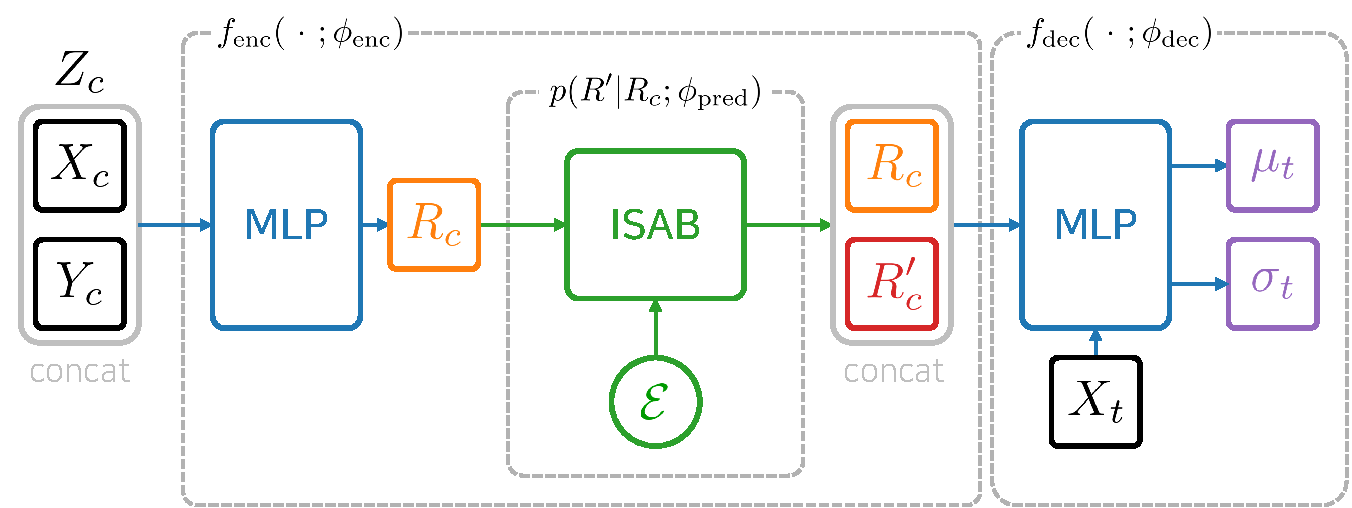
\includegraphics[width=\linewidth]{figure/main_concept.pdf}
    \caption{Concept figure of our feature generating model applied to \gls{cnp}~\citep{garnelo2018conditional}. We first convert given context dataset $Z_c$ to the representation $R_c$ using \gls{mlp} layers. Next we sample $\epsilon$ from a simple distribution (e.g. Gaussian). Then we generate the pseudo context representation $R_c'$ using generator as one layer \gls{isab}~\citep{lee2019set} in our experiment.
    %\ed{This figure is awesome!!}}
    }
    \label{figure/main_concept_mpnp}
\end{figure}
When $z$ is low-dimensional, it would be moderately easy to learn the joint predictives, but in practice, we often encounter problems with high-dimensional $z$, for instance when the input $x$ is a high-resolution image. For such cases, directly generating $z$ may be harder than the original problem, severely deteriorating the overall learning procedure of \gls{mpnp}.
Instead, we propose to generate the \emph{encoded representations} of $z$. The encoders of the most of the \glspl{npf} first encode an input $z_i$ into a representation $r_i$. For the remaining of the forward pass, we only need $r_i$s instead of the original input $z$. Hence we can build a joint predictives $p(R'|R_c; \phi_\text{pred})$ generating $R' = \{r_i'\}_{i=1}^{N-|c|}$ conditioned on $R_c = \{r_i\}_{i\in c}$ as for generating $Z'$ from $Z_c$. In the experiments, we compare these two versions of \glspl{mpnp} (generating $Z'$ and generating $R'$), and found that the one generating $R'$ works much better both in terms of data efficiency in training and predictive performances, even when the dimension of $z$ is not particularly large.
See \cref{figure/main_concept_mpnp} for our method applying to \gls{cnp} model~\citep{garnelo2018conditional}.

%%%%%%%%%%%%%%%%%%%%%%%%%%%%%%%%%%%%%%%%%%%%%%%%%%
\subsection{Training}\label{main:subsec:training}

With the generator $p(Z'|Z_c;\phi_\text{pred})$, the marginal likelihood for a task $\tau = (Z, c)$ is computed as
\[\label{eq:logmarginal_mp}
\log p(Y|X, Z_c) = \log\int \exp\bigg(-\sum_{i\in [n]}\ell(z_i, \tilde\theta(Z_c\cup Z'))\bigg) p(Z'|Z_c;\phi_\text{pred}) \dee Z'.
\]
Note that $p(Z'|Z_c;\phi_{\text{pred}})$ is \gls{cid}, so there exists a corresponding martingale posterior $\pi_N$ such that
\[
\log p(Y|X, Z_c) = \log\int \exp\bigg(-\sum_{i\in [n]}\ell(z_i, \theta)\bigg) \pi_N(\theta|Z_c) \dee \theta.
\]
We approximate the marginal likelihood via a consistent estimator,
\[\label{eq:mpnp_term1}
\log p(Y|X, Z_c) \approx \log \Bigg[ \frac{1}{K} \sum_{k=1}^K \exp\bigg(-\sum_{i\in [n]}\ell(z_i, \tilde\theta(Z_c\cup Z'^{(k)}))\bigg)
\Bigg] := -\calL_\text{marg}(\tau,\phi),
\]
where $Z'^{(1)},\dots, Z'^{(K)}\iidsim p(Z'|Z_c;\phi_\text{pred})$. This objective would be suffice if we are given sufficiently good $\tilde\theta(Z_c \cup Z'^{(k)})$, but we have to also train the encoder to properly amortize the parameter construction process \cref{eq:recovering_theta}. For this, we use only the given context data to optimize
\[\label{eq:mpnp_term2}
\log p_{\textsc{cnp}}(Y|X, Z_c) = -\sum_{i\in [n]} \ell(z_i, \tilde\theta(Z_c)) := -\calL_\text{amort}(\tau,\phi)
\]
that is, we train the parameters $(\phi_\text{enc}, \phi_\text{dec})$ using \gls{cnp} objective. Furthermore, we found that if we just maximize \cref{eq:mpnp_term1} and \cref{eq:mpnp_term2}, the model can cheat by ignoring the generated pseudo contexts and use only the original context to build function estimates. To prevent this, we further maximize the similar \gls{cnp} objectives for each generated pseudo context to encourage the model to actually make use of the generated contexts.
%\ljh{I'm not sure whether this justifies using avg outside the log rather than the avg inside the log.} 
\[\label{eq:mpnp_term3}
\frac{1}{K}\sum_{k=1}^K \log p_{\textsc{cnp}} (Y|X, Z'^{(k)}) = -\frac{1}{K}\sum_{i\in [n]} \ell(z_i, \tilde\theta(Z'^{(k)})) := -\calL_\text{pseudo}(\tau,\phi)
\]
Combining these, the loss function for the \gls{mpnp} is then
\[\label{eq:mpnp_term_whole}
\bbE_{\tau}[\calL(\tau,\phi)] = \bbE_\tau[\calL_\text{marg}(\tau,\phi) + \calL_\text{amort}(\tau,\phi) + \calL_\text{pseudo}(\tau,\phi)].
\]

% \lhg{I submitted our paper to Openreview. You can check that.}
% \ed{Thank you!!}

% \glspl{mpnp} model contains generator function $f_{\gen}$ which generates a pseudo context dataset $Z'$ or a feature of pseudo context dataset $R'$.
% To make a generator of \gls{mpnp} to sample meaningful $Z'$ or $R'$, we need to carefully construct training objective function. Otherwise, the generator tends to sample pseudo context dataset far from context dataset or collapse to one-point which does not have enough meaning or affection to target dataset. We maximize our training objective function which consists of the following terms:
% \begin{align}
%     \sum_{i=1}^n\left(\log p(y_i|x_i,Z_c,\varnothing)+\log \frac{1}{K}\sum_{k=1}^K p(y_i|x_i,Z_c,Z'^{(k)})+\frac{1}{K}\sum_{k=1}^K \log p(y_i|x_i, \varnothing, Z'^{(k)})\right)
% \end{align}
% % \ed{Thanks for updating, much clearer now. Should the third term be $p(y_i \mid x_i, \varnothing, Z'^{(k)})$ then?}
% % \lhg{Yes, that's right. We don't use context data in the third term.}\ed{I added it, hope it's ok!}
% where $K$ is the number of different generated pseudo context dataset.
% Here the first term $\log p(y|x,Z_c, \varnothing)$ implies that our amortized model should also well predict the posterior distribution of $Z$ only with context dataset. 
% The second term implies that the ensemble of our model should well predict the posterior distribution of $Z$ with context dataset and pseudo context dataset.
% The third term implies that our model should generate pseudo context dataset which well explains $Z$.
% This third term makes our model to actually generate more meaningful pseudo context dataset. 
% See \cref{app:sec:ablation_study} for generated pseudo context samples without third loss term.


% \ed{For the third term in (14), would it perhaps make more sense to put the sum inside the log, that is
% $$\log \frac{1}{K} \sum_{k=1}^K p(y_i \mid x_i, \varnothing, Z'^{(k)})$$
% so it is still kind of a posterior predictive density? Will this affect the results much?}\\
% \lhg{We empirical check that $\log \frac{1}{K} \sum_{k=1}^K p(y_i \mid x_i, \varnothing, Z'^{(k)})$ decrease the performances, and defeat by some baselines. And when I tried $\frac{1}{K} \sum_{k=1}^K \log p(y_i \mid x_i, \varnothing, Z'^{(k)})$, somewhat I think was each generated pseudo context set $Z'^{(k)}$ sampled independently and each sample should be sampled meaningfully. I mean if we use $\log \frac{1}{K} \sum_{k=1}^K p(y_i \mid x_i, \varnothing, Z'^{(k)})$, then the generator does not sample each pseudo context dataset meaningfully.}

% \lhg{
% \begin{align}
%     \log \Big(\frac{1}{K}\sum_{k=1}^K \exp{\big(\sum_{i=1}^n \log p(y_i|x_i,Z_c,Z'^{(k)})\big)}\Big) +\sum_{i=1}^n\left(\frac{1}{K}\sum_{k=1}^K \log p(y_i|x_i, \varnothing, Z'^{(k)}) + \log p(y_i|x_i,Z_c,\varnothing)\right)
% \end{align}
% }
% where $K$ is the number of different generated pseudo context dataset. Here, the first term is our posterior predictive density on $Z$, integrating over the posterior distribution of $\theta$ induced by the generator $p(Z_c' \mid Z_c)$.
% The second term  ensures our generator generates meaningful pseudo context dataset which allow the decoder to predict well.  As we are unable to evaluate the marginal likelihood $Z_c$ due to the implicit generative model, we rely on the decoder likelihood to improve the quality of $Z_c'$ samples. \lhg{For this term, we use $\frac{1}{K}\sum_{k=1}^K \log p(y_i|x_i, \varnothing, Z'^{(k)})$ instead of $\log\frac{1}{K}\sum_{k=1}^K  p(y_i|x_i, \varnothing, Z'^{(k)})$ to ensure that our generator samples each $Z'^{(k)}$s independently which well explains $Z$.} See \cref{app:sec:ablation_study} for generated pseudo context samples without this second loss term. The final term $\log p(y|x,Z_c, \varnothing)$ ensures that our amortized model also predicts well with only the context dataset. 

% \ed{Thanks for the explanation on log sum vs sum log - we should add a sentence to justify this. It looks a bit like the first term in the ELBO in equation (7). For the other point, I would prefer to leave in $\varnothing$, since the term $p(y_i \mid x_i,Z_c)$ is ambiguous, as it could be $p(y_i \mid x_i,Z_c, \varnothing)$ or $\int p(y_i \mid x_i,Z_c, Z_c') \, dp(Z_c' \mid Z_c)$. Please correct me if I'm wrong!}

% \lhg{Okay, that will be great. I added some explanations:) I have a Ph.D. admission interview next Tuesday at 16:30 KST so can we keep discussing by e-mail or comments? I understand that martingale posterior distribution is an open problem for model-data mismatch situations, is it correct?}

% \ed{Yes that's no problem, best of luck with the interview! :) @Juho should we cancel the Tuesday meeting then? We can communicate by email. Yep, model misspecification is still an open problem in the martingale posterior framework.}
% \lhg{Okay, great.}
% \ljh{No problem with me either!}

% \ed{The first term in the objective is more like the point-wise log posterior predictive density averaged over the $n$ data points, which is the KL divergence between the empirical distribution of $\mathcal{D}$ and the posterior predictive $p(y \mid x,Z_c)$.}

% \lhg{We changed our objective function. The first term changed from $\sum_{i=1}^n \log \frac{1}{K}\sum_{k=1}^K p(y_i|x_i,Z_c,Z'^{(k)})$ to $\log \Big(\frac{1}{K}\sum_{k=1}^K \exp{\big(\sum_{i=1}^n \log p(y_i|x_i,Z_c,Z'^{(k)})\big)}\Big)$.}

% \ed{
% % Nice!! And this work well? The objective is looking much better motivated now :) 
% % For the third term, we previously tried putting the avg inside the log, that is
% % $$\sum_{i \in [n]} \log \frac{1}{K} \sum_{k =1}^K  \exp\left(-\ell(z_i, \tilde\theta(Z'^{(k)}))\right),$$ and it didn't work well right? 
% Following the recent change to $\mathcal{L}_{\text{marg}}$, what about 
% $$
%  -\mathcal{L}_{\text{pseudo}}^*(\phi) =  \log \frac{1}{K} \sum_{k =1}^K  \exp\left(-\sum_{i \in [n]} \ell(z_i, \tilde\theta(Z'^{(k)}))\right),
% $$
% which is basically the first term, so a marginal likelihood, but only using $Z'^{(k)}$. The current $-\mathcal{L}_{\text{pseudo}}$ is a just lower bound on $-\mathcal{L}_{\text{pseudo}}^*$ from Jensen's inequality. 
% %Because of this, I'm guessing the results will be similar. 
% The objective would be nice and symmetric now, since it's essentially 3 (marginal) likelihood terms, corresponding to context + pseudo, only context and only pseudo.
% % If we're short on time, we can motivate $-\mathcal{L}_{\text{pseudo}}$ as being a lower bound to $-\mathcal{L}^*_{\text{pseudo}}$, that is perhaps numerically more stable. Really sorry for giving you more work Hyungi!!
% }
% \lhg{Actually, we simultaneously tried that term in experiment with (18) and sadly it didn't work well...So we fixed (18). Maybe we can justify with lower bound or something else.}
% \ed{Ah damn, that's unfortunate. Maybe we can stick to the lower bound justification then and point to the Supplementary.}
% \lhg{Yep, that will be good. Now we are trying $\lambda\calL^*$ with additional scaling factor $\lambda\geq 1$.}
% \ed{That's a good idea, perhaps we need to balance $\mathcal{L}_{\text{pseudo}}$ with $\mathcal{L}_{\text{amort}}$?}
% \lhg{That's a good point.}
% \paragraph{Main approach}
% \glspl{np} are interested in learning a latent function $f$ such that
% \begin{align*}
%     f\sim p(f),\quad y|x,f\sim p(y|x,f)
% \end{align*}
% where $(x,y)\in \calD$.
% For instance, $f$ may be parameterized by decoder neural networks of \glspl{np}, $\mu_{\dec}(\cdot;\theta)$ and $\sigma_{\dec}(\cdot;\theta)$, such that
% \begin{align*}
%     \theta\sim p(\theta),\quad y|x,\theta\sim \calN(y|\mu_{\dec}(x;\theta),\sigma_\dec^2 (x;\theta)).
% \end{align*}
% In martingale posterior neural processes, instead of assuming a prior (either for $p(f)$ or $p(\theta)$), we directly model a conditional joint predictive distributions of pseudo context dataset as,
% \begin{align*}
%     \calD_{C'}\sim p_\phi (\calD_{C'}|\calD_C),
% \end{align*}
% where $\phi$ is a parameter of joint predictive distribution and $\calD_{C'}=\{(x_i',y_i')\}_{i=1}^{n_g}$ is a generated pseudo context dataset with number of generated pseudo context data $n_g\geq 1$.
% If $(x,y)$ is high-dimensional (such as images), we can instead consider an encoded vector $r_C=f_{\enc}(\calD_C)$ and learn the joint predictive distribution of the encoded representations as $p_\phi (r_{C'}|r_C)$. Using this predictive, we can construct an empirical predictive density as
% \begin{align*}
%     g_N(x,y) = \frac{1}{|c|+n_g}\left(\sum_{i\in c}\delta_{(x_i,y_i)} + \sum_{i=1}^{n_g}\delta_{(x_i',y_i')}\right).
% \end{align*}
% The estimate of the function parameter $\theta$ should originally be obtained as
% \begin{align*}
%     \theta(g_N):=\argmin_\theta\int \ell((x,y),\theta)g_N(dx,dy),
% \end{align*}
% where in our case we set
% \begin{align*}
%     \ell((x,y),\theta)=-\log \calN (y|\mu_{\dec}(x;\theta),\sigma_{\dec}^2(x;\theta)).
% \end{align*}
% Instead of directly solving this, we introduce an amortization network with parameter $\lambda$ such that
% \begin{align*}
%     \hat{\theta}(\calD_C\cup\calD_{C'};\lambda)\approx \theta(g_N).
% \end{align*}
% Here we can see that differently generated pseudo context dataset $\calD_{C'}^{(1)}=\{(x_i'^{(1)},y_i'^{(1)})\}_{i=1}^{n_g}$ and $\calD_{C'}^{(2)}=\{(x_i'^{(2)},y_i'^{(2)})\}_{i=1}^{n_g}$ formulate different empirical predictive densities.
% Different predictive densities also formulate different amortized $\hat{\theta}$ which models functional uncertainty without both a global latent variable and a custom prior distribution.
% If we have chosen to learn the predictive of encoded representations, we first have to learn $\hat{\theta}(\cdot;\lambda)$ using only real context representation $r_C$, and put generated representation $r_{C'}$ into the amortization network later.
% \paragraph{Directly generating pseudo context data}
% In order to construct an empirical predictive density $g_N(x,y)$, we have to sample a pseudo context dataset. 
% The most straightforward approach to generate pseudo context dataset $\calD_{C'}$ is directly generating $(x_i',y_i')$ from given context dataset $\calD_C$.
% Our first attempt to formulate generator function $f_{\gen}$ was to na\"ively use ISAB~\citep{lee2019set} module as our generator and sample whole $D_{C'}$ at once.
% We use concatenated $D_C$ as inducing points $I\in\bbR^{|C|\times 2}$ in ISAB and $g$, which is \textit{i.i.d} samples from Gaussian distribution, as input $\bx\in \bbR^{n_g\times 2}$.
% Because ISAB module satisfies permutation invariance for input dataset, we can directly sample a set $\calD_{C'}$ without break exchangeability...
% \paragraph{Generating features of pseudo context data}
% \begin{figure}[t]
%     \centering
%     \includegraphics[width = \linewidth]{figure/feature model2.pdf}
%     \caption{Concept figure of our feature generating model applied to \gls{canp}~\citep{kim2018attentive}. Here we sample $g$ from a simple distribution (e.g. Gaussian). We generate key feature $r_k'$ and value feature $r_v'$ for cross attention layer which are corresponding to pseudo context data. We use generator as one layer ISAB~\citep{lee2019set} in our experiment.}
%     \label{fig:feature model2.pdf}
% \end{figure}
% As we mentioned above paragraph, directly generating pseudo context dataset is hard task, we construct our model to sample features of pseudo context dataset.
% We first encode our $\calD_c$ into $r_c\in\bbR^{|C|\times r_\text{dim}}$ with our encoder neural network $f_{\enc}$.

% See \cref{fig:feature model2.pdf} for our method applying to \gls{canp} model~\citep{kim2018attentive}.
% \subsection{Training}
% \label{main:subsec:training}
% \glspl{mpnp} model contains generator function $f_{\gen}$ which generates a pseudo context dataset $\calD_{C'}$ or a feature of pseudo context dataset $r_{C'}$.
% To make a generator of \gls{mpnp} to sample meaningful $\calD_{C'}$ or $r_{C'}$, we need to carefully construct training objective function. Otherwise, the generator tends to sample pseudo context dataset far from context dataset or collapse to one-point which does not have enough meaning or affection to target dataset. We consist our training objective function as maximizing following terms:
% \begin{align}
%     \sum_{i=1}^n\left(\log p(y_i|x_i,\calD_C)+\log \frac{1}{K}\sum_{j=1}^K p(y_i|x_i,\calD_C,\calD_{C'}^{(j)})+\frac{1}{K}\sum_{j=1}^K \log p(y_i|x_i, \calD_{C'}^{(j)})\right)
% \end{align}
% \ed{Does the $p$ in the first term above need a subscript? So something like $p_{\text{amort}}$ or something?}

% where $K$ is the number of different generated pseudo context dataset.
% Here the first term $\log p(y|x,\calD_C)$ implies that our amortized model should also well predict the posterior distribution of $\calD$ only with context dataset. 
% The second term implies that the ensemble of our model should well predict the posterior distribution of $\calD$ with context dataset and pseudo context dataset.
% The third term implies that our model should generate pseudo context dataset which well explains $\calD$.
% This third term makes our model to actually generate more meaningful pseudo context dataset. 
% See \cref{app:sec:ablation_study} for generated pseudo context samples with and without each loss terms.

%%%%%%%%%%%%%%%%%%%%%%%%%%%%%%%%%%%%%%%%%%%%%%%%%%
\section{Related Works}
\label{main:sec:related}
%%%%%%%%%%%%%%%%%%%%%%%%%%%%%%%%%%%%%%%%%%%%%%%%%%
\gls{cnp}~\citep{garnelo2018conditional} is the first \gls{npf} model which consists of simple \gls{mlp} layers as its encoder and decoder. \gls{np}~\citep{garnelo2018neural} also uses \gls{mlp} layers as its encoder and decoder but introduces a global latent variable to model a functional uncertainty.
\gls{canp}~\citep{kim2018attentive} and \gls{anp}~\citep{kim2018attentive} are the models which apply attention modules as their encoder block in order to well summarize context information relevant to target points. 
\citet{louizos2019functional} proposed \glspl{np} model which employs local latent variables instead of a global latent variable by applying a graph neural network.
By applying convolution layers as their encoder, \citet{gordon2020convolutional} and \citet{foong2020meta} introduced a translation equivariant \glspl{cnp} and \glspl{np} model, respectively. 
In addition to these works, \gls{bnp}~\citep{lee2020bootstrapping} suggests modeling functional uncertainty with the bootstrap~\citep{efron1992bootstrap} method instead of using a single global latent variable. 
% \gls{neubnp}~\citep{lee2022neural} also used a recent bootstrap method called Neural Bootstrapper~\citep{shin2021neural} to model functional uncertainty.

\section{Experiments}

\subsection{Communication Efficiency at Scale}\label{sect:experiments_square_cube}

Before we can meaningfully evaluate SWARM parallelism, we must verify our theoretical observations on communication efficiency. Here we run several controlled experiments that measure the GPU utilization and network usage for different model sizes, using the Transformer architecture~\citep{transformer} that has been widely adopted in various fields~\citep{lin2021survey}. To decouple the performance impact from other factors, we run these experiments on homogeneous V100 GPU nodes that serve one pipeline stage over the network with varying latency and bandwidth. We use a batch size of 1 and sequences of 512 tokens; the complete configuration is deferred to Appendix~\ref{appendix:detailed_setup}.


First, we measure how the model size affects the computation to communication ratio at 500 Mb/s network bandwidth in both directions. We consider 4 model configurations: the base configuration from the BERT paper~\citep{bert}, ``xxlarge" (``large'' with $d_{model}{=}4096$),  which is used in several recent works~\citep{albert,ernie3,deberta}, and a GPT-3-scale model with $d_{model}{=}12288$~\citep{gpt3}. We also evaluate a modified Transformer architecture (``Ours'') as defined in Section~\ref{sect:experiments_large} with $d_{model}{=}4096$, 3 layers per pipeline stage and 8-bit quantized activations. As we demonstrate in Appendix~\ref{appendix:compression}, this compression strategy can significantly reduce network usage with little effect on convergence. In the first three configurations, the model consists of 12 Transformer layers placed on 12 servers with a single GPU; in the last one, there are 4 servers, each hosting 3 layers.
Appendix~\ref{appendix:detailed_setup} contains FLOP and parameter counts of each configuration.




\begin{figure}[b]
\vspace{-14pt}
    \centering
    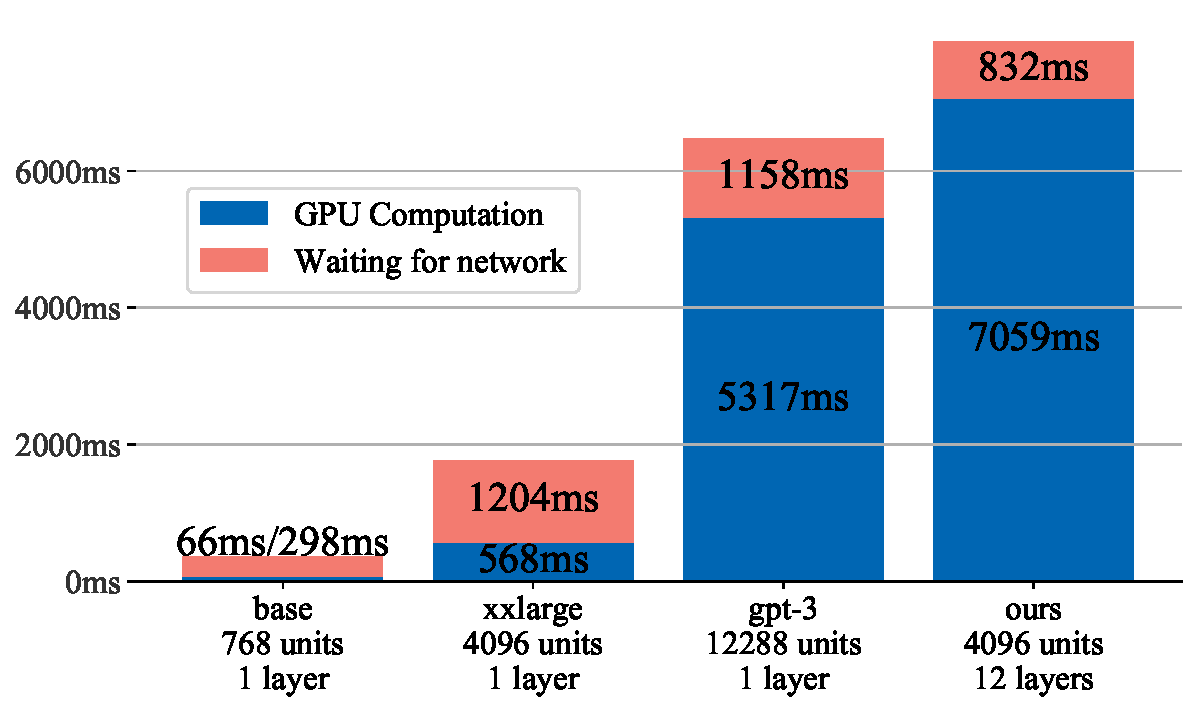
\includegraphics[width=1\linewidth]{resources/perf_absolute.pdf}
    \vspace{-12pt}
    \captionof{figure}{Pipeline computation and idle time per batch at 500 Mb/s bandwidth.}
    \label{fig:throughput_exps}
\end{figure}%
\begin{table}
    \centering
    \captionof{table}{Relative device utilization at 500 Mb/s bandwidth and varying network latency.}
    \label{tab:latency}
    \small
    \setlength{\tabcolsep}{8pt}
    \begin{tabular}[b]{@{}lcccc@{}}
    \toprule
    \multirow{2}{*}{\thead{Latency\\(RTT)}} & 
    \multicolumn{4}{c}{
    \thead{
    Relative GPU utilization\\ (100\% - idle time)
    }
    }
    
    \\
\cmidrule{2-5}                     & base & xxlarge & GPT-3 & Ours \\ \midrule
    None &   18.0\%     &  32.1\%         &  82.1\%  &  89.5\%      \\
    10ms &   11.8\%      &   28.9\%    &   79.3\%   &  87.2\%    \\
    50ms &    4.88\%      &   20.1\%    &   70.3\% &  79.5\%    \\
    100ms &    2.78\%      &    14.9\%    &  60.2\%     &   71.5\% \\
    200ms &   1.53\%     &  10.1\%    &  48.5\%   &     59.2\%    \\
    \bottomrule
    \end{tabular}
    \vspace{-6pt}
\end{table}

As depicted in Figure~\ref{fig:squarecube} (right) and Figure~\ref{fig:throughput_exps}, larger models achieve better GPU utilization rate in the same network conditions, since their communication load grows slower than computation. More importantly, even at 500 Mb/s, the resulting GPU idle time can be pushed into the 10--20\% range, either naturally for GPT-3-sized models or through activation compression for smaller models. In addition, large models maintain most of their training efficiency at the 100ms latency~(Table~\ref{tab:latency}), which is roughly equivalent to training on different continents~\citep{verizon_latency}.

\vspace{-4pt}
\subsection{Detailed Performance Comparison}\label{appendix:training_throughput}

Here we investigate how SWARM parallelism compares to existing systems for training large models: \textbf{GPipe}~\citep{huang2019gpipe} and \textbf{ZeRO-Offload}~\citep{zerooffload}.
The purpose of this section is to compare the training throughput in ``ideal'' conditions (with homogeneous reliable devices and balanced layers), as deviating from these conditions makes it \textit{infeasible} to train with baseline systems.
Still, even in such conditions the performance of different systems can vary across model architectures, and hence we want to identify the cases in which using SWARM is preferable to other approaches.
We benchmark individual SWARM components in preemptible setups in Section~\ref{sect:experiments_adaptive} and Appendix~\ref{appendix:scaling}.

We evaluate training performance for sequences of 4 Transformer layers of identical size distributed over 16 workers. Similarly to Section~\ref{sect:experiments_square_cube}, we use three layer configurations: ``xxlarge''~($d_{model} {=} 4096$, $d_{\text{FFN}} {=} 16384$, 32 heads), ``GPT-3''~($d_{model} {=} 12288$, $d_{\text{FFN}} {=} 49152$, 96 heads), and ``Ours''~($d_{model} {=} 4096$, $d_{\text{FFN}} {=} 16384$, 32 heads, 16 shared layers per block, last stage holds only the vocabulary projection layer). The microbatch size is 4 for ``xxlarge'' and 1 for ``GPT-3'' and ``Ours'', and the sequence length is 512.

To provide a more detailed view of the training performance, we measure two separate performance statistics: the training throughput and the All-Reduce time. 
The training throughput measures the rate at which the system can process training sequences, i.e., run forward and backward passes. 
More specifically, we measure the time required to process 6250 sequences of 512 tokens, which corresponds to the largest batch size used in~\citet{gpt3}.
In turn, the All-Reduce time is the time each system spends to aggregate accumulated gradients across devices. 
Intuitively, training with small batch sizes is more sensitive to the All-Reduce time (since the algorithm needs to run All-Reduce more frequently) and vice versa.


\textbf{Hardware setup:} Each worker uses a V100-PCIe GPU with 16 CPU threads (E5 v5-2660v4) and 128 GB RAM. The only exception is for ZeRO-Offload with ``GPT-3'' layers, where we had to double the RAM size because the system required 190 gigabytes at peak. Similarly to Section~\ref{sect:experiments_square_cube}, each worker can communicate at a 500 Mb/s bandwidth for both upload and download for a total of 1 Gb/s.
In terms of network latency, we consider two setups: with \textbf{no latency}, where workers communicate normally within the same rack, and with \textbf{latency}, where we introduce additional $100\pm50$ms latency directly in the kernel\footnote{More specifically, \texttt{tc qdisc add dev <...> root netem delay 100ms 50ms}}.

\textbf{GPipe configuration:} We use a popular PyTorch-based implementation of GPipe\footnote{The source code is available at \url{https://github.com/kakaobrain/torchgpipe}}. The model is partitioned into 4 stages repeated over 4 model-parallel groups. To fit into the GPU memory for the ``GPT-3'' configuration, we offload the optimizer into RAM using ZeRO-Offload. Before averaging, we use PyTorch's built-in All-Reduce to aggregate gradients.
We evaluate both the standard GPipe schedule and the 1F1B schedule~\citep{pipedream}.

\textbf{ZeRO-Offload configuration:} Each worker runs the entire model individually, then exchanges gradients with peers. For ``xxlarge'', we use the official implementation from~\cite{zerooffload}. However, for ``GPT-3'', we found that optimizer offloading still does not allow us to fit 4 layers into the GPU. For this reason, we also offload the model parameters using the \texttt{offload\_param} option.

\begin{table}
\centering
\small
\setlength{\tabcolsep}{4pt}
\captionof{table}{Training performance for different model sizes.}
\label{tab:throughput_gpt}
\begin{tabular}[b]{lcccc}
\toprule
\multirow{2}[2]{*}{System} &
  \multicolumn{2}{c}{Throughput, min/batch} &
  \multicolumn{2}{c}{All-Reduce time, min} \\ \cmidrule(lr){2-3}\cmidrule(lr){4-5} 
                 & No latency & Latency & No latency & Latency \\
 \midrule \multicolumn{5}{c}{``GPT-3'' (4 layers) }\\
 \midrule
SWARM            &  168.3 &\textbf{186.7}  &  7.4 & \textbf{7.6}   \\
GPipe            &  164.5 & 218.4 &  \multirow{2}{*}{\textbf{6.7}}    & \multirow{2}{*}{7.8}   \\
1F1B & \textbf{163.3} & 216.1 & & \\
Offload          &  272.7 & 272.7          &  25.5 & 27.3 \\
\midrule \multicolumn{5}{c}{``xxlarge'' (4 layers) }\\
\midrule
SWARM            &  44.2 & 48.2                  &  0.8  & \textbf{0.9}   \\
GPipe            &  40.1 & 108.8                  &  \multirow{2}{*}{\textbf{0.7}}  & \multirow{2}{*}{1.1}   \\
1F1B & 40.8 & 105.5 & & \\
Offload          &  \textbf{33.8} & \textbf{33.8}  &  2.8 & 4.2   \\
\midrule \multicolumn{5}{c}{Full ``Ours'' model (48 shared layers + embeddings) }\\
\midrule
SWARM            &  432.2 & 452.9                  &  0.8  &\bf 1.0   \\
GPipe            &  420.0 & 602.1                   &  \multirow{2}{*}{\bf 0.7}  & \multirow{2}{*}{1.1}   \\
1F1B             &  408.5 & 569.2 & & \\
Offload          &  \bf 372.0 &\bf 372.0  &  3.2 & 4.8   \\
\bottomrule
\end{tabular}
\vspace{-8pt}
\end{table}%

\begin{figure}[b]
\vspace{-16pt}
\centering
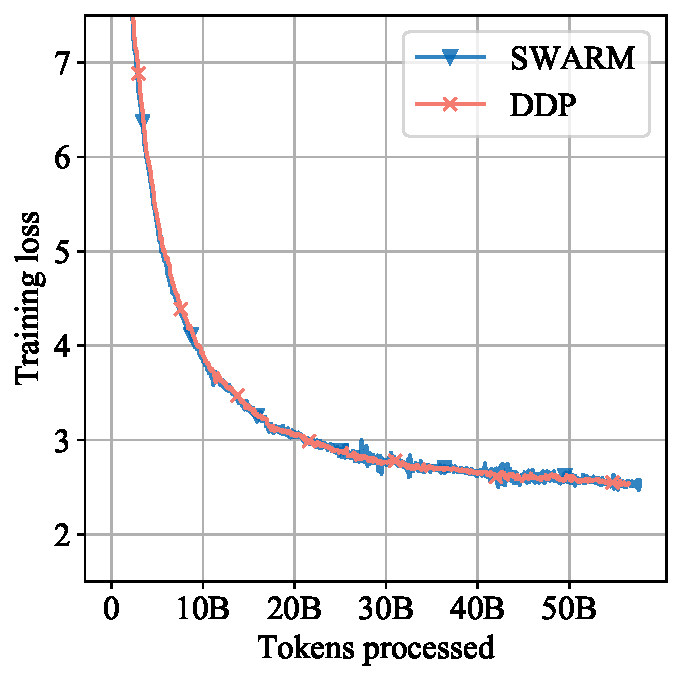
\includegraphics[ width=0.65\linewidth]{resources/learning_3stages.pdf}
\vspace{-6pt}
\captionof{figure}{Training convergence comparison.}
\label{fig:convergence}
\end{figure}

In turn, when training smaller models, ZeRO-Offload outperforms both SWARM and GPipe. This result aligns with our earlier observations in Figure~\ref{fig:squarecube}, where the same model spent most of the time waiting for the communication between pipeline stages.%

We also observe that ZeRO-Offload takes longer to aggregate gradients, likely because each peer must aggregate the entire model, whereas in SWARM and GPipe, peers aggregate a single pipeline stage. The variation between All-Reduce time in GPipe and SWARM is due to implementation differences. Overall, SWARM is competitive to HPC baselines even in an idealized homogeneous environment.

\subsection{Large-Scale Distributed Training}
\label{sect:experiments_large}

To verify the efficiency of SWARM parallelism in a practical scenario, we conduct a series of large-scale distributed experiments using preemptible (unreliable) cloud T4 and A100 GPUs over a public cloud network.

We train a Transformer language model with the architecture similar to prior work~\citep{gpt3,gptj,gptneo} and 1.01 billion parameters in total. Our model consists of 3 stages, each containing a single Transformer decoder block with $d_{model}=4096$ and 16 layers per pipeline stage. All workers within a stage serve the same group of layers, and all layers within each group use the same set of parameters, similarly to ALBERT~\citep{albert}. On top of this, the first stage also contains the embedding layer, and the last stage includes the language modeling head. Because of layer sharing, this model is equivalent to a 13B model from~\citet{gpt3} in terms of compute costs. 

We use 8-bit compression~\citep{adam8bit} for activations and gradients to reduce the communication intensity. Additional training setup details are covered in Appendix~\ref{appendix:detailed_large}.
SWARM nodes run rebalancing every $T=300$ seconds, and trainers measure peer performance using a moving average with $\alpha=0.1$. However, as we show in Section~\ref{sect:experiments_adaptive}, the throughput of SWARM is not very sensitive to the choice of these hyperparameters.



First, to verify that model parallelism with asynchronous updates does not have significant convergence issues, we train the model on the Pile~\citep{gao2020pile} dataset with 400 preemptible T4 instances, each hosting one accelerator. As a baseline, we use regular data-parallel training with offloading on 128 A100 GPUs.
We run both experiments for approximately 4 weeks and compare the learning curves.




Figure~\ref{fig:convergence} shows the results of this experiment: it can be seen that the training dynamics of two approaches are indeed similar, which demonstrates the viability of SWARM parallelism for heterogeneous and poorly-connected devices.

In the next experiment, we aim to measure the pipeline throughput in different hardware conditions and to compare it with an estimate of best-case pipeline performance.
We consider several setups: first, we use the same 400 preemptible T4 nodes; in another setup, we use 7 instances with 8 A100 GPU each; finally, we combine these fleets to create a heterogeneous setup. We examine the performance of the pipeline both with weight sharing and with standard, more common, Transformer blocks.

\begin{table}
\centering
\captionof{table}{Pipeline throughput, layer sharing.}
\label{tab:throughput}
\small
\begin{tabular}{@{}lcccc@{}}
\toprule
\multirow{2}{*}{\begin{tabular}[c]{@{}l@{}}Hardware\\ setup\end{tabular}} &
  \multicolumn{2}{c}{\begin{tabular}[c]{@{}c@{}}Throughput,\\ samples/s\end{tabular}} &
  \multicolumn{2}{c}{\begin{tabular}[c]{@{}c@{}}Optimal\\ bandwidth, Mb/s\end{tabular}} \\ \cmidrule(lr){2-3}\cmidrule(lr){4-5} 
                 & Actual & Best-case & Upload & Download \\ \midrule
T4           &  17.6      &   19.2        &   317.8     &     397.9     \\
A100          & 16.9       &   25.5        &   436.1     &     545.1     \\
T4 \& A100 &   27.3     &       ---    &   ---     &      ---    \\ \bottomrule
\end{tabular}
\end{table}
\begin{table}
\centering
\captionof{table}{Pipeline throughput, default Transformer.}
\label{tab:throughput_standard}
\small
\begin{tabular}{@{}lcc@{}}
\toprule
\multirow{2}{*}{\begin{tabular}[c]{@{}l@{}}Hardware\\ setup\end{tabular}} &
  \multicolumn{2}{c}{\begin{tabular}[c]{@{}c@{}}Throughput,\\ samples/s\end{tabular}} \\ \cmidrule(lr){2-3}
                 & Actual & Best-case \\ \midrule
T4           &  8.8      &   19.3        \\
A100          & 8.0       &   25.1        \\
T4 \& A100 &   13.4     &       ---    \\ \bottomrule
\end{tabular}
\end{table}






We measure the number of randomly generated samples processed by the pipeline both in our infrastructure and the ideal case that ignores all network-related operations (i.e., has infinite bandwidth and zero latency). The ideal case is emulated by executing a single pipeline stage 3 times locally on a single server and multiplying the single-node estimates by the number of nodes.

As demonstrated in the left two columns of Table~\ref{tab:throughput} and Table~\ref{tab:throughput_standard}, asynchronous training of compute-intensive models with 8-bit compressed activations regardless of the architecture specifics allows us to achieve high performance without a dedicated networking solution. Furthermore, the load balancing algorithm of SWARM allows us to dynamically and efficiently utilize different hardware without being bottlenecked by slower devices. 


Next, we use the same load testing scenario to estimate the bandwidth required to fully utilize each device type in the above infrastructure. For this, we measure the average incoming and outgoing bandwidth on the nodes that serve the intermediate stage of the pipeline. We summarize our findings in the right two columns of Table~\ref{tab:throughput}: it turns out that with layer sharing and 8-bit compression, medium-performance GPUs (such as T4) can be saturated even with moderate network speeds. Based on our main experiment, the optimal total bandwidth is roughly 100Mb/s higher than the values reported in Table 3 due to gradient averaging, loading state from peers, maintaining the DHT and streaming the training data.
Although training over the Internet with more efficient hardware might indeed underutilize the accelerator, this issue can be offset by advanced compression strategies such as compression-aware architectures or layer sharing, as shown in Table~\ref{tab:throughput}.

\begin{figure}[t]
    \centering
    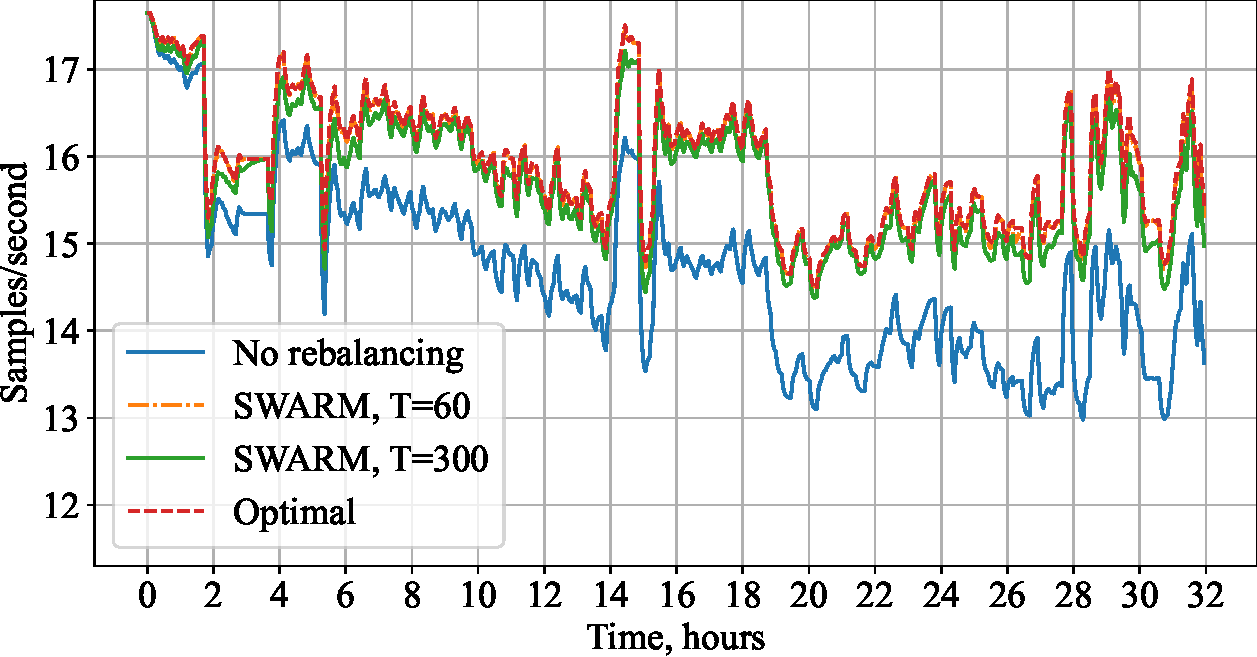
\includegraphics[width=\linewidth]{resources/rebalancing_activity.pdf}
    \captionof{figure}{Throughput of rebalancing methods over time.}
    \label{fig:rebalancing}
\end{figure}

\subsection{Adaptive Rebalancing Evaluation}


\begin{figure*}[h!]
\begin{subfigure}{0.5\textwidth}
    \centering
    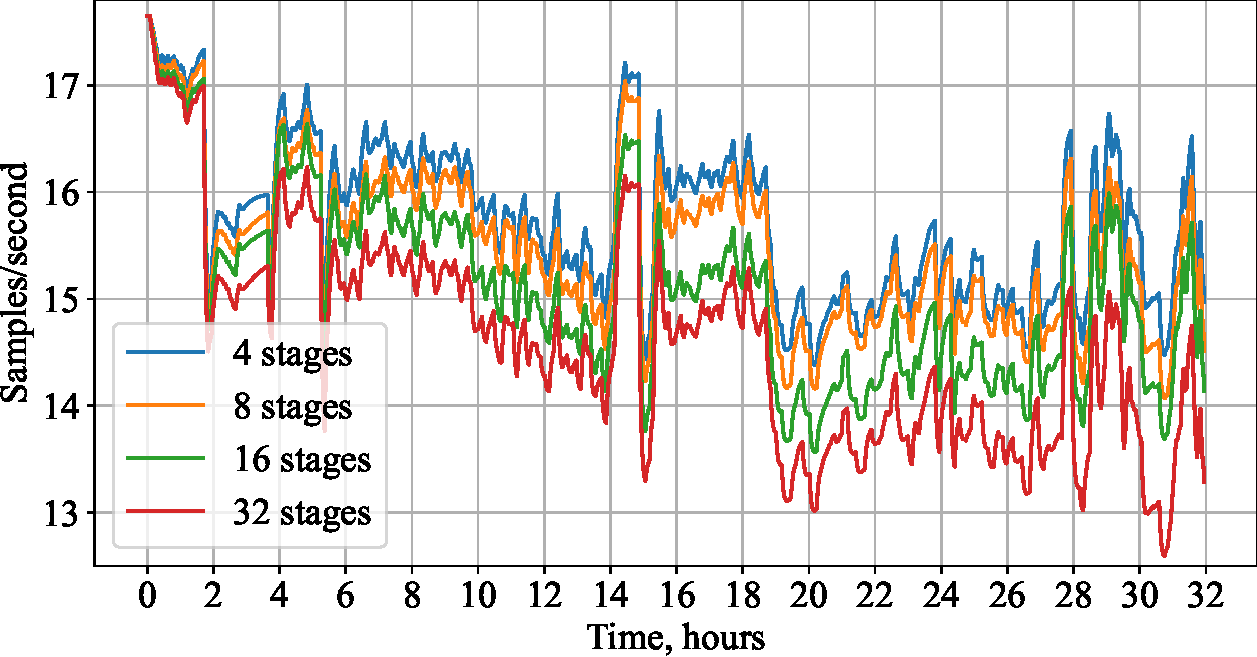
\includegraphics[width=0.97\linewidth]{resources/rebalancing_stages.pdf}
    \caption{Adaptive rebalancing of SWARM parallelism.}
    \label{fig:rebalancing_stages}
\end{subfigure}%
\begin{subfigure}{0.5\textwidth}
    \centering
    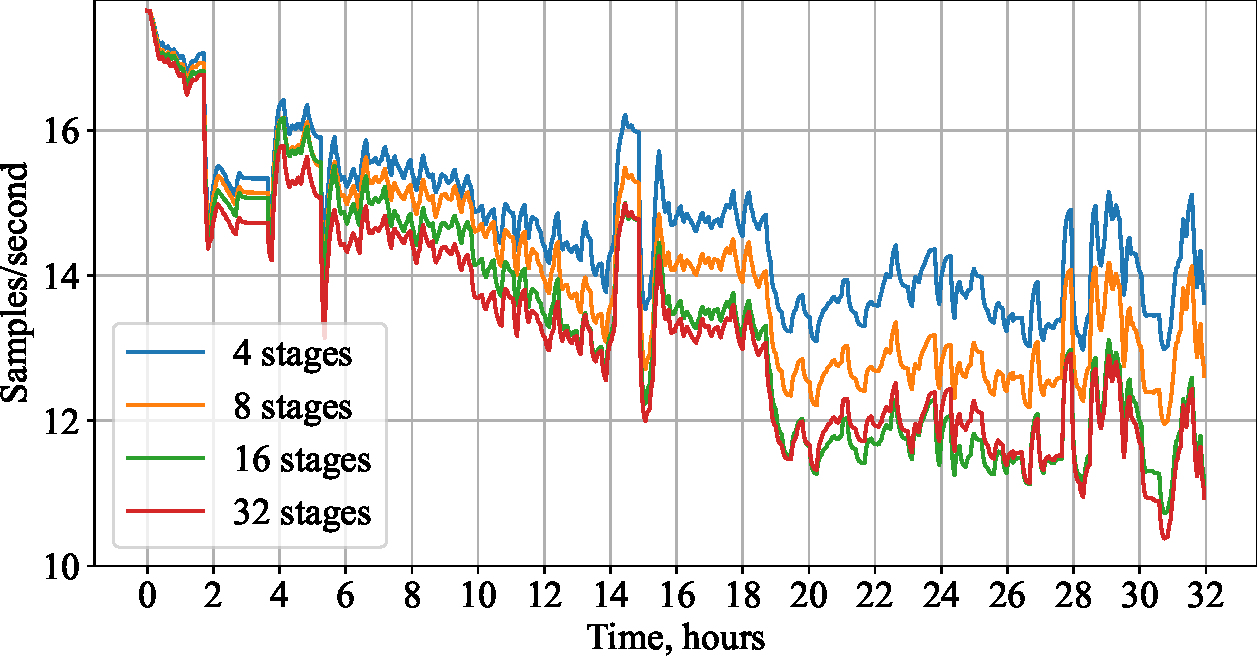
\includegraphics[width=0.97\linewidth]{resources/rebalancing_stages_baseline.pdf}
    \caption{No rebalancing.}
    \label{fig:rebalancing_stages_baseline}
\end{subfigure}
\caption{Scaling of pipeline-parallel strategies with respect to the number of stages.}
\label{fig:rebalancing_stages_all}
\end{figure*}

\label{sect:experiments_adaptive}
In this experiment, we evaluate the efficiency of adaptive peer rebalancing between stages proposed in Section~\ref{sect:method_swarm}. 
We use statistics of the number of active T4 nodes from the 32-hour segment of the experiment described in Section~\ref{sect:experiments_large}. 
We use this data to simulate training dynamics by viewing it as sequence of events, each consisting of a timestamp and a change in the number of peers (which can be positive or negative). 
When a worker is removed from the pipeline, we randomly choose the stage it was removed from: that is, removing $N$ peers corresponds to $N$ samples from the uniform distribution over four pipeline stages. 
We run 10 simulations with different random seeds and average the resulting trajectories.
We compare our strategy with two different values of $T$ to the baseline that has no rebalancing.

The results of this evaluation are available in \autoref{fig:rebalancing}; for reference, we also provide the performance of a theoretically optimal rebalancing strategy that maintains the highest possible throughput at every moment. It can be seen that even with the rebalancing period $T=300$, our approach significantly improves the overall throughput of the pipeline. When the number of peers is relatively stable, the rebalanced pipeline also approaches the optimal one in terms of throughput, which shows the efficiency of rebalancing even when moving only one node at a time.

In addition, we observed that for some brief periods, the performance of the unbalanced pipeline exceeded the throughput of the balanced one due to random choice of disconnecting peers (dropping more from the ``overrepresented'' stages affects the imbalanced pipeline less). However, this held true only for $\approx 4.5\%$ of the experiment and was quickly mitigated by adaptive rebalancing.

As expected, decreasing $T$ from 300 to 60 seconds improves both the overall throughput and the speed of convergence to optimal pipeline performance. However, the effect is not as drastic compared to the increase in DHT data transfer volume. This is also demonstrated by \autoref{tab:rebalancing_speedup}, which shows the relative throughput of the three configurations compared to the optimal one. Furthermore, the table displays that while initially there is little difference between rebalancing choices, it becomes more pronounced later on as the imbalanced version ``drifts further'' from the optimal state.

\begin{table}[b]
\centering
\captionof{table}{Relative throughput comparison of pipeline rebalancing methods.}
\small
\label{tab:rebalancing_speedup}
\begin{tabular}[b]{@{}lccc@{}}
\toprule
\multirow{2}[2]{*}{\thead{Rebalancing}} & \multicolumn{3}{c}{\% of optimal} \\ \cmidrule(l){2-4} 
                        & Overall   & First 1 hour   & Last 1 hour  \\ \midrule
None                & 82.7      & 99.0       & 45.4     \\
$T=300$    & 95.8      & 99.4       & 88.9     \\
$T=60$     & 97.6      & 99.8       & 91.7     \\ \bottomrule
\end{tabular}
\end{table}

Finally, we analyze the scaling properties of rebalancing with respect to the number of stages. To do this, we conduct experiments in the same setup as above ($T=300$) while changing the number of pipeline stages from 4 to $\{4,\ 8,\ 16,\ 32\}$. To ensure the consistency of throughput across all experiments, we increase the starting number of peers accordingly while keeping the preemption rate constant. As a baseline, we also evaluate the throughput of the pipeline that has no rebalancing.

Figure~\ref{fig:rebalancing_stages_all} shows the outcome of this experiment. As displayed in the plots, both strategies drop in performance with the increase in the stage count: while all stages should drop in performance equally in expectation, in practice, the variances are too large while the number of peers is relatively too small for the asymptotic properties to take place. This effect results in more outliers (large drops in the number of peers) in the preemption distribution for more stages. Still, rebalancing allows to partially mitigate the issue: while we observe a more consistent downward trend for the baseline strategy, the rebalanced pipeline regains its performance over time and achieves a higher overall throughput.


\section{Conclusion}
In this work, we advance the method of {machine unlearning} through a novel viewpoint: model sparsification, achieved by weight pruning. We show in both theory and practice that model sparsity plays a foundational and crucial role in closing the gap between exact unlearning and existing approximate unlearning methods. Inspired by that, we propose two new unlearning paradigms,  `prune first, then unlearn' and `sparsity-aware unlearn', which can significantly improve the efficacy of approximate unlearning. We demonstrate the effectiveness of our findings and proposals in extensive experiments across different unlearning setups. Our study also indicates the presence of \textit{model modularity} traits, such as weight sparsity, that could simplify the process of machine unlearning. This may open up exciting prospects for future research to investigate unlearning patterns within weight or architecture space.





\clearpage
\newpage
\paragraph{Societal Impacts}
Our work is unlikely to bring any negative societal impacts. Modeling functional uncertainty may be related to the discussion of safe AI within the community.

\paragraph{Reproducibility Statement}
We argued our experimental details in \cref{app:sec:details} which contains used libraries and hardwares.
We presented all the dataset description in \cref{app:sec:details}.
We describes the model architecture details in \cref{app:sec:architectures}.

\section*{Acknowledgements}
This work was partly supported by Institute of Information \& communications Technology Planning \& Evaluation (IITP) grant funded by the Korea government(MSIT) 
(No.2019-0-00075, Artificial Intelligence Graduate School Program(KAIST)), Institute of Information \& communications Technology Planning \& Evaluation (IITP) grant funded by the Korea government(MSIT) (No.2022-0-00713), and Institute of Information \& communications Technology Planning \& Evaluation (IITP) grant funded by the Korea government(MSIT) (No.2021-0-02068, Artificial Intelligence Innovation Hub).
\bibliography{references}

\clearpage
\newpage
\appendix

%%%%%%%%%%%%%%%%%%%%%%%%%%%%%%%%%%%%%%%%%%%%%%%%%%
\section{Model Architectures}
\label{app:sec:architectures}
%%%%%%%%%%%%%%%%%%%%%%%%%%%%%%%%%%%%%%%%%%%%%%%%%%

\begin{figure}[t]
    \centering
    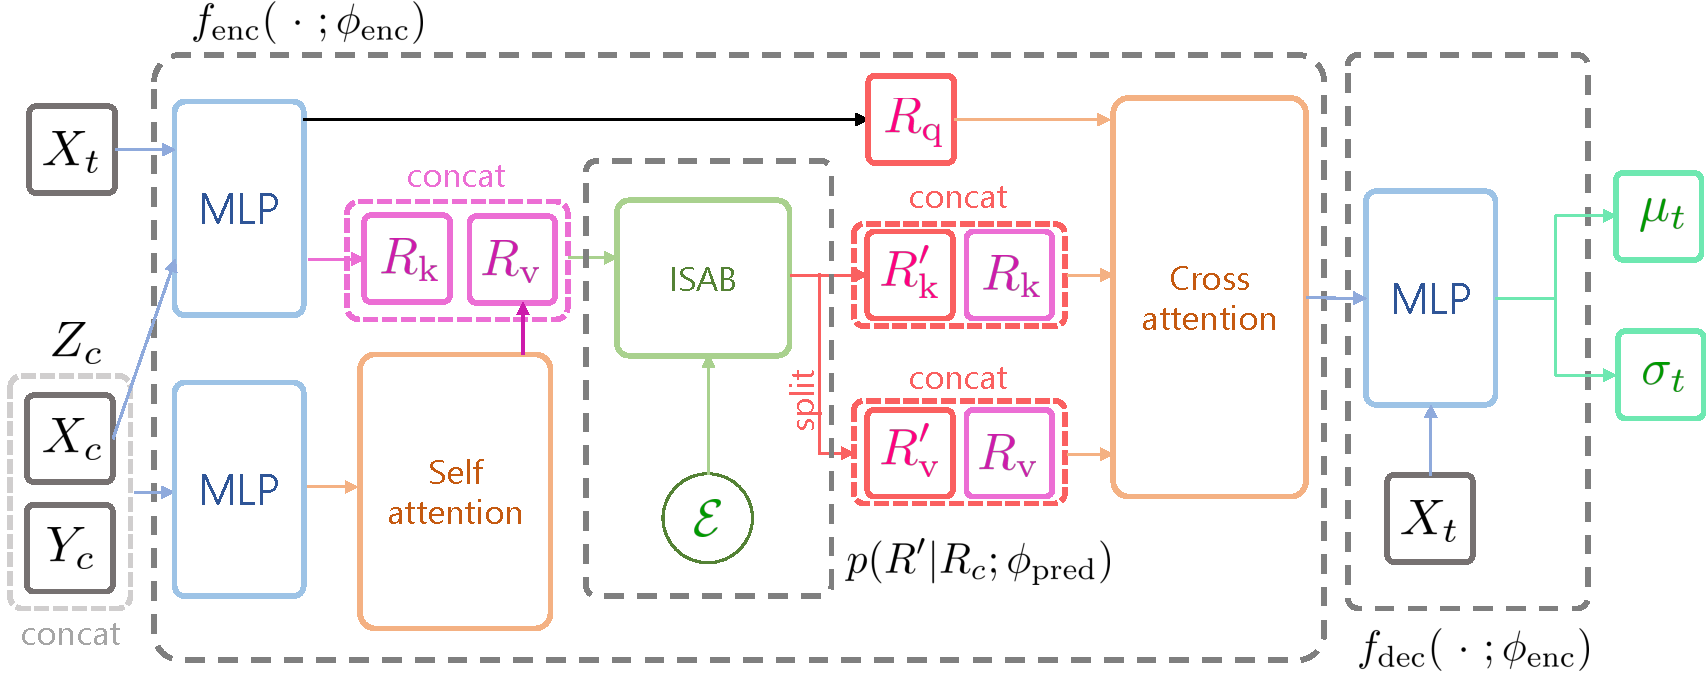
\includegraphics[width = \linewidth]{figure/main_concept_mpanp.pdf}
    \caption{Concept figure of our feature generating model applied to \gls{canp}~\citep{kim2018attentive}. Here we sample $\epsilon$ from a simple distribution (e.g. Gaussian). We generate key feature $R_k'$ and value feature $R_v'$ for cross attention layer which are corresponding to pseudo context data. We use generator as one layer \gls{isab}~\citep{lee2019set} in our experiment.
    %\ed{This figure is awesome!!}}
    }
    \label{figure/main_concept_mpanp}
\end{figure}

In this section, we summarize the model architectures which we used in experiments.
Here, we only present simplified structures for each model.
To see exact computation procedures for \glspl{bnp}, please refer to \citet{lee2020bootstrapping}. \cref{figure/main_concept_mpanp} shows our method applying to \gls{canp} model~\citep{kim2018attentive}.
% To see exact computation procedures for \glspl{bnp} and \glspl{neubnp}, please refer to \citet{lee2020bootstrapping} and \citet{lee2022neural} respectively.

%%%%%%%%%%%%%%%%%%%%%%%%%%%%%%%%%%%%%%%%%%%%%%%%%%
\subsection{Modules}

\paragraph{Linear Layer} $\Lin(d_{\In},d_{\out})$ denotes the linear transformation of the input with dimension $d_{\In}$ into the output with dimension $d_{\out}$.
\paragraph{Multi-Layer Perceptron} $\MLP(n_l, d_{\In}, d_{\hid}, d_{\out})$ denotes a multi-layer perceptron with the structure:
\begin{align*}
    \MLP(n_l, d_{\In}, d_{\hid}, d_{\out}) = \Lin(d_{\hid}, d_{\out})\circ(\ReLU\circ\Lin(d_{\hid},d_{\hid}))^{n_l-2}\circ\ReLU\circ\Lin(d_{\In},d_{\hid}),
\end{align*}
where $\ReLU$ denotes the element-wise Rectified Linear Unit (ReLU) activation function.
\paragraph{Multi-Head Attention} $\MHA(n_{\head}, d_{\out})(Q,K,V)$ denotes a multi-head attention~\citep{vaswani2017attention} with $n_{\head}$ heads which takes input as $(Q,K,V)$ and outputs the feature with dimension $d_{\out}$.
The actual computation of $\MHA(n_{\head}, d_{\out})(Q,K,V)$ can be written as follows:
\begin{align*}
    (Q_i')_{i=1}^{n_\head} &= \spl(\Lin(d_q,d_\out)(Q), n_\head)\\
    (K_i')_{i=1}^{n_\head} &= \spl(\Lin(d_k,d_\out)(K), n_\head)\\
    (V_i')_{i=1}^{n_\head} &= \spl(\Lin(d_v,d_\out)(V), n_\head)\\
    H &= \concat([\softmax(Q_i'K_i'^\top/\sqrt{d_\out})V_i']_{i=1}^{n_\head})\\
    O &= \LN(Q'+H)\\
    \MHA(n_\head,d_\out)(Q,K,V) &= \LN(O+\ReLU(\Lin(d_\out,d_\out)(O)))
\end{align*}
where $(d_q, d_k, d_v)$ denotes the dimension of $Q,K,V$ respectively, $\spl$ and $\concat$ are the splitting and concatenating $A$ in the feature dimension respectively, and $\LN$ denotes the layer normalization~\citep{ba2016layer}.
\paragraph{Self-Attention} $\SA(n_\head, d_\out)$ denotes a self-attention module which is simply computed as $\SA(n_\head, d_\out)(X) = \MHA(n_\head, d_\out)(X,X,X)$.
\paragraph{Multi-head Attention Block} $\MAB(n_\head, d_\out)$ denotes a multi-head attention block module~\citep{lee2019set} which is simply computed as $\MAB(n_\head, d_\out)(X,Y) = \MHA(n_\head, d_\out)(X,Y,Y)$.
\paragraph{Induced Set Attention Block} $\ISAB(n_\head, d_\out)$ denotes a induced set attention block~\citep{lee2019set} which constructed with two stacked $\MAB$ layers.
The actual computation of $\ISAB(n_\head, d_\out)(X,Y)$ can be written as follows:
\begin{align*}
    H &= \MAB(n_\head, d_\out)(Y, X)\\
    \ISAB(n_\head, d_\out)(X,Y) &= \MAB(n_\head, d_\out)(X, H).
\end{align*}

%%%%%%%%%%%%%%%%%%%%%%%%%%%%%%%%%%%%%%%%%%%%%%%%%%
\subsection{\texorpdfstring{\gls{cnp}, \gls{np}, \gls{bnp}, \gls{neubnp} and \gls{mpnp}}{CNP, NP, BNP, NeuBNP, and MPNP}}

\paragraph{Encoder}
The models only with a deterministic encoder (\gls{cnp}, \gls{bnp}, \gls{mpnp}) use the following structure:
\begin{align*}
    r_c &= \frac{1}{|c|} \sum_{i \in c} \MLP(n_l=5, d_{\In}=d_z, d_{\hid}=128, d_{\out}=128)(z_i), \\
    f_\text{enc}(Z_c) &= r_c.
\end{align*}
For the \gls{mpnp}, $f_\enc(Z_c)$ changes into $\concat([r_c,r_c'])$ where $r_c'$ is the feature of the pseudo context data generated from generator in paragraph \textbf{Generator}.
The model also with a latent encoder (\gls{np}) uses:
\begin{align*}
    r_c &= \frac{1}{|c|} \sum_{i \in c} \MLP(n_l=5, d_{\In}=d_z, d_{\hid}=128, d_{\out}=128)(z_i), \\
    (m_c, \log s_c) &= \frac{1}{|c|} \sum_{i \in c} \MLP(n_l=2, d_{\In}=d_z, d_{\hid}=128, d_{\out}=128 \times 2)(z_i), \\
    s_c &= 0.1 + 0.9 \cdot \text{softplus}(\log s_c), \\
    h_c &= \calN(m_c, s^2_c I_h), \\
    f_\text{enc}(Z_c) &= [r_c; h_c],
\end{align*}
where $d_z = d_x + d_y$ denotes the data dimension.
Data dimensions vary through tasks, $d_x=1, d_y=1$ for 1D regression tasks, $d_x=2, d_y=1$ for MNIST image completion task,  $d_x=2, d_y=3$ for SVHN and CelebA image completion tasks, and $d_x=1, d_y=2$ for Lotka Volterra task.

\paragraph{Adaptation Layer}
\gls{bnp} uses additional adaptation layer to combine bootstrapped representation and the base representation. This can be done with a simple linear layer
\[
    \tilde{r}_c = \Lin(d_{\hid}=128, d_{\hid}=d_x+128)(\tilde{r}_c^{(pre)}).
\]

\paragraph{Decoder}
All models use a single MLP as a decoder.
The models except \gls{np} uses the following structure:
\begin{align*}
    (\mu, \log \sigma) &= \MLP(n_l=3, d_{\In}=d_x + 128, d_{\hid}=128, d_{\out}=2)(\concat([x,r_c])) \\
    \sigma &= 0.1 + 0.9 \cdot \text{softplus}(\log \sigma), \\
    f_\text{dec}(x, r_c) &= (\mu, \sigma),
\end{align*}
and \gls{np} uses:
\begin{align*}
    (\mu, \log \sigma) &= \MLP(n_l=3, d_{\In}=d_x + 128 \times 2, d_{\hid}=128, d_{\out}=2)(\concat([x,r_c,h_c])) \\
    \sigma &= 0.1 + 0.9 \cdot \text{softplus}(\log \sigma), \\
    f_\text{dec}(x, r_c, h_c) &= (\mu, \sigma).
\end{align*}


\paragraph{Generator}
\gls{mpnp} use a single $\ISAB$ module as a generator. The $\ISAB$ uses the following structure: 
\begin{align*}
    \epsilon &= \concat([\epsilon_i]_{i=1}^{n_\gen})\\
    r_c' &= \ISAB(n_\head=8, d_\out=128)(\epsilon,r_c)\\
    f_\gen(r_c) &= r_c'
\end{align*}
where $\epsilon_i$s are i.i.d. sampled from Gaussian distribution with dimension 128 and $n_\gen$ denotes a number of pseudo context data.

%%%%%%%%%%%%%%%%%%%%%%%%%%%%%%%%%%%%%%%%%%%%%%%%%%
\subsection{\texorpdfstring{\gls{canp}, \gls{anp}, \gls{banp} and \gls{mpanp}}{CANP, ANP, BANP, NeuBANP, and MPANP}}

\paragraph{Encoder}
The models only with a deterministic encoder (\gls{canp}, \gls{banp}, \gls{neubanp} and \gls{mpanp}) use the following structure:
\begin{align*}
    r_q &= \MLP(n_l=5, d_{\In}=d_x, d_{\hid}=128, d_{\out}=128)(X), \\
    r_k &= \MLP \qquad \qquad \qquad \qquad '' \qquad \qquad \qquad  \qquad \ (X_c), \\
    r_v^{(\text{pre})} &= \MLP(n_l=5, d_{\In}=d_z, d_{\hid}=128, d_{\out}=128)(X_c), \\
    r_v &= \SA(n_\head=8, d_\out=128)(r_v^{(\text{pre})}), \\
    r_c &= \MHA(n_\head=8, d_\out=128)(r_q, r_k, r_v), \\
    f_\text{enc}(Z_c) &= r_c.
\end{align*}
For the \gls{mpanp}, $f_\enc(Z_c)$ changes into 
\begin{align*}
    r_c &= \MHA(n_\head=8, d_\out=128)(r_q, \concat([r_k,r_k']), \concat([r_v,r_v'])),\\
    f_\enc &= r_c,
\end{align*} where $r_k'$ and $r_v'$ are the key and value features of the pseudo context data generated from generator in paragraph \textbf{Generator}.

\gls{anp} constructed as:
\begin{align*}
    r_q &= \MLP(n_l=5, d_{\In}=d_x, d_{\hid}=128, d_{\out}=128)(X), \\
    r_k &= \MLP \qquad \qquad \qquad \qquad '' \qquad \qquad \qquad  \qquad \ (X_c), \\
    r_v' &= \MLP(n_l=5, d_{\In}=d_z, d_{\hid}=128, d_{\out}=128)(X_c), \\
    r_v &= \SA(n_\head=8, d_\out=128)(r_v'), \\
    r_c &= \MHA(n_\head=8, d_\out=128)(r_q, r_k, r_v), \\
    h_i' &= \MLP(n_l=2, d_{\In}=d_z, d_{\hid}=128, d_{\out}=128 \times 2)(z_i), \\
    h_i &= \SA(n_\head=8, d_\out=128)(h_i'), \\
    (m_c, \log s_c) &= \frac{1}{|c|} \sum_{i \in c} h_i, \\
    s_c &= 0.1 + 0.9 \cdot \text{softplus}(\log s_c), \\
    h_c &= \calN(m_c, s^2_c I_h), \\
    f_\text{enc}(Z_c) &= [r_c; h_c].
\end{align*}
Note that $r_q$ and $r_k$ are from the same \MLP. 

\paragraph{Adaptation Layer}
Like \gls{bnp}, \gls{banp} also uses adaptation layer with same structure to combine bootstrapped representations.

\paragraph{Decoder}
All models use the same decoder structure as their non-attentive counterparts.

\paragraph{Generator}
\gls{mpanp} use a single $\ISAB$ module as a generator. The $\ISAB$ uses the following structure: 
\begin{align*}
    \epsilon &= \concat([\epsilon_i]_{i=1}^{n_\gen})\\
    (r_k',r_v') &= \ISAB(n_\head=8, d_\out=256)(\epsilon,\concat([r_k,r_v]))\\
    f_\gen(r_k,r_v) &= (r_k',r_v')
\end{align*}
where $\epsilon_i$s are i.i.d. sampled from Gaussian distribution with dimension 256 and $n_\gen$ denotes a number of pseudo context data.

%%%%%%%%%%%%%%%%%%%%%%%%%%%%%%%%%%%%%%%%%%%%%%%%%%
\section{Additional Experiments}
\label{app:sec:additional_experiments}
%%%%%%%%%%%%%%%%%%%%%%%%%%%%%%%%%%%%%%%%%%%%%%%%%%
\subsection{1D Regression}
\label{app:sec:additional_experiments:1dregression}

\begin{table}[t]
\centering
\setlength{\tabcolsep}{0.3em}
\caption{Test results for 1D regression tasks on RBF, Matern, Periodic, and $t$-noise. `Context' and `Target' respectively denote context and target log-likelihood values, and `Task' denotes the task log-likelihood. All values are averaged over four seeds.}
\label{table/app_gp_inf_full}
\resizebox{\linewidth}{!}{
\begin{tabular}{lrrrrrrrrrrrr}
\toprule
      & \multicolumn{3}{c}{RBF} & \multicolumn{3}{c}{Matern} & \multicolumn{3}{c}{Periodic} & \multicolumn{3}{c}{$t$-noise} \\
\cmidrule(lr){2-4}\cmidrule(lr){5-7}\cmidrule(lr){8-10}\cmidrule(lr){11-13}
Model & Context & Target & Task & Context & Target & Task & Context & Target & Task & Context & Target & Task \\
\midrule
CNP & 
 1.096$\spm{0.023}$ &  0.515$\spm{0.018}$ &  0.796$\spm{0.020}$ &
 1.031$\spm{0.010}$ &  0.347$\spm{0.006}$ &  0.693$\spm{0.008}$ &
-0.120$\spm{0.020}$ & -0.729$\spm{0.004}$ & -0.363$\spm{0.012}$ &
 0.032$\spm{0.014}$ & -0.816$\spm{0.032}$ & -0.260$\spm{0.012}$ \\
NP & 
 1.022$\spm{0.005}$ &  0.498$\spm{0.003}$ &  0.748$\spm{0.004}$ &
 0.948$\spm{0.006}$ &  0.337$\spm{0.005}$ &  0.641$\spm{0.005}$ &
-0.267$\spm{0.024}$ & \textBF{-0.668}$\spm{0.006}$ & -0.441$\spm{0.013}$ &
 \textBF{0.201}$\spm{0.025}$ & -0.333$\spm{0.078}$ & \textBF{-0.038}$\spm{0.026}$ \\
BNP & 
 1.112$\spm{0.003}$ &  0.588$\spm{0.004}$ &  0.841$\spm{0.003}$ &
 1.057$\spm{0.009}$ &  0.418$\spm{0.006}$ &  0.741$\spm{0.007}$ &
-0.106$\spm{0.017}$ & -0.705$\spm{0.001}$ & -0.347$\spm{0.010}$ &
-0.009$\spm{0.032}$ & -0.619$\spm{0.191}$ & -0.217$\spm{0.036}$ \\
\textBF{MPNP (ours)} & 
 \textBF{1.189}$\spm{0.005}$ &  \textBF{0.675}$\spm{0.003}$ &  \textBF{0.911}$\spm{0.003}$ &
 \textBF{1.123}$\spm{0.005}$ &  \textBF{0.481}$\spm{0.007}$ &  \textBF{0.796}$\spm{0.005}$ &
 \textBF{0.205}$\spm{0.020}$ & \textBF{-0.668}$\spm{0.008}$ & \textBF{-0.171}$\spm{0.013}$ &
 0.145$\spm{0.017}$ & \textBF{-0.329}$\spm{0.025}$ & -0.061$\spm{0.012}$ \\
\midrule
CANP & 
 1.304$\spm{0.027}$ &  0.847$\spm{0.005}$ &  1.036$\spm{0.020}$ &
 1.264$\spm{0.041}$ &  0.662$\spm{0.013}$ &  0.937$\spm{0.031}$ &
 0.527$\spm{0.106}$ & -0.592$\spm{0.002}$ &  0.010$\spm{0.069}$ &
 0.410$\spm{0.155}$ & -0.577$\spm{0.022}$ & -0.008$\spm{0.098}$ \\
ANP & 
 \textBF{1.380}$\spm{0.000}$ &  0.850$\spm{0.007}$ &  1.090$\spm{0.003}$ &
 \textBF{1.380}$\spm{0.000}$ &  0.663$\spm{0.004}$ &  1.019$\spm{0.002}$ &
 0.583$\spm{0.011}$ & -1.019$\spm{0.023}$ &  0.090$\spm{0.004}$ &
 0.836$\spm{0.071}$ & -0.415$\spm{0.131}$ &  0.374$\spm{0.034}$ \\
BANP & 
 \textBF{1.380}$\spm{0.000}$ &  0.846$\spm{0.001}$ &  1.088$\spm{0.000}$ &
 \textBF{1.380}$\spm{0.000}$ &  0.662$\spm{0.005}$ &  1.018$\spm{0.002}$ &
 \textBF{1.354}$\spm{0.006}$ & -0.496$\spm{0.005}$ &  \textBF{0.634}$\spm{0.005}$ &
 0.646$\spm{0.042}$ & -0.425$\spm{0.050}$ &  0.270$\spm{0.033}$ \\
\textBF{MPANP (ours)} & 
 1.379$\spm{0.000}$ &  \textBF{0.881}$\spm{0.003}$ &  \textBF{1.102}$\spm{0.001}$ &
 \textBF{1.380}$\spm{0.000}$ &  \textBF{0.692}$\spm{0.003}$ &  \textBF{1.029}$\spm{0.001}$ &
 1.348$\spm{0.005}$ & \textBF{-0.494}$\spm{0.007}$ &  0.630$\spm{0.005}$ &
 \textBF{0.842}$\spm{0.062}$ & \textBF{-0.332}$\spm{0.026}$ &  \textBF{0.384}$\spm{0.041}$ \\
\bottomrule
\end{tabular}}
\end{table}

\paragraph{Full results for~\cref{table/main_gp_inf}}
We provide the full test results for 1D regression tasks including context, target, and task log-likelihood values in~\cref{table/app_gp_inf_full}.

\paragraph{Increasing the encoder size of baselines}
\begin{table}[t]
\centering
\caption{Further comparisons with baselines with increased number of parameters. `Context' and `Target' respectively denote context and target log-liklihood values, and `Task' denotes the task log-likelihood. All values are averaged over four seeds.}
\label{table/app_gp_inf_sizeup}
\resizebox{\linewidth}{!}{
\begin{tabular}{lrrrrrrr}
\toprule
      & & \multicolumn{3}{c}{RBF} & \multicolumn{3}{c}{Matern} \\
\cmidrule(lr){3-5}\cmidrule(lr){6-8}
Model & \# Params & Context & Target & Task & Context & Target & Task \\
\midrule
CNP & 264 K & 
1.096$\spm{0.008}$ & 0.517$\spm{0.007}$ & 0.797$\spm{0.007}$ &
1.017$\spm{0.021}$ & 0.340$\spm{0.012}$ & 0.681$\spm{0.017}$ \\
NP  & 274 K & 
1.026$\spm{0.004}$ & 0.501$\spm{0.003}$ & 0.752$\spm{0.003}$ &
0.948$\spm{0.005}$ & 0.334$\spm{0.002}$ & 0.640$\spm{0.003}$ \\
BNP & 261 K & 
1.115$\spm{0.007}$ & 0.591$\spm{0.005}$ & 0.843$\spm{0.006}$ &
1.051$\spm{0.007}$ & 0.416$\spm{0.005}$ & 0.736$\spm{0.005}$ \\
\textBF{MPNP (ours)} & 266 K &
\textBF{1.189}$\spm{0.005}$ & \textBF{0.675}$\spm{0.003}$ & \textBF{0.911}$\spm{0.003}$ &
\textBF{1.123}$\spm{0.005}$ & \textBF{0.481}$\spm{0.007}$ & \textBF{0.796}$\spm{0.005}$ \\
\midrule
CANP & 868 K & 
1.305$\spm{0.007}$ & 0.844$\spm{0.006}$ & 1.035$\spm{0.005}$ &
1.278$\spm{0.013}$ & 0.663$\spm{0.006}$ & 0.947$\spm{0.008}$ \\
ANP  & 877 K & 
\textBF{1.380}$\spm{0.000}$ & 0.858$\spm{0.002}$ & 1.093$\spm{0.001}$ &
\textBF{1.380}$\spm{0.000}$ & 0.668$\spm{0.006}$ & 1.020$\spm{0.002}$ \\
BANP & 885 K & 
1.379$\spm{0.001}$ & 0.839$\spm{0.015}$ & 1.085$\spm{0.007}$ &
1.376$\spm{0.005}$ & 0.652$\spm{0.032}$ & 1.012$\spm{0.014}$ \\
\textBF{MPANP (ours)} & 877 K &
1.379$\spm{0.000}$ & \textBF{0.881}$\spm{0.003}$ & \textBF{1.102}$\spm{0.001}$ &
\textBF{1.380}$\spm{0.000}$ &  \textBF{0.692}$\spm{0.003}$ &  \textBF{1.029}$\spm{0.001}$ \\
\bottomrule
\end{tabular}}
\end{table}

Since the generator increases the size of the encoder in \glspl{mpnp}, one can claim that the performance gain of \glspl{mpnp} may come from the increased model size. To verify this, we increased the hidden dimensions of the encoder of baselines and compared them with ours. The results displayed in~\cref{table/app_gp_inf_sizeup} further clarify that ours still outperforms the baselines even when the number of parameters gets in line.


\subsection{High-D Regression}
% \paragraph{Settings}
We conducted additional experiments on the synthetic high-dimensional regression data (i.e., generating one-dimensional y from four-dimensional x with RBF kernel). Here we used the same model structures with the 1D regression task except for the input layer, and the same settings for the RBF kernel with 1D regression except for $l\sim \text{Unif}(0.5, 3.0)$. We fixed the base learning rate to $0.00015$ for all models throughout the high-dimensional regression experiments.


% \paragraph{Results}
\cref{table/app_high_d} clearly shows our \glspl{mpnp} still outperform baselines for log-likelihood values we measured.


\begin{table}[t]
\centering

\caption{Test results for 4D regression tasks on RBF. `Context' and `Target' respectively denote context and target log-likelihood values, and `Task' denotes the task log-likelihood. All values are averaged over four seeds.}
\label{table/app_high_d}

\begin{tabular}{lrrr}
\toprule
& \multicolumn{3}{c}{RBF}  \\
\cmidrule(lr){2-4}
Model & Context & Target & Task  \\
\midrule
CNP & 0.572$\spm{0.003}$ &  0.265$\spm{0.002}$ &  0.410$\spm{0.003}$ \\
NP  & 0.568$\spm{0.009}$ &  0.267$\spm{0.004}$ &  0.407$\spm{0.007}$ \\
BNP & 0.621$\spm{0.015}$ &  0.323$\spm{0.008}$ &  0.467$\spm{0.013}$ \\
\textBF{MPNP (ours)} & 
\textBF{0.820}$\spm{0.002}$ & \textBF{0.441}$\spm{0.004}$ & \textBF{0.633}$\spm{0.004}$ \\
\midrule
CANP & 0.957$\spm{0.005}$ &  0.585$\spm{0.006}$ &  0.743$\spm{0.005}$  \\
ANP & 1.357$\spm{0.006}$ &  0.320$\spm{0.014}$ &  0.890$\spm{0.007}$  \\
BANP & \textBF{1.380}$\spm{0.000}$ &  0.549$\spm{0.006}$ &  1.013$\spm{0.002}$  \\
\textBF{MPANP (ours)} & 1.379$\spm{0.000}$ &  \textBF{0.645}$\spm{0.007}$ &  \textBF{1.046}$\spm{0.002}$ \\
\bottomrule
\end{tabular}
\end{table}


%%%%%%%%%%%%%%%%%%%%%%%%%%%%%%%%%%%%%%%%%%%%%%%%%%
\subsection{Image Completion}
\label{app:sec:additional_experiments:imagecompletion}

\begin{figure}[t]
    \centering
    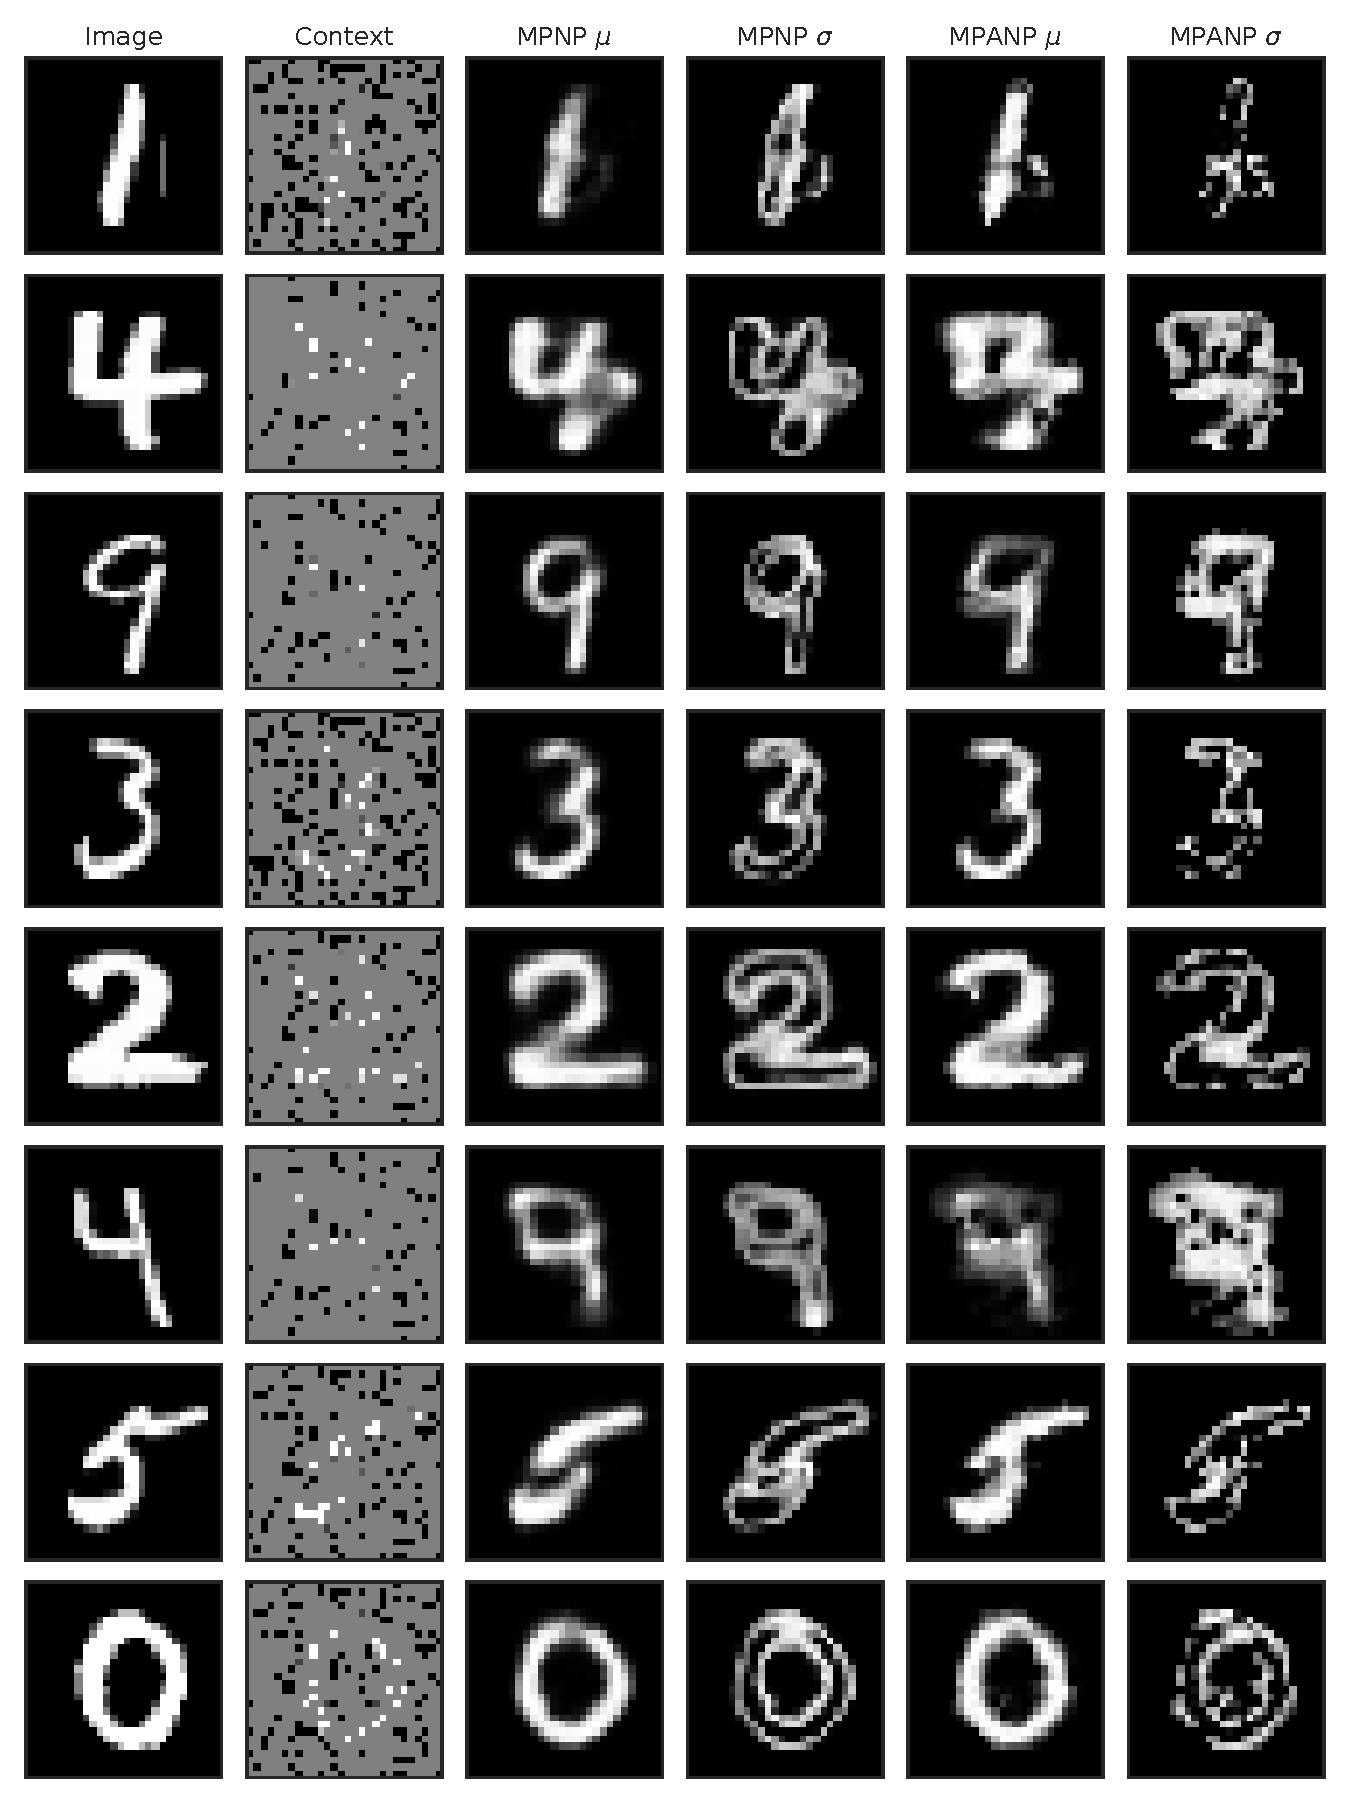
\includegraphics[width = \textwidth]{figure/app_visualize_mnist.pdf}
    \caption{Predicted mean and standard deviation of image pixels by trained \glspl{mpnp} with MNIST dataset. The first column shows the real image from test dataset. The second column shows the context dataset which given to the models. The third and the forth columns show the predicted mean and standard deviation from the \gls{mpnp} respectively. The fifth and the sixth columns show the predicted mean and standard deviation from the \gls{mpanp}.} 
    \label{figure/app_visualize_mnist}
\end{figure}

\begin{figure}
    \centering
    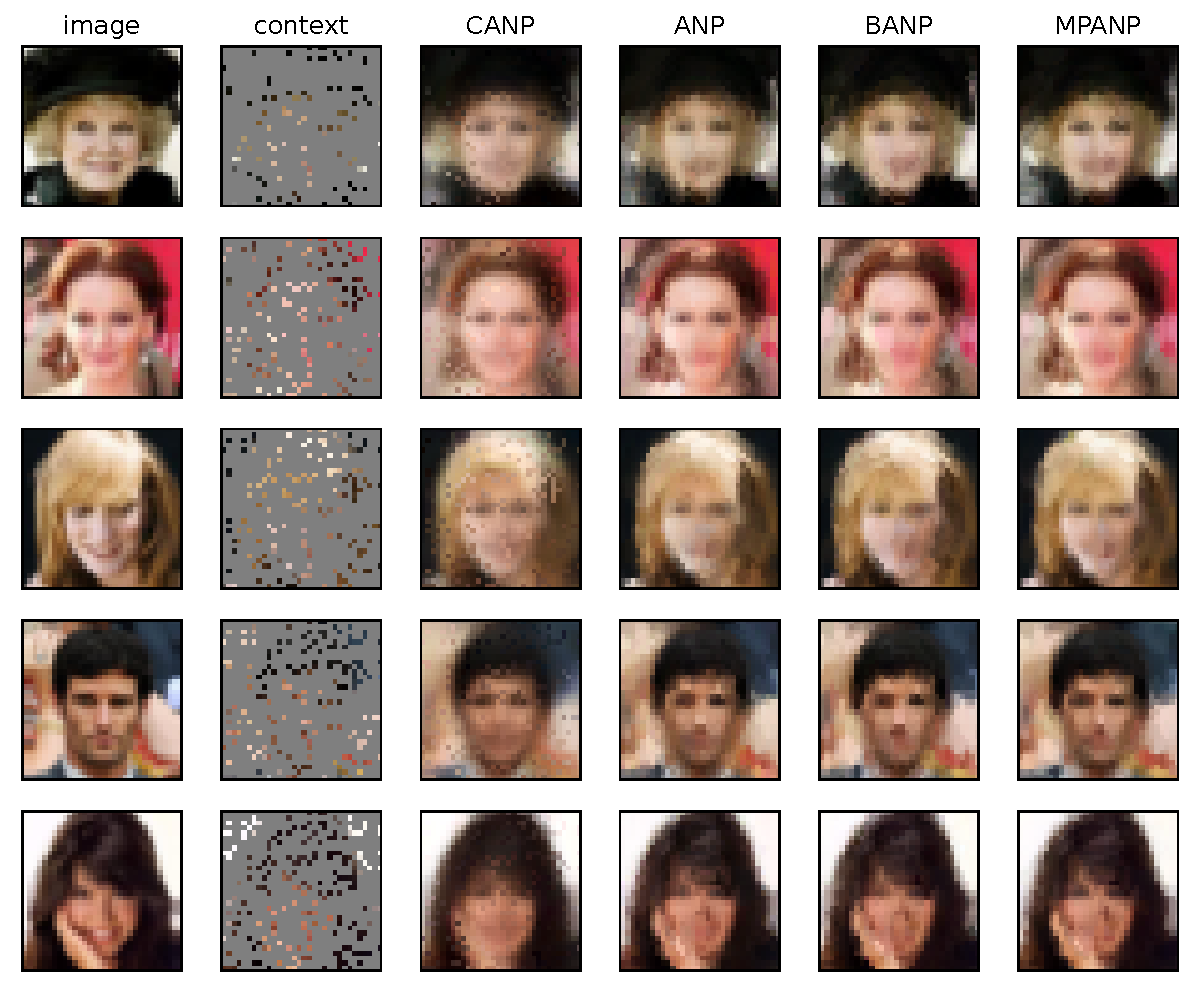
\includegraphics[width=\linewidth]{figure/app_visualize_celeba.pdf}
    \caption{Predicted mean of image pixels by trained \gls{canp}, \gls{anp}, \gls{banp} and \gls{mpanp} model. (Column 1) Here we can see the 5 ground truth real image from the test dataset. (Column 2) The context set which given to the models. (Column 3-6) The predicted mean of image pixels by each models.}
    \label{figure/app_visualize_celeba}
\end{figure}


\paragraph{MNIST}
We provide some completed MNIST images in~\cref{figure/app_visualize_mnist}. It shows that both \gls{mpnp} and \gls{mpanp} successfully fill up the remaining parts of the image for a given context and capture the uncertainties as predictive variances.

\paragraph{CelebA}
We also present five examples from the CelebA dataset in~\cref{figure/app_visualize_celeba}. It shows that \gls{mpanp} provides perceptually reasonable predictions even for complex three-channel images.

% In this section, we presents some examples of the visualizations of completed images along with the uncertainties in terms of predictive variances.
% We report 8 samples for the MNIST dataset.
% In \cref{figure/app_visualize_mnist}, we report the results for the image completion with MNIST test dataset.
% Here we can see that both the \gls{mpnp} and the \gls{mpanp} well complete the remain parts of the image and well capture the uncertainties in terms of predictive variances.

%%%%%%%%%%%%%%%%%%%%%%%%%%%%%%%%%%%%%%%%%%%%%%%%%%
\subsection{Bayesian Optimization}
\label{app:sec:additional_experiments:bo}


\begin{figure}
\centering
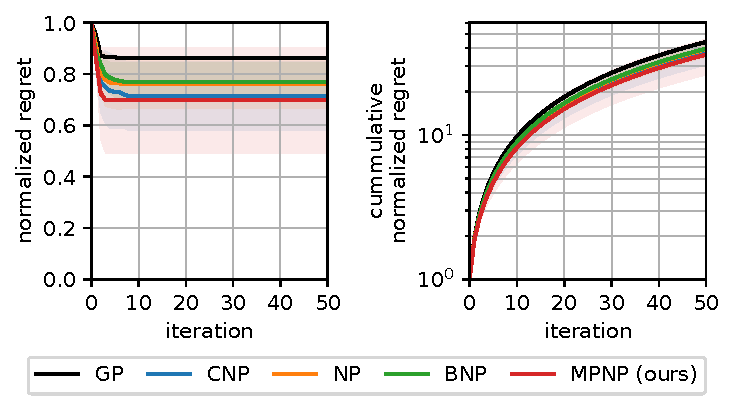
\includegraphics[width=0.49\linewidth]{figure/app_bo_sob_np.pdf}
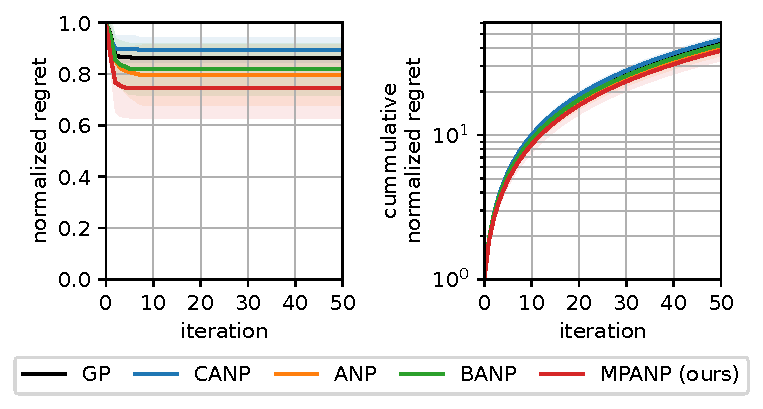
\includegraphics[width=0.49\linewidth]{figure/app_bo_sob_anp.pdf}
\caption{Results for Bayesian optimization on~\citet{sobester2008engineering} function.}
\label{figure/app_bo_sob}
\end{figure}
We provide the results for Bayesian optimization on the~\citet{sobester2008engineering} function in~\cref{figure/app_bo_sob}. Our \glspl{mpnp} consistently outperform baselines as discussed in~\cref{main:sec:experiments:bo}. We also present the visual results for Bayesian optimization in~\cref{figure/app_visualize_bo_np,figure/app_visualize_bo_anp}.

\begin{figure}
\centering
\begin{subfigure}[b]{\textwidth}
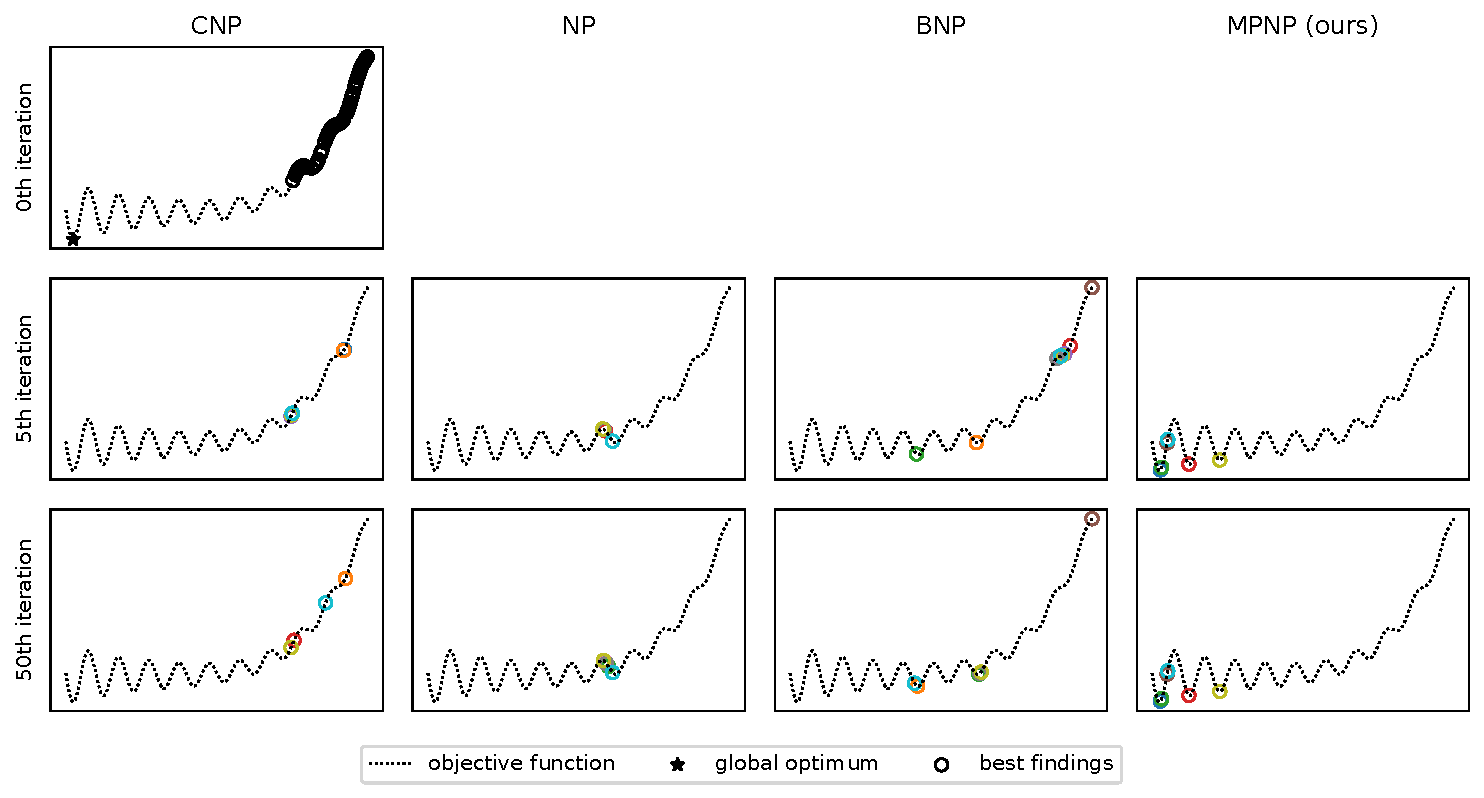
\includegraphics[width=\linewidth]{figure/app_visualize_bo_gram_np.pdf}
\caption{\citet{gramacy2012cases} function}
\end{subfigure}
\bigskip

\begin{subfigure}[b]{\textwidth}
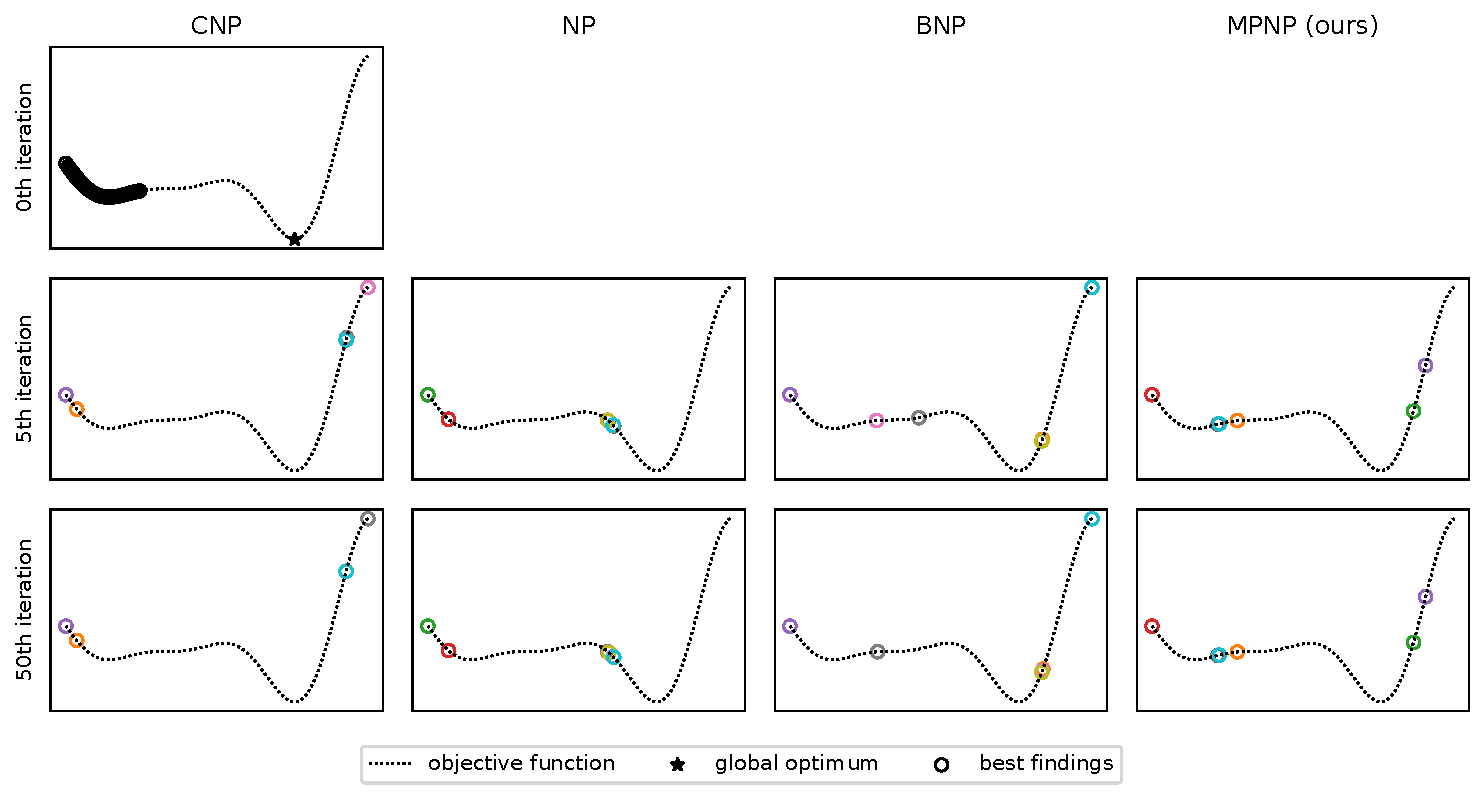
\includegraphics[width=\linewidth]{figure/app_visualize_bo_sob_np.pdf}
\caption{\citet{sobester2008engineering} function}
\end{subfigure}
\caption{It depicts 10 solutions predicted by \gls{cnp}, \gls{np}, \gls{bnp}, and \gls{mpnp}. (a,b) Predicted results for \citet{gramacy2012cases} function and \citet{sobester2008engineering} function, respectively. (Row 1) Black circles indicate the whole initial points. (Row 2) It shows the 10 best solutions predicted by each models after the 5 iterations. (Row 3) It shows the 10 best solutions predicted by each models after the whole iterations.}
\label{figure/app_visualize_bo_np}
\end{figure}

\begin{figure}
\centering
\begin{subfigure}[b]{\textwidth}
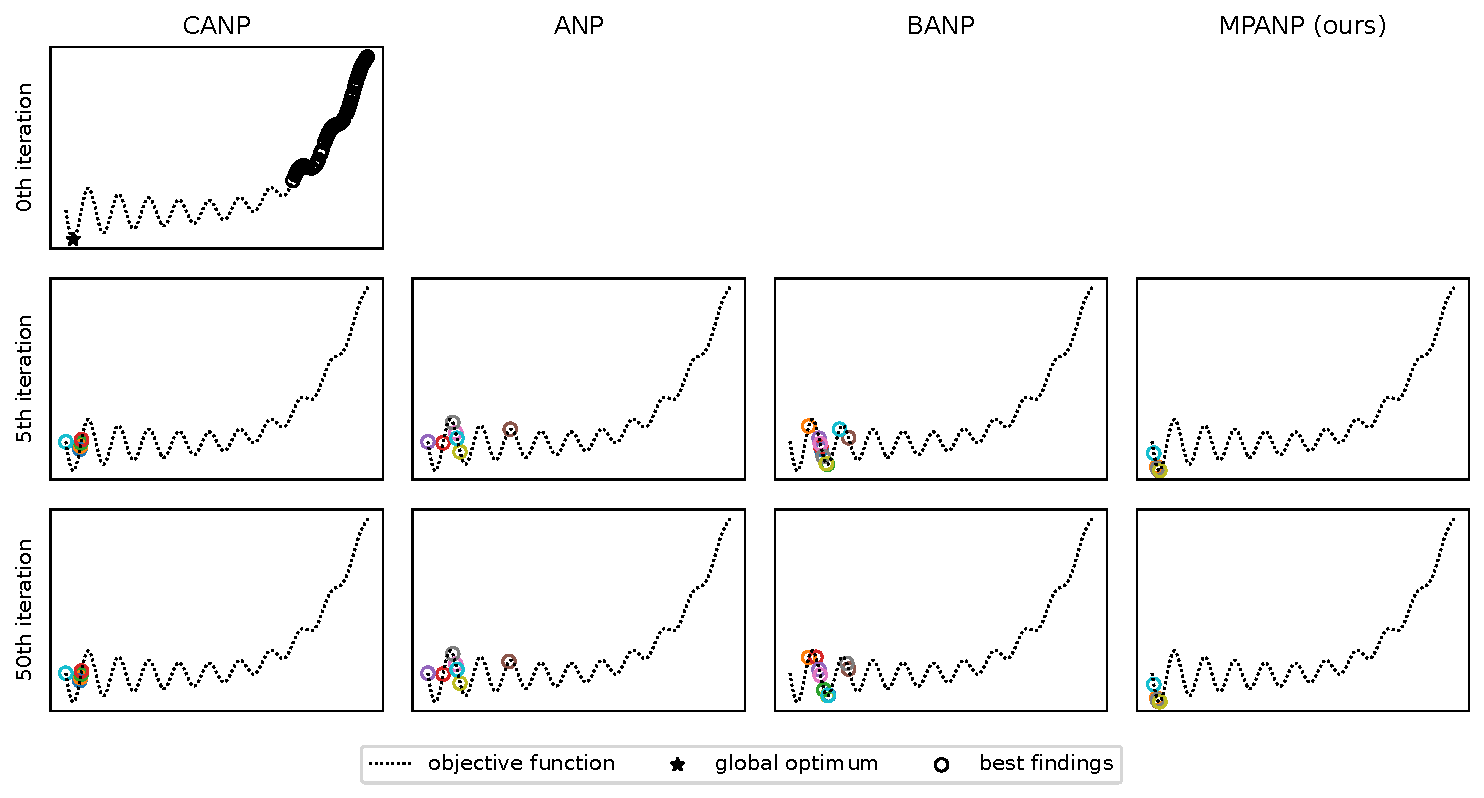
\includegraphics[width=\linewidth]{figure/app_visualize_bo_gram_anp.pdf}
\caption{\citet{gramacy2012cases} function}
\end{subfigure}
\bigskip

\begin{subfigure}[b]{\textwidth}
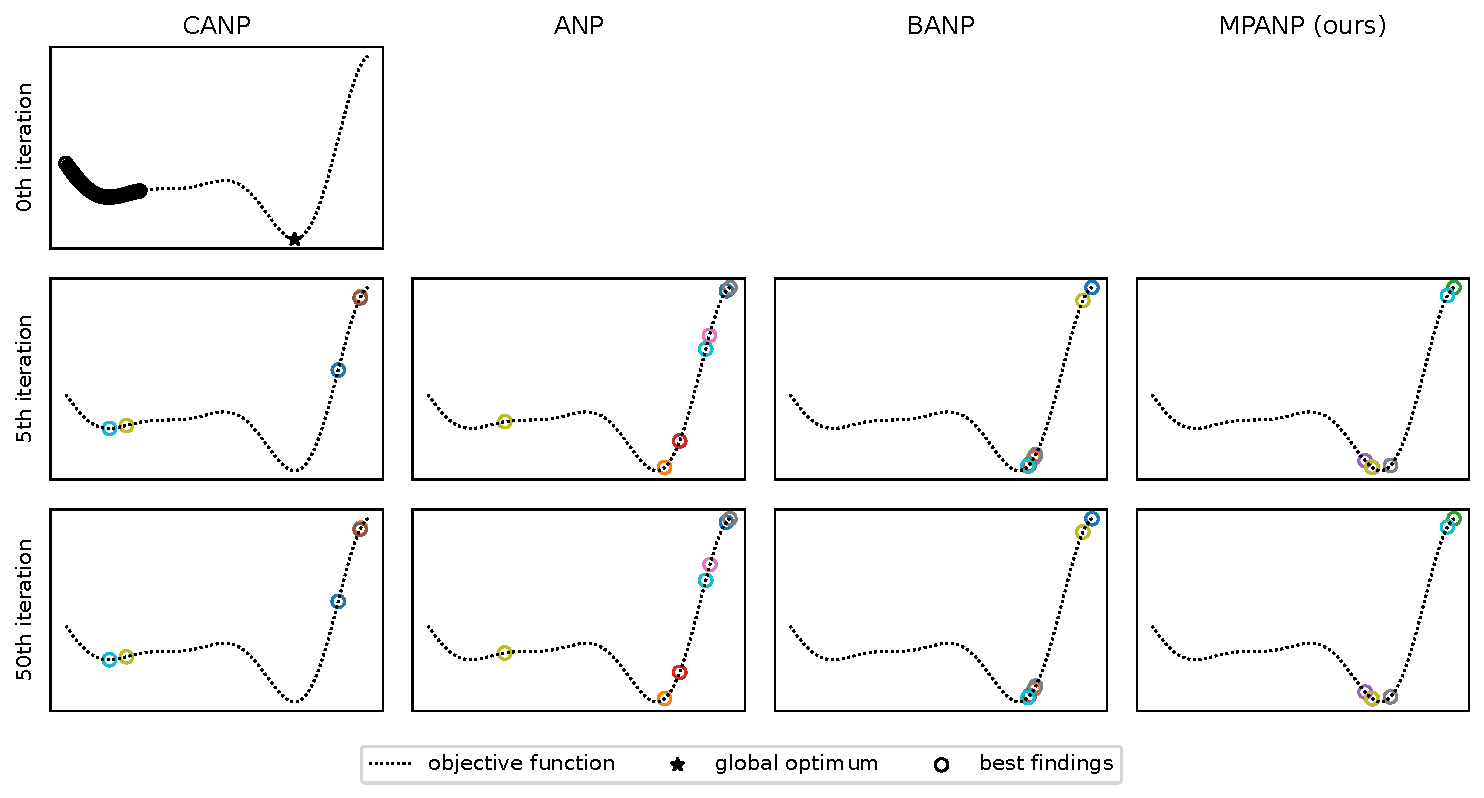
\includegraphics[width=\linewidth]{figure/app_visualize_bo_sob_anp.pdf}
\caption{\citet{sobester2008engineering} function}
\end{subfigure}
\caption{It depicts 10 solutions predicted by \gls{canp}, \gls{anp}, \gls{banp}, and \gls{mpanp}. (a,b) Predicted results for \citet{gramacy2012cases} function and \citet{sobester2008engineering} function, respectively. (Row 1) Black circles indicate the whole initial points. (Row 2) It shows the 10 best solutions predicted by each models after the 5 iterations. (Row 3) It shows the 10 best solutions predicted by each models after the whole iterations.}
\label{figure/app_visualize_bo_anp}
\end{figure}




% Here as the generator increases the size of the encoder in \glspl{mpnp}, we also increase the size of the encoder of the baselines for the fare comparisons. 
% As you can see in \cref{tab:table_gp_inf_eq}, our model still significantly outperforms the baselines.

% \begin{table}[t]
%     \caption{Context and target log likelihood values on data sampled from Gaussian Processes with various kernel. Here we used almost the same number of parameters for models. Performances are measured over 4 seeds.\\}
%     \label{tab:table_gp_inf_eq}
%     \centering
%     \scriptsize
%     \renewcommand{\arraystretch}{0.9}
%     \resizebox{0.95\textwidth}{!}{
%     \begin{tabular}{lrrrrrrrrrrrr}
%         \toprule
%         \multirow{3}{*}{Model} & \multicolumn{2}{r}{RBF}                                   & \multicolumn{2}{r}{Matern}                                & \multicolumn{2}{r}{Periodic}                                & \multicolumn{2}{r}{$t$-noise}                               \\
%                                  \cmidrule(lr){2-3}                                          \cmidrule(lr){4-5}                                          \cmidrule(lr){6-7}                                            \cmidrule(lr){8-9}
%                               & context                     & target                      & context                     & target                      & context                      & target                       & context                      & target                       \\
%         \midrule
% CNP                    &         0.983  $\pm{0.006}$ &         0.298  $\pm{0.006}$ &         0.889  $\pm{0.010}$ &         0.140  $\pm{0.003}$ &         -0.091  $\pm{0.010}$ &         -0.742  $\pm{0.039}$ &         -0.032  $\pm{0.021}$ &         -0.724  $\pm{0.018}$ \\
% NP                     &         0.984  $\pm{0.010}$ &         0.308  $\pm{0.008}$ &         0.876  $\pm{0.004}$ &         0.148  $\pm{0.006}$ &         -0.325  $\pm{0.049}$ &         -0.698  $\pm{0.035}$ &         -0.016  $\pm{0.022}$ &         -0.677  $\pm{0.039}$ \\
% BNP                    &         1.042  $\pm{0.007}$ &         0.371  $\pm{0.003}$ &         0.904  $\pm{0.013}$ &         0.176  $\pm{0.006}$ &         -0.087  $\pm{0.004}$ &         -0.738  $\pm{0.022}$ &         -0.042  $\pm{0.051}$ &         -0.664  $\pm{0.021}$ \\
% % NeuBNP                 &         0.954  $\pm{0.010}$ &         0.284  $\pm{0.004}$ &         0.861  $\pm{0.014}$ &         0.130  $\pm{0.003}$ &         -0.176  $\pm{0.028}$ &         -0.797  $\pm{0.015}$ &         -0.066  $\pm{0.013}$ &         -0.683  $\pm{0.096}$ \\
% MPNP (ours)            & \textBF{1.086} $\pm{0.005}$ & \textBF{0.457} $\pm{0.002}$ & \textBF{1.005} $\pm{0.014}$ & \textBF{0.278} $\pm{0.006}$ & \textBF{-0.017} $\pm{0.013}$ & \textBF{-0.681} $\pm{0.009}$ & \textBF{ 0.119} $\pm{0.025}$ & \textBF{-0.381} $\pm{0.013}$ \\
% \cmidrule(lr){1-1}       \cmidrule(lr){2-3}                                          \cmidrule(lr){4-5}                                          \cmidrule(lr){6-7}                                            \cmidrule(lr){8-9}
% CANP                   &         1.372  $\pm{0.001}$ &         0.625  $\pm{0.005}$ &         1.370  $\pm{0.002}$ &         0.429  $\pm{0.016}$ &          1.157  $\pm{0.051}$ &         -0.748  $\pm{0.037}$ &          0.309  $\pm{0.065}$ &         -0.804  $\pm{0.049}$ \\
% ANP                    &         1.374  $\pm{0.001}$ &         0.648  $\pm{0.016}$ &         1.371  $\pm{0.002}$ &         0.462  $\pm{0.020}$ &          1.191  $\pm{0.054}$ &         -0.709  $\pm{0.024}$ &          0.695  $\pm{0.048}$ &         -0.750  $\pm{0.082}$ \\
% BANP                   &         1.372  $\pm{0.000}$ &         0.653  $\pm{0.014}$ &         1.370  $\pm{0.002}$ &         0.450  $\pm{0.006}$ & \textBF{ 1.243} $\pm{0.083}$ &         -0.647  $\pm{0.028}$ &          0.437  $\pm{0.034}$ &         -0.645  $\pm{0.057}$ \\
% % NeuBANP                &         1.358  $\pm{0.001}$ &         0.661  $\pm{0.003}$ &         1.352  $\pm{0.001}$ &         0.477  $\pm{0.004}$ &          0.721  $\pm{0.018}$ &         -0.790  $\pm{0.007}$ &          0.763  $\pm{0.060}$ &         -0.460  $\pm{0.019}$ \\
% MPANP (ours)           & \textBF{1.374} $\pm{0.000}$ & \textBF{0.698} $\pm{0.007}$ & \textBF{1.373} $\pm{0.001}$ & \textBF{0.501} $\pm{0.005}$ &          1.167  $\pm{0.047}$ & \textBF{-0.628} $\pm{0.027}$ & \textBF{ 0.773} $\pm{0.039}$ & \textBF{-0.446} $\pm{0.057}$ \\
% % CNP                    &         0.964  $\pm{0.006}$ &         0.288  $\pm{0.006}$ &         0.859  $\pm{0.009}$ &         0.124  $\pm{0.011}$ &         -0.139  $\pm{0.007}$ &         -0.742  $\pm{0.011}$ &         -0.012  $\pm{0.021}$ &         -0.760  $\pm{0.025}$ \\
% % NP                     &         0.953  $\pm{0.003}$ &         0.306  $\pm{0.004}$ &         0.842  $\pm{0.015}$ &         0.133  $\pm{0.008}$ &         -0.346  $\pm{0.026}$ &         -0.698  $\pm{0.007}$ &         -0.018  $\pm{0.022}$ &         -0.656  $\pm{0.028}$ \\
% % BNP                    &         1.020  $\pm{0.006}$ &         0.372  $\pm{0.006}$ &         0.929  $\pm{0.008}$ &         0.206  $\pm{0.006}$ &         -0.036  $\pm{0.031}$ &         -0.738  $\pm{0.011}$ &         -0.051  $\pm{0.051}$ &         -0.670  $\pm{0.023}$ \\
% % NeuBNP                 &         0.929  $\pm{0.011}$ &         0.275  $\pm{0.007}$ &         0.834  $\pm{0.008}$ &         0.122  $\pm{0.004}$ &         -0.231  $\pm{0.010}$ &         -0.785  $\pm{0.023}$ &          0.038  $\pm{0.009}$ &         -0.516  $\pm{0.018}$ \\
% % MPNP (ours)            & \textBF{1.086} $\pm{0.005}$ & \textBF{0.457} $\pm{0.002}$ & \textBF{1.005} $\pm{0.014}$ & \textBF{0.278} $\pm{0.006}$ & \textBF{-0.017} $\pm{0.013}$ & \textBF{-0.681} $\pm{0.009}$ & \textBF{ 0.119} $\pm{0.025}$ & \textBF{-0.381} $\pm{0.013}$ \\
% % \cmidrule(lr){1-1}       \cmidrule(lr){2-3}                                          \cmidrule(lr){4-5}                                          \cmidrule(lr){6-7}                                            \cmidrule(lr){8-9}
% % CANP                   &         1.372  $\pm{0.000}$ &         0.611  $\pm{0.008}$ &         1.370  $\pm{0.001}$ &         0.423  $\pm{0.004}$ &          1.168  $\pm{0.051}$ &         -0.747  $\pm{0.037}$ &          0.404  $\pm{0.057}$ &         -1.036  $\pm{0.103}$ \\
% % ANP                    &         1.372  $\pm{0.003}$ &         0.617  $\pm{0.027}$ &         1.372  $\pm{0.001}$ &         0.432  $\pm{0.025}$ & \textBF{1.178}  $\pm{0.054}$ &         -0.719  $\pm{0.024}$ &          0.708  $\pm{0.054}$ &         -0.728  $\pm{0.093}$ \\
% % BANP                   & \textBF{1.374} $\pm{0.001}$ &         0.663  $\pm{0.002}$ &         1.371  $\pm{0.002}$ &         0.472  $\pm{0.003}$ &          0.754  $\pm{0.083}$ &         -0.913  $\pm{0.028}$ &          0.477  $\pm{0.008}$ &         -0.660  $\pm{0.059}$ \\
% % NeuBANP                &         1.357  $\pm{0.002}$ &         0.651  $\pm{0.005}$ &         1.352  $\pm{0.002}$ &         0.473  $\pm{0.007}$ &          0.697  $\pm{0.022}$ &         -0.779  $\pm{0.013}$ &          0.670  $\pm{0.028}$ &         -0.450  $\pm{0.014}$ \\
% % MPANP (ours)           & \textBF{1.374} $\pm{0.000}$ & \textBF{0.698} $\pm{0.007}$ & \textBF{1.373} $\pm{0.001}$ & \textBF{0.501} $\pm{0.005}$ &         1.167 $\pm{0.047}$ & \textBF{-0.628} $\pm{0.027}$ & \textBF{ 0.773} $\pm{0.039}$ & \textBF{-0.446} $\pm{0.057}$ \\
%         \bottomrule
%     \end{tabular}}
% \end{table}
% In this section, we report the experiment results with the baselines with increased number of parameters to match the additional number of parameters introduced for the generator in \glspl{mpnp}.
% Here as the generator increases the size of the encoder in \glspl{mpnp}, we also increase the size of the encoder of the baselines for the fare comparisons. 
% As you can see in \cref{tab:table_gp_inf_eq}, our model still significantly outperforms the baselines.

% \subsection{Finite Training Dataset Other Kernels}
% \begin{figure}[t]
%     \centering
%     % 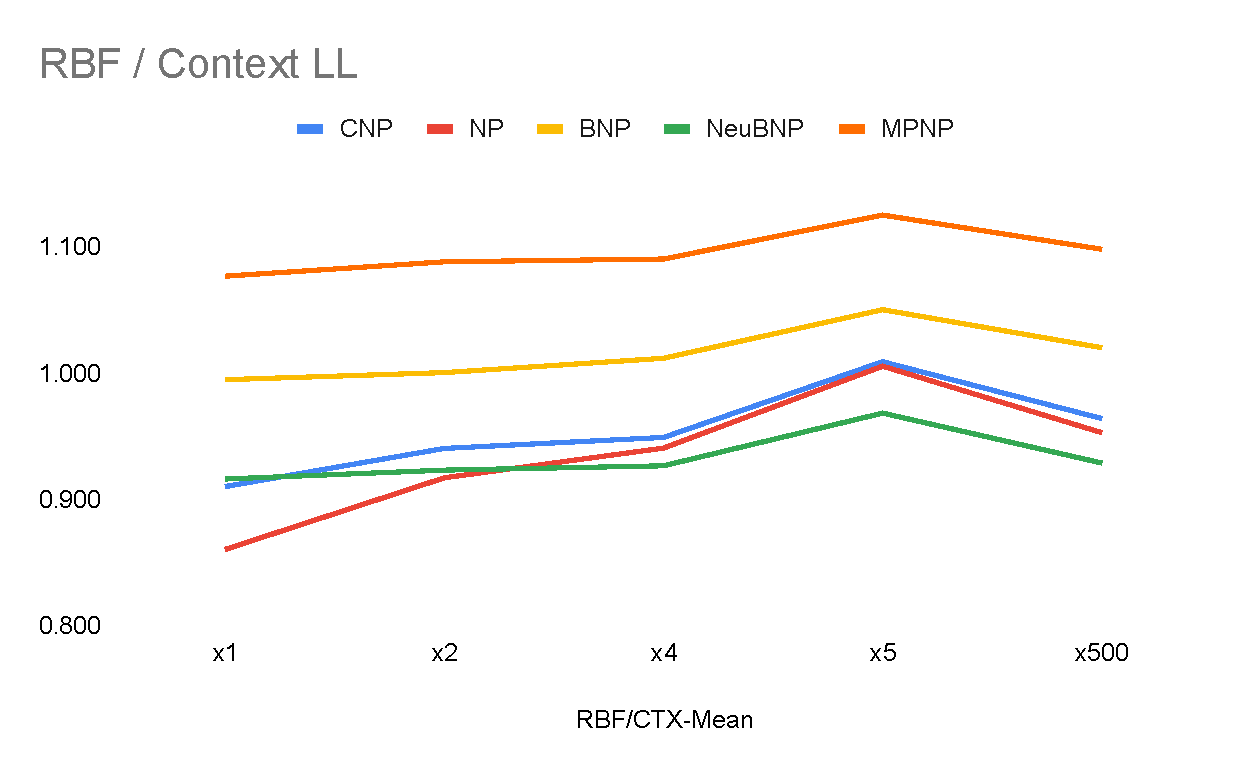
\includegraphics[width=0.24\textwidth]{figure/gp_finite/rbf_ctx_cnps.pdf}
%     % 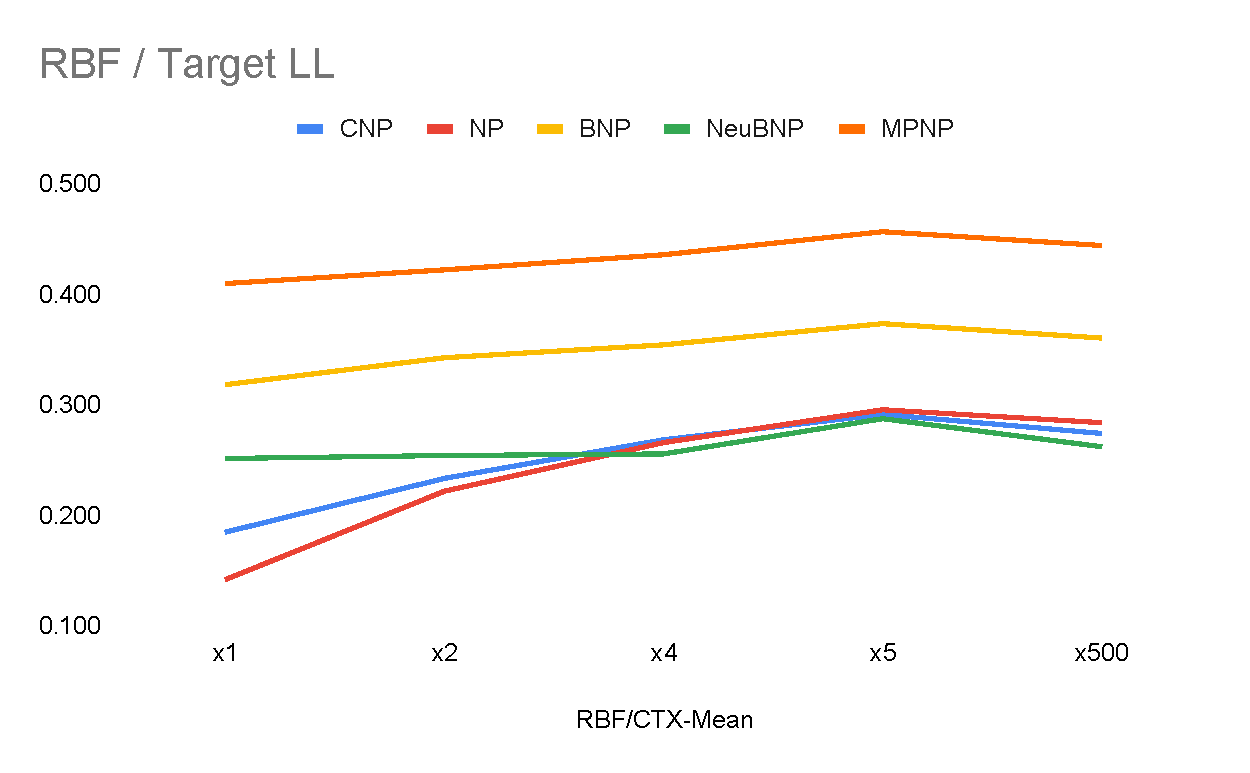
\includegraphics[width=0.24\textwidth]{figure/gp_finite/rbf_tar_cnps.pdf}
%     % 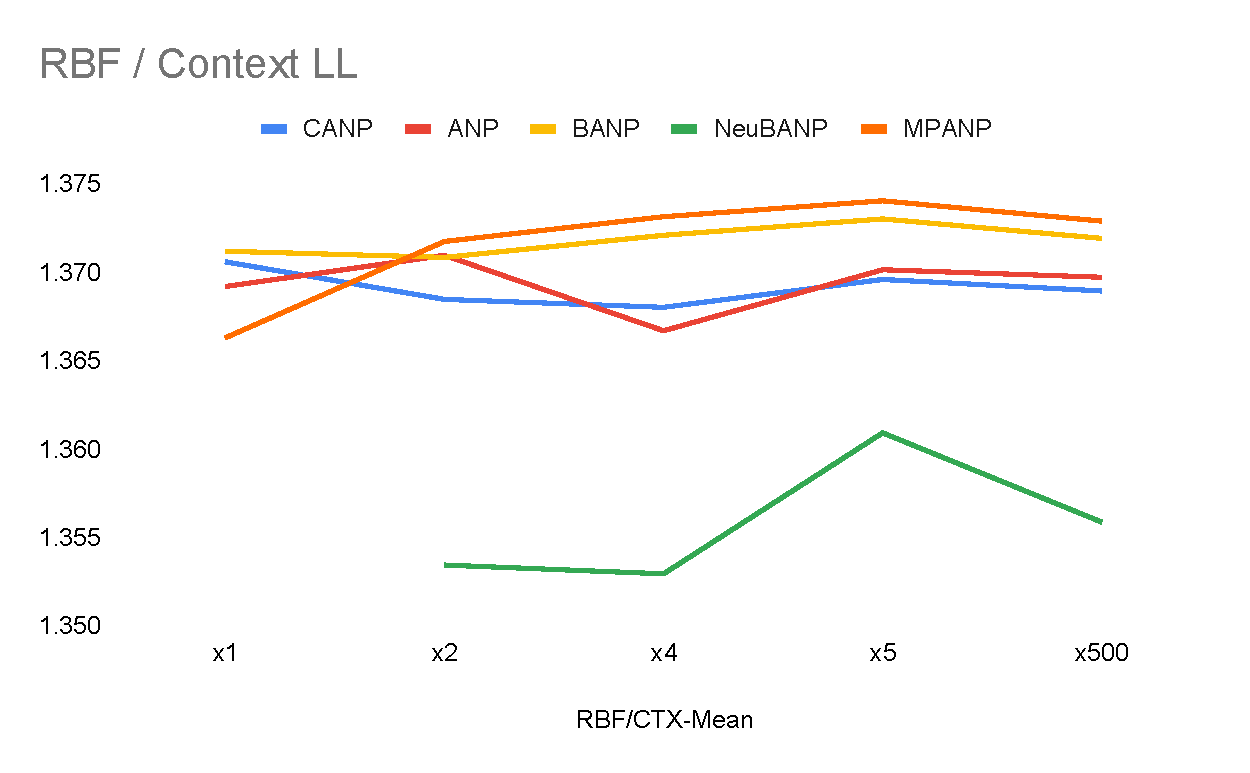
\includegraphics[width=0.24\textwidth]{figure/gp_finite/rbf_ctx_canps.pdf}
%     % 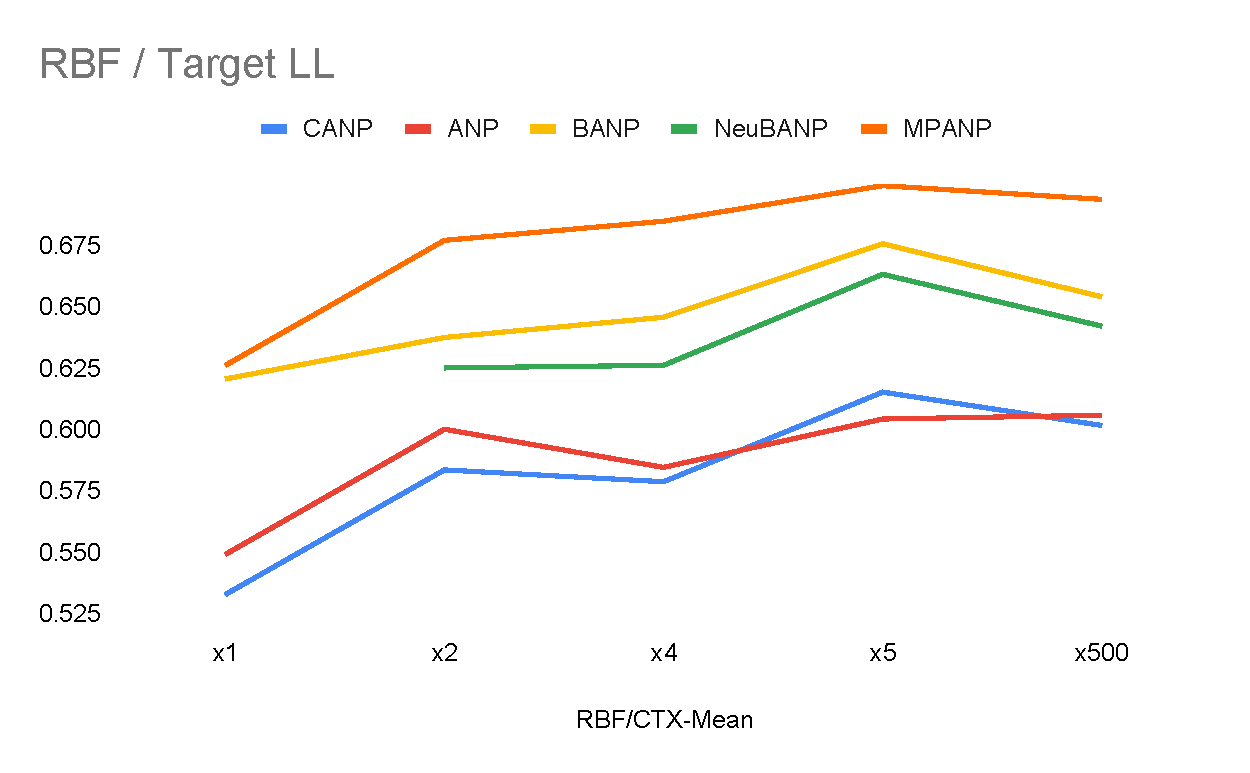
\includegraphics[width=0.24\textwidth]{figure/gp_finite/rbf_tar_canps.pdf}
%     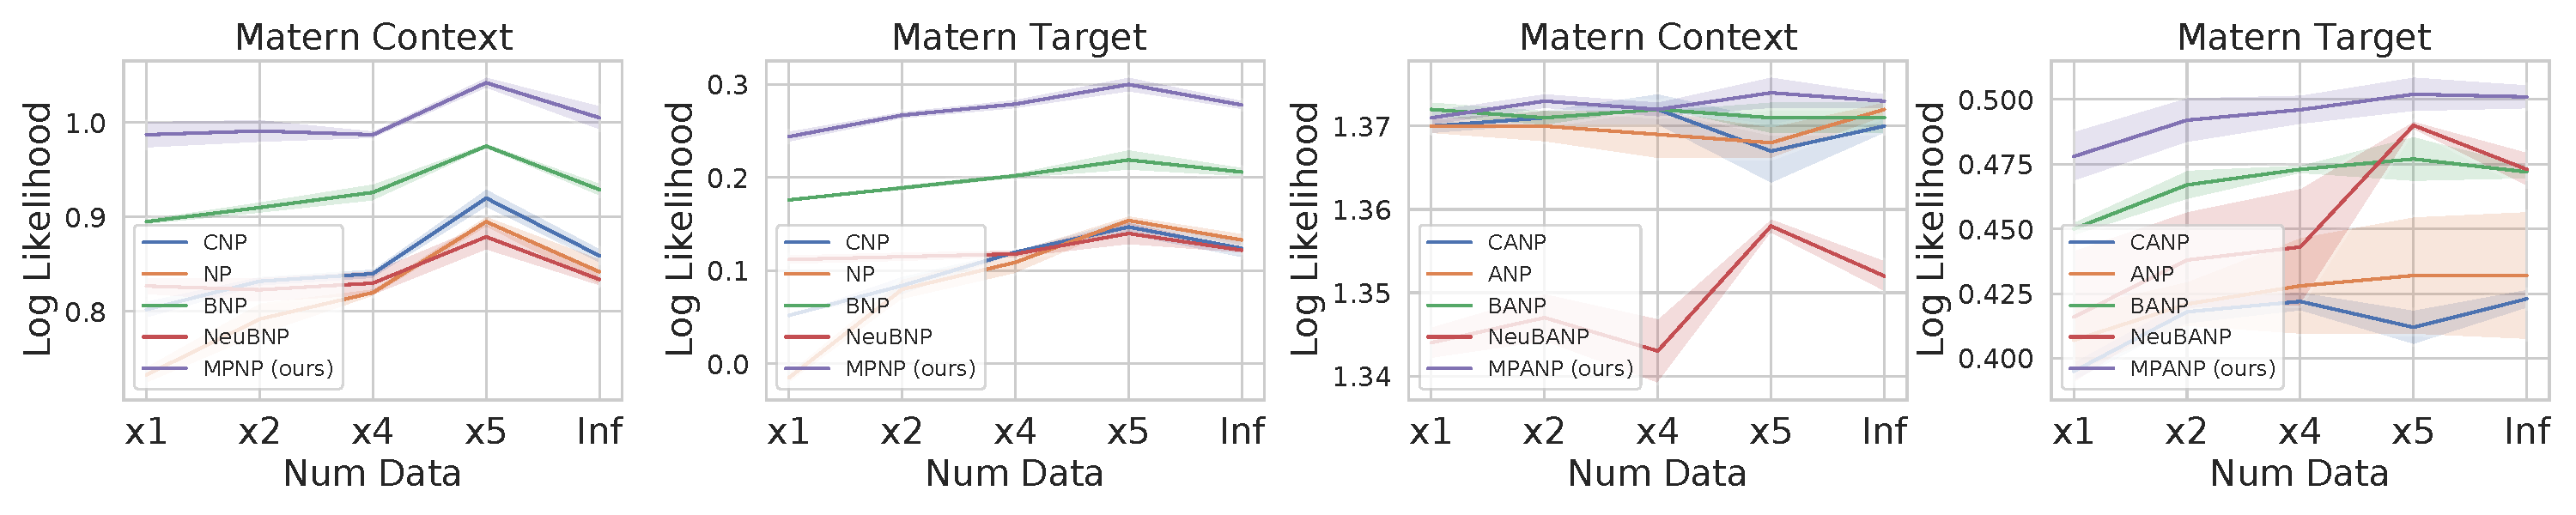
\includegraphics[width=\textwidth]{figure/out_matern.pdf}
%     \caption{Results of Finite Training Dataset experiments with Matern 5/2 kernel.}
%     \label{fig:figure_gp_finite_matern}
% \end{figure}
% \begin{figure}[t]
%     \centering
%     % 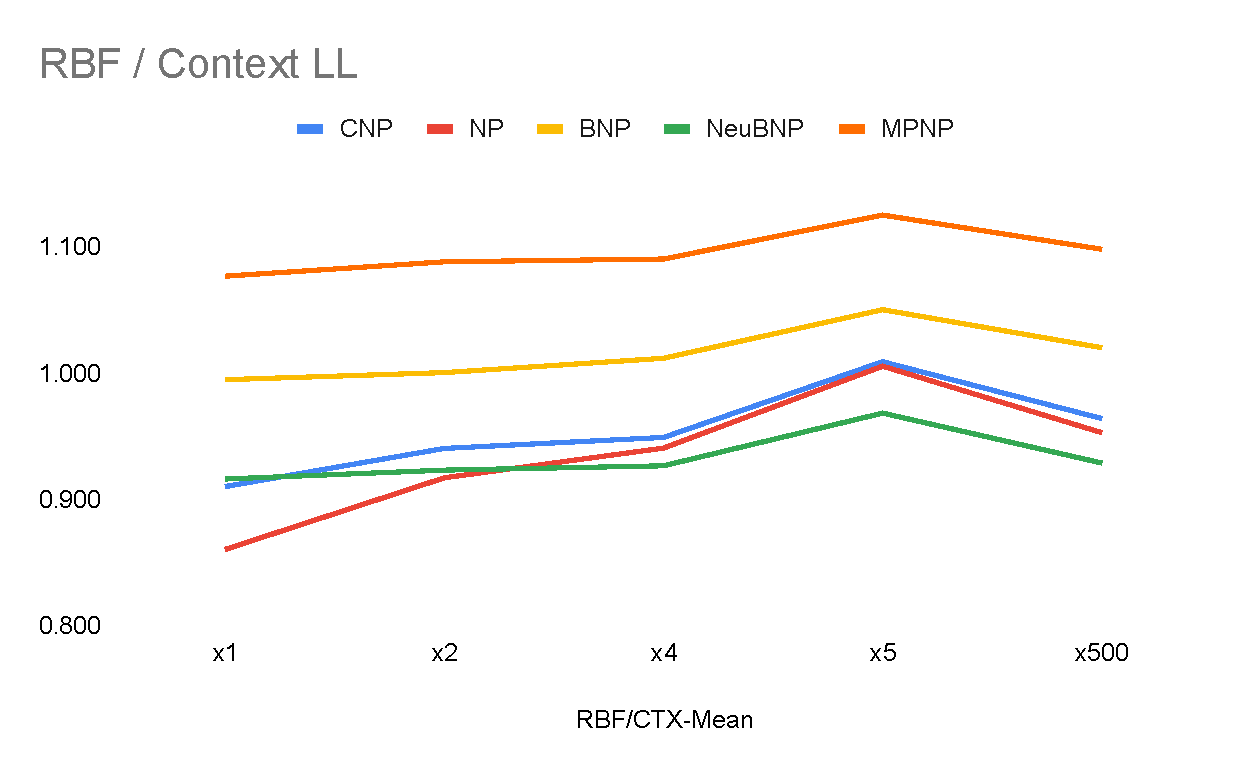
\includegraphics[width=0.24\textwidth]{figure/gp_finite/rbf_ctx_cnps.pdf}
%     % 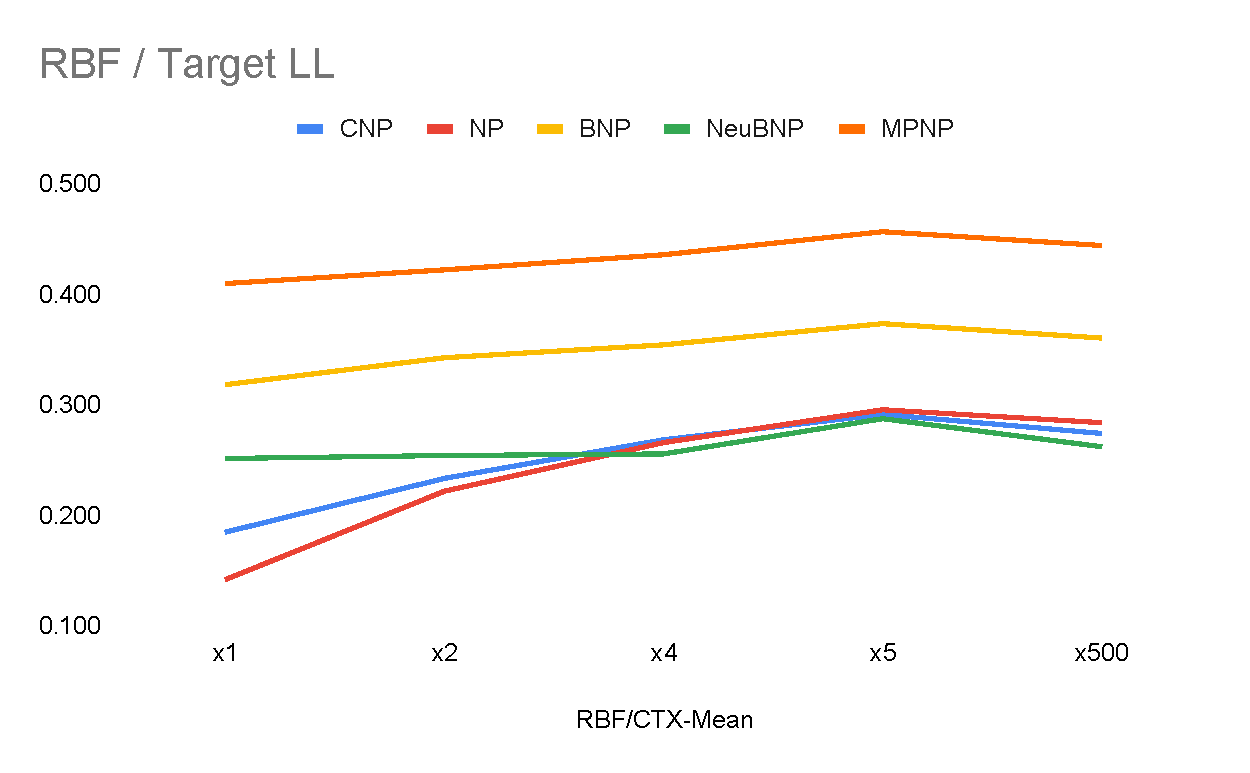
\includegraphics[width=0.24\textwidth]{figure/gp_finite/rbf_tar_cnps.pdf}
%     % 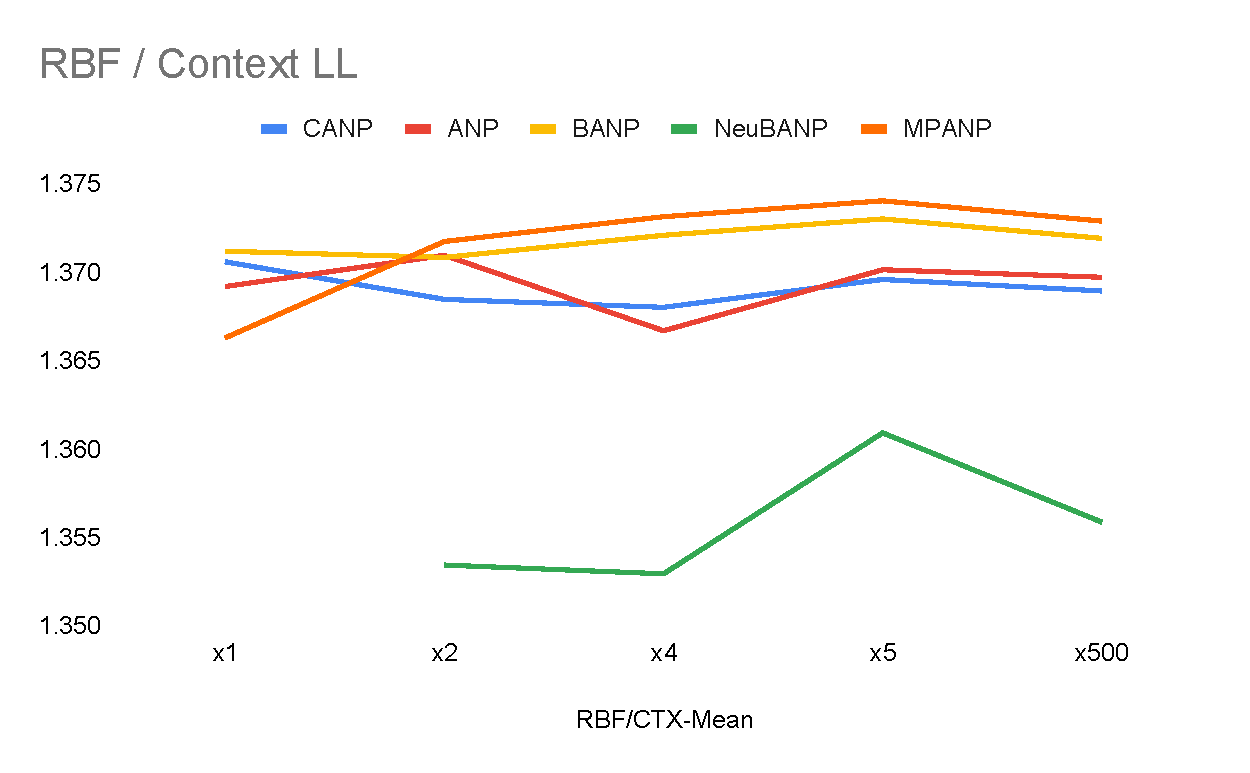
\includegraphics[width=0.24\textwidth]{figure/gp_finite/rbf_ctx_canps.pdf}
%     % 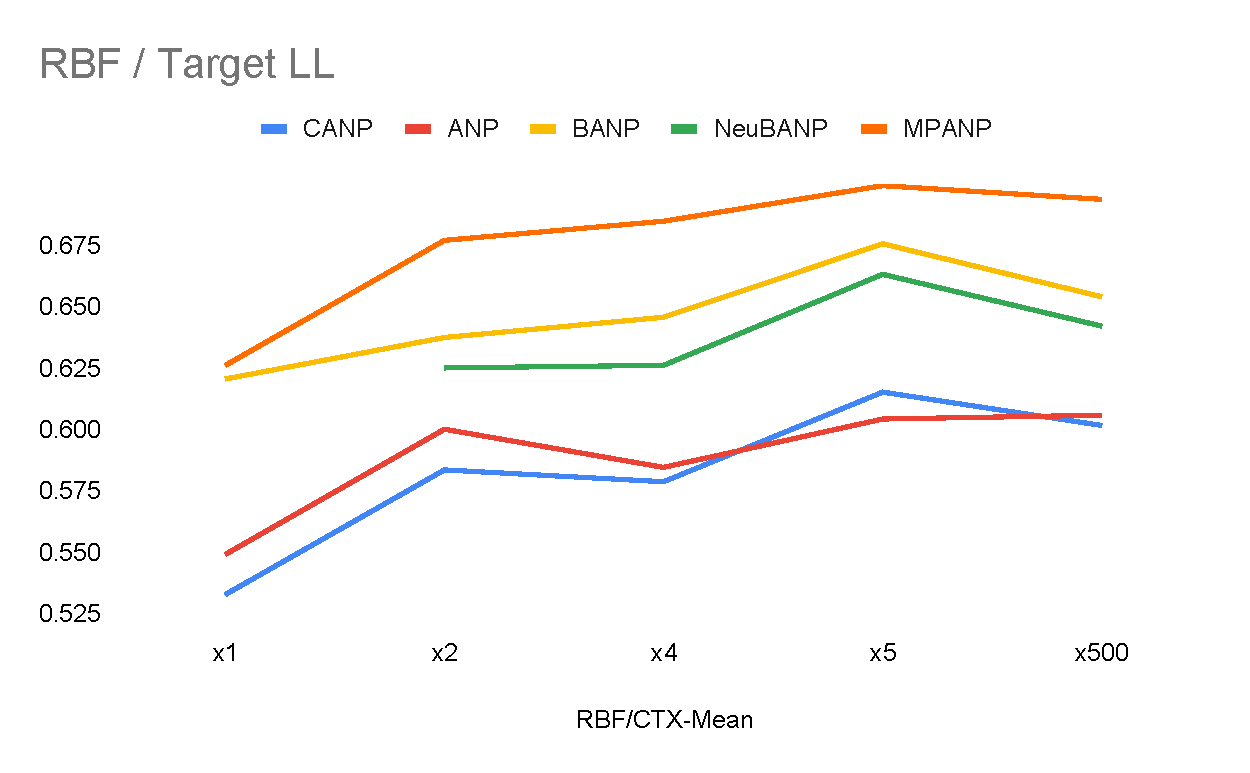
\includegraphics[width=0.24\textwidth]{figure/gp_finite/rbf_tar_canps.pdf}
%     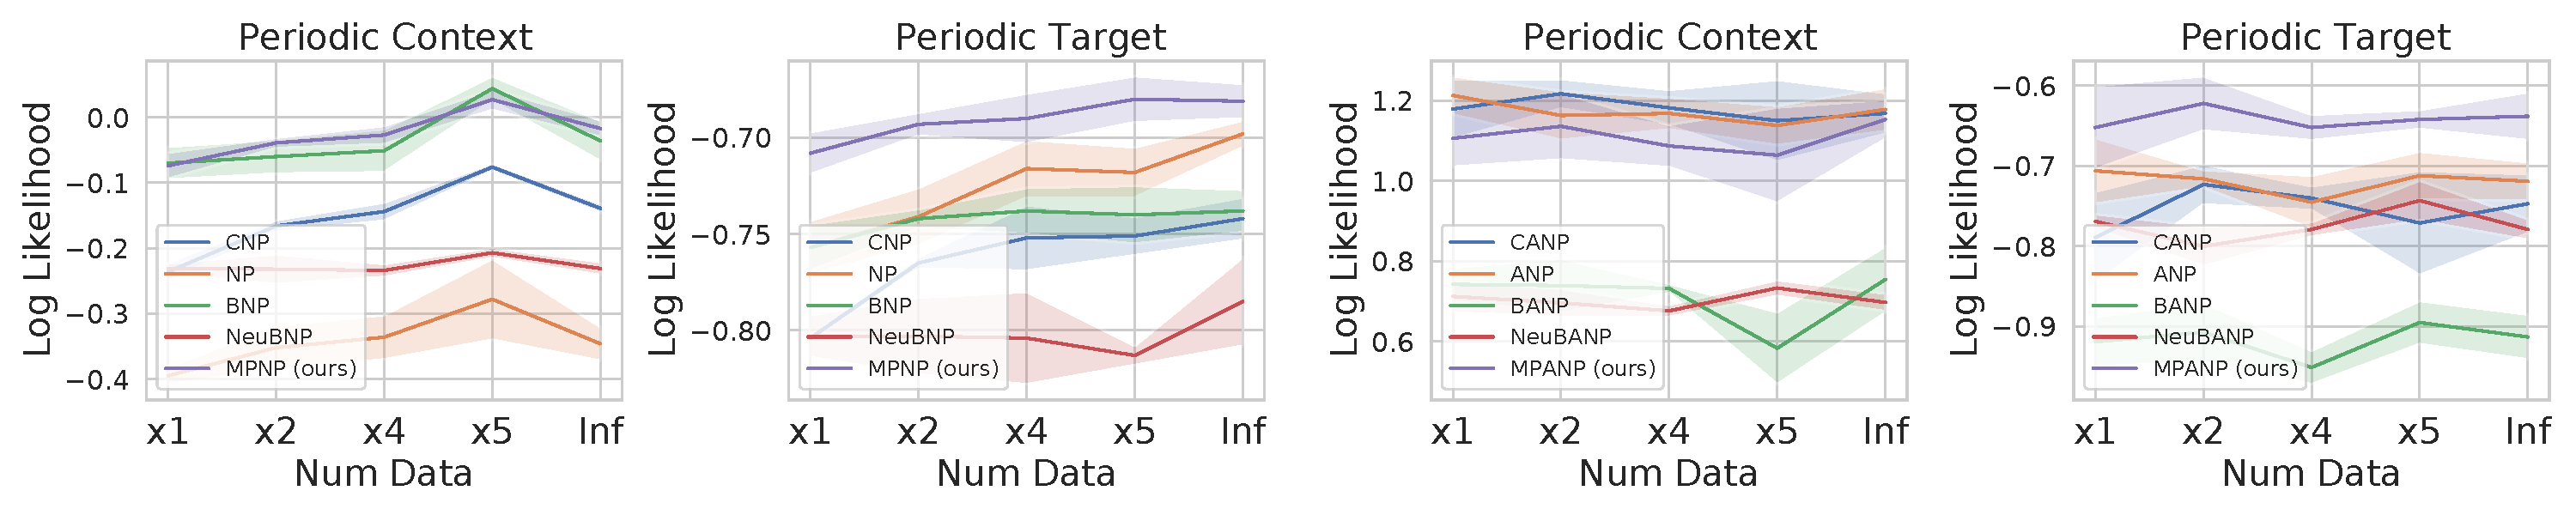
\includegraphics[width=\textwidth]{figure/out_periodic.pdf}
%     \caption{Results of Finite Training Dataset experiments with Periodic kernel.}
%     \label{fig:figure_gp_finite_periodic}
% \end{figure}
% \begin{figure}[t]
%     \centering
%     % 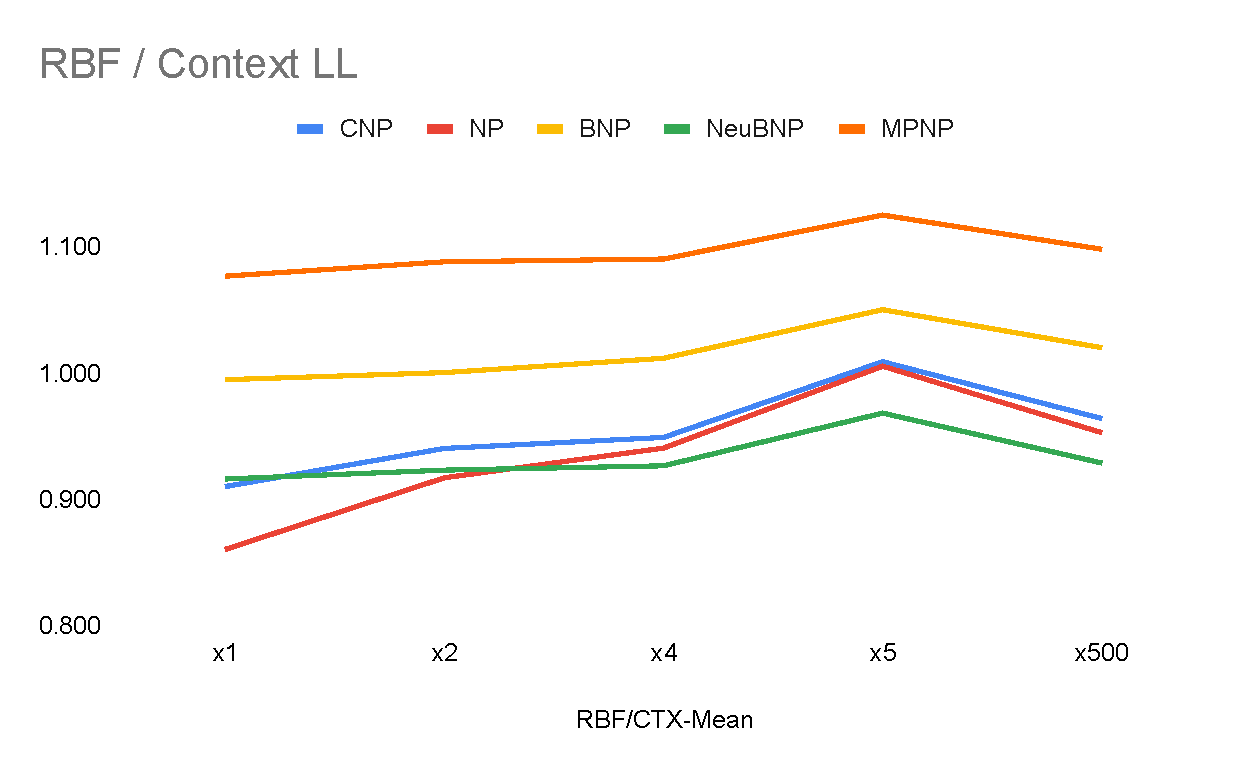
\includegraphics[width=0.24\textwidth]{figure/gp_finite/rbf_ctx_cnps.pdf}
%     % 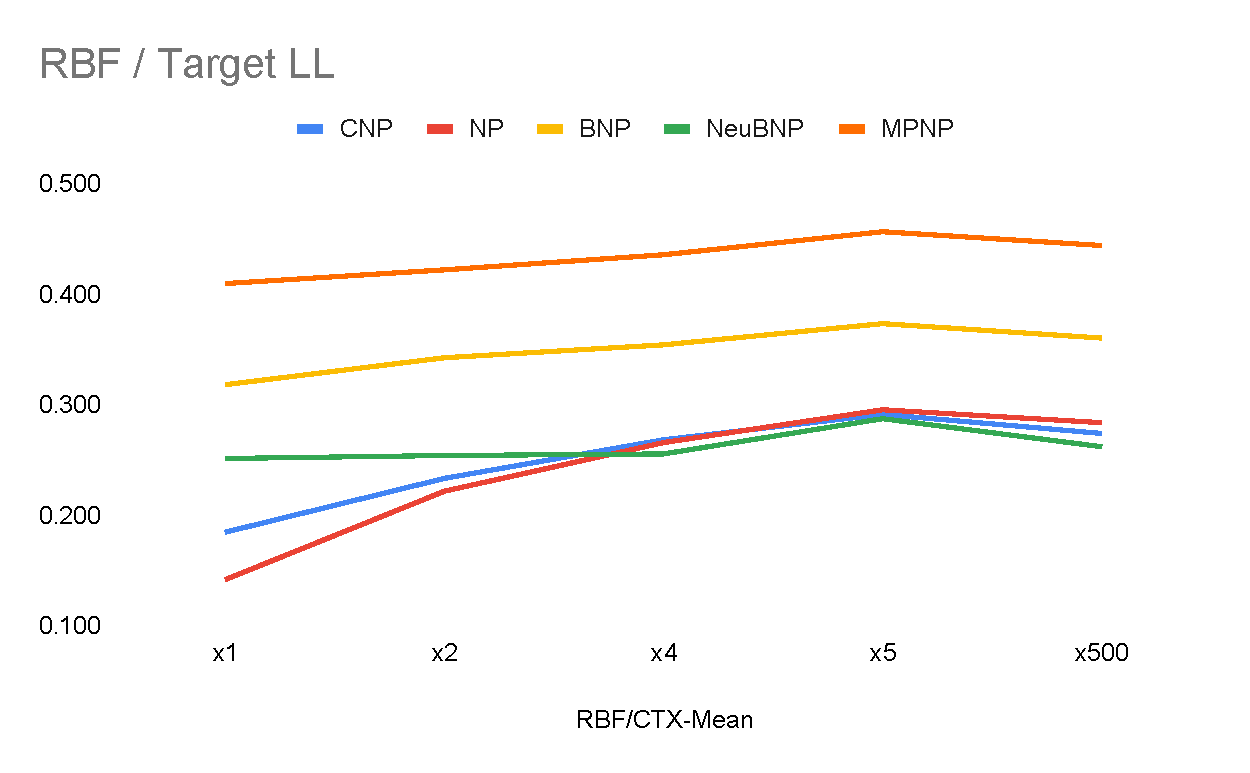
\includegraphics[width=0.24\textwidth]{figure/gp_finite/rbf_tar_cnps.pdf}
%     % 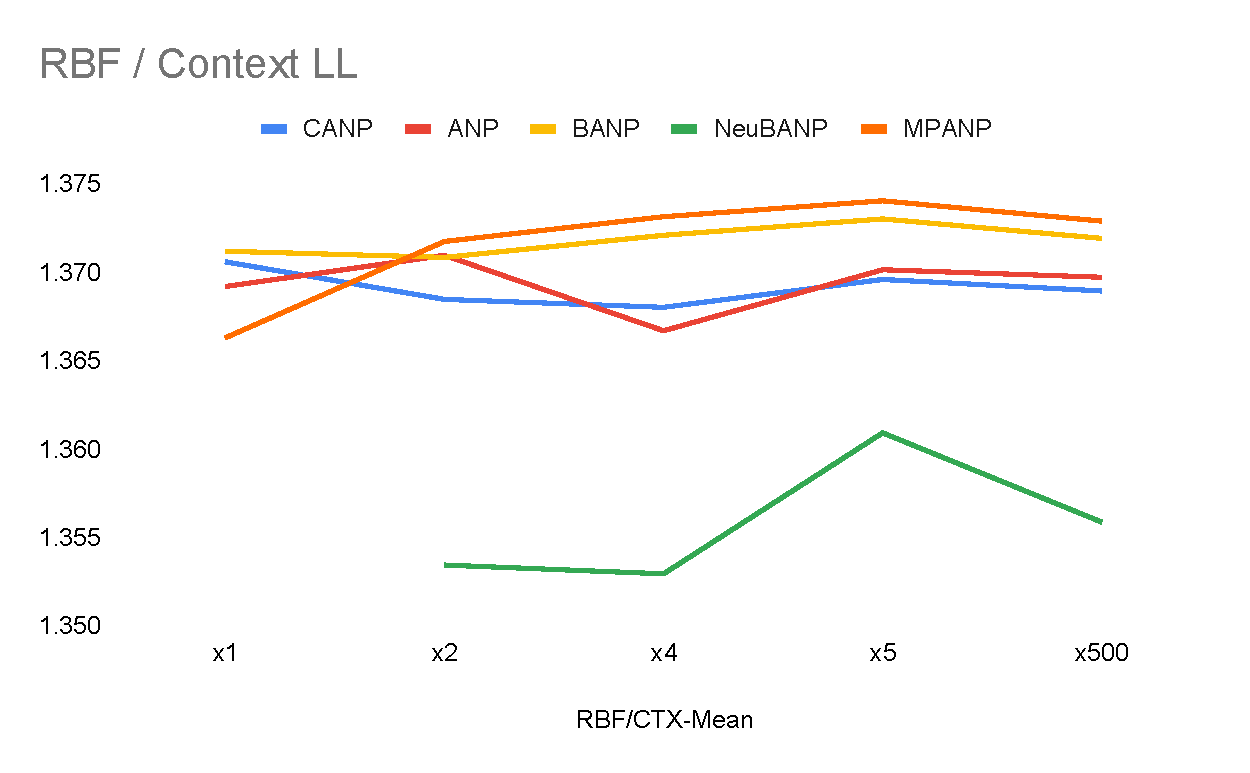
\includegraphics[width=0.24\textwidth]{figure/gp_finite/rbf_ctx_canps.pdf}
%     % 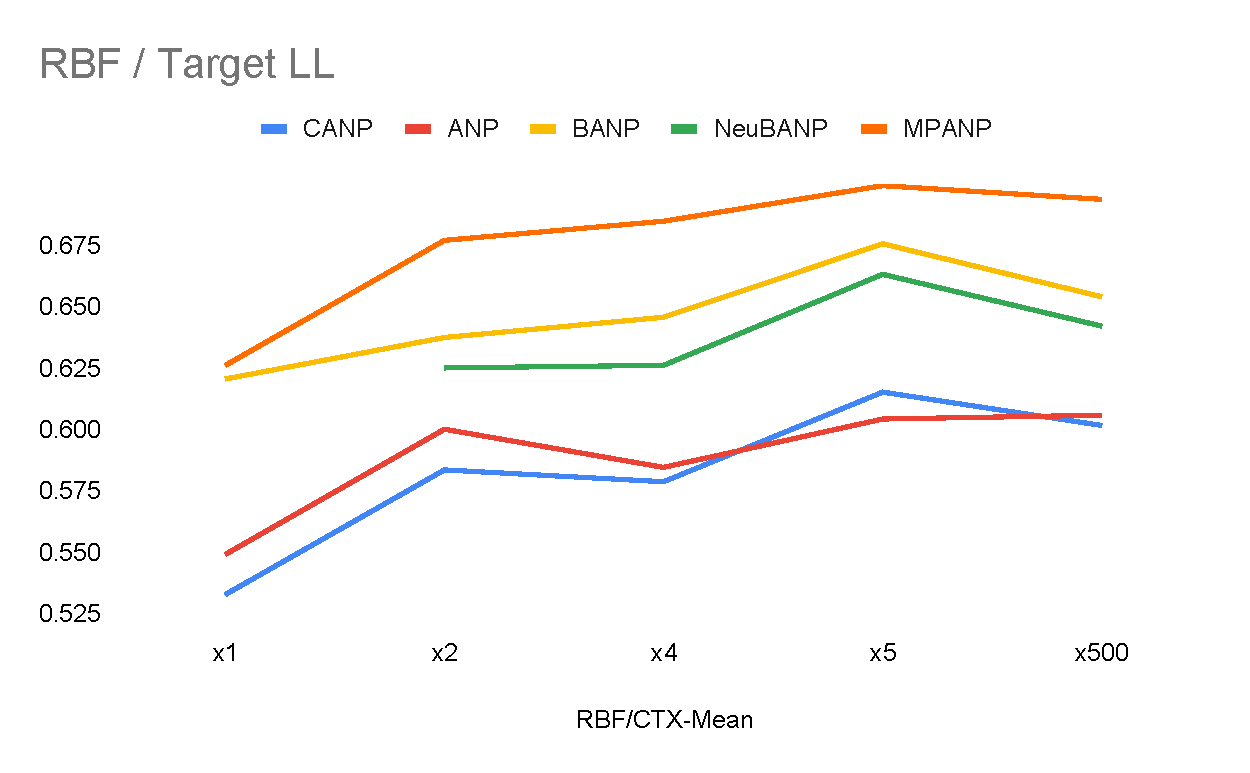
\includegraphics[width=0.24\textwidth]{figure/gp_finite/rbf_tar_canps.pdf}
%     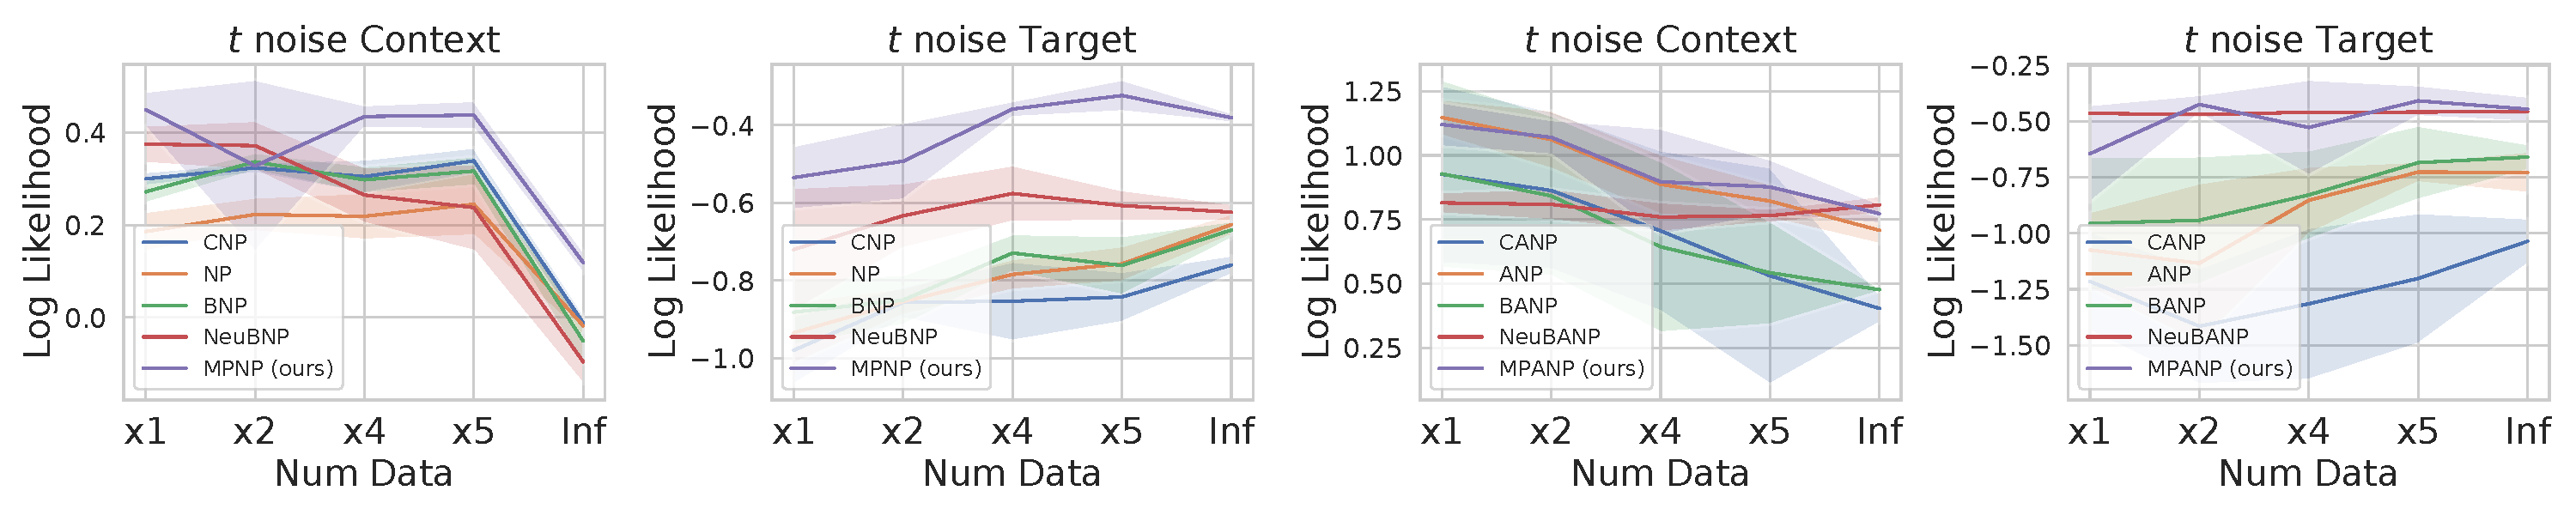
\includegraphics[width=\textwidth]{figure/out_t_noise.pdf}
%     \caption{Results of Finite Training Dataset experiments with RBF kernel with Students' $t$ distributed noise.}
%     \label{fig:figure_gp_finite_t_noise}
% \end{figure}
% In this section, we presents the remain results of Finite Training Dataset in \cref{main:subsec:infinite_training} for the kernels other than RBF.
% Here as you can see in \cref{fig:figure_gp_finite_matern}, \cref{fig:figure_gp_finite_periodic} and \cref{fig:figure_gp_finite_t_noise}, \glspl{mpnp} consistently outperforms the baselines.

% \subsection{Predator-Prey Model}
% \label{app:subsec:predator-prey}
% \begin{table}[t]
    \caption{Context and target log likelihood values on Lotka Volterra simulated data and real data. Performances are measured over 4 seeds.\\}
    \label{tab:table_lotka}
    \centering
    \scriptsize
    \renewcommand{\arraystretch}{0.9}
    \resizebox{0.6\textwidth}{!}{
    \begin{tabular}{lrrrr}
        \toprule
        \multirow{3}{*}{Model} & \multicolumn{2}{r}{Simulation}                            & \multicolumn{2}{r}{Real}                                    \\
                                 \cmidrule(lr){2-3}                                          \cmidrule(lr){4-5}                                       
                               & context                     & target                      & context                     & target                        \\
        \midrule
        CNP                    &         0.161  $\pm{0.038}$ &        -0.192  $\pm{0.032}$ &         -2.759  $\pm{0.027}$ &         -3.278  $\pm{0.041}$ \\
        NP                     &         0.185  $\pm{0.036}$ &        -0.152  $\pm{0.037}$ &         -2.707  $\pm{0.027}$ &         -3.200  $\pm{0.042}$ \\
        BNP                    &         0.402  $\pm{0.009}$ &         0.038  $\pm{0.018}$ &         -2.723  $\pm{0.032}$ &         -3.168  $\pm{0.041}$ \\
        NeuBNP                 &         0.114  $\pm{0.059}$ &        -0.267  $\pm{0.053}$ &         -2.794  $\pm{0.073}$ &         -3.128  $\pm{0.045}$ \\
        MPNP (ours)            & \textBF{0.403} $\pm{0.047}$ & \textBF{0.116} $\pm{0.035}$ & \textBF{-2.648} $\pm{0.041}$ & \textBF{-3.106} $\pm{0.021}$ \\
        \cmidrule(lr){1-1}       \cmidrule(lr){2-3}                                          \cmidrule(lr){4-5}                                       
        CANP                   &         2.498  $\pm{0.018}$ &         1.541  $\pm{0.010}$ &          1.836  $\pm{0.169}$ &         -6.873  $\pm{0.612}$ \\
        ANP                    &         2.528  $\pm{0.026}$ &         1.643  $\pm{0.011}$ & \textBF{ 2.058} $\pm{0.080}$ &         -5.454  $\pm{0.408}$ \\
        BANP                   & \textBF{2.605} $\pm{0.021}$ &         1.685  $\pm{0.032}$ &          2.054  $\pm{0.126}$ & \textBF{-3.388} $\pm{0.446}$ \\
        NeuBANP                &         2.421  $\pm{0.024}$ &         1.358  $\pm{0.026}$ &          1.878  $\pm{0.050}$ &         -3.739  $\pm{0.240}$ \\
        MPANP (ours)           &         2.554  $\pm{0.025}$ & \textBF{1.769} $\pm{0.013}$ &          1.946  $\pm{0.136}$ &         -4.942  $\pm{0.387}$ \\
        \bottomrule
    \end{tabular}}
\end{table}
% Following \citet{lee2020bootstrapping}, we conducted the predator-prey population regression experiments.
% We first trained the models using the simulation datasets which are generated from a Lotka-Volterra model~\citep{wilkinson2018stochastic} with the simulation settings followed by \citet{lee2020bootstrapping}. Then tested on the generated simulation test dataset and real-world dataset which is called Hudson's Bay hare-lynx data.
% As mentioned in \citet{lee2020bootstrapping}, the real-world dataset shows different tendency from generated simulation datasets, so we can also treat this experiment as model-data mismatch experiments.
% In \cref{tab:table_lotka}, we can see that \glspl{mpnp} outperforms the other baselines for the test simulation datasets but underperforms in the real-world dataset compare to other baselines especially in the \gls{mpanp} case.
% This also shows that model-data mismatch is an open problem for the \glspl{mpnp}. 

%%%%%%%%%%%%%%%%%%%%%%%%%%%%%%%%%%%%%%%%%%%%%%%%%%
\section{Experimental Details}
\label{app:sec:details}
%%%%%%%%%%%%%%%%%%%%%%%%%%%%%%%%%%%%%%%%%%%%%%%%%%
We attached our code in supplementary material. Our codes used python libraries JAX~\citep{jax2018github}, Flax~\citep{flax2020github} and Optax~\citep{optax2020github}. 
These python libraries are available under the Apache-2.0 license\footnote{\href{https://www.apache.org/licenses/LICENSE-2.0}{https://www.apache.org/licenses/LICENSE-2.0}}.


We conducted all experiments on a single NVIDIA GeForce RTX 3090 GPU, except for the image completion tasks presented in~\cref{main:sec:experiments:imagecompletion}; we used 8 TPUv3 cores supported by TPU Research Cloud\footnote{\href{https://sites.research.google/trc/about/}{https://sites.research.google/trc/about/}} for the 2D image completion task. For optimization, we used Adam~\citep{kingma2015adam} optimizer with a cosine learning rate schedule. Unless specified, we selected the base learning rate from a grid of $\{5 \times 10^{-4.50}, 5 \times 10^{-4.25}, 5 \times 10^{-4.00}, 5 \times 10^{-3.75}, 5 \times 10^{-3.50}\}$ based on validation task log-likelihood.


% For all experiments, we use Adam optimizer with learning rate $5 \cdot 10^{-4}$. For image completion tasks, we also use cosine learning rate scheduling.

%%%%%%%%%%%%%%%%%%%%%%%%%%%%%%%%%%%%%%%%%%%%%%%%%%
% \subsection{Experimental Resources}
% We conduct most of the experiments on 8 TPUv3 cores, supported by TPU Research Cloud\footnote{\href{https://sites.research.google/trc/about/}{https://sites.research.google/trc/about/}} and the others on 8 RTX3090 cores.

%%%%%%%%%%%%%%%%%%%%%%%%%%%%%%%%%%%%%%%%%%%%%%%%%%
\subsection{Evaluation metric}
Following \citet{le2018empirical},  for \gls{cnp} and \gls{canp}, which are deterministic models, we used the normalized predictive log-likelihood $\frac{1}{n}\sum_{i=1}^n\log p(y_i|x_i,Z_c)$. For other models, we used a approximation of the normalized predictive log-likelihood as:
\[
\frac{1}{n}\sum_{i=1}^n\log p(y_i|x_i,Z_c)\approx \frac{1}{n}\sum_{i=1}^n\log\frac{1}{K}\sum_{k=1}^K p(y_i|x_i,\theta^{(k)}),
\]
where $\theta^{k}$s are independent samples for $k\in[K]$.
\subsection{1D Regression}
To generate tasks $(Z, c)$, we first sample $x \iidsim \text{Unif}(-2, 2)$ and generate $Y$ using each kernel. We use RBF kernel $k(x, x') = s^2 \cdot \exp\left(\frac{-|| x - x' ||^2}{2\ell^2}\right)$, Matern $5/2$ kernel $k(x, x') = s^2 \cdot \left( 1 + \frac{\sqrt{5}d}{\ell} + \frac{5d^2}{3\ell^2} \right)$, and periodic kernel $k(x, x') = s^2 \cdot \exp\left( \frac{-2 \sin^2 (\pi||x-x'||^2 / p)}{\ell^2} \right)$ where all kernels use $s \sim \text{Unif}(0.1. 1.0)$, $\ell \sim \text{Unif}(0.1. 0.6)$, and $p \sim \text{Unif}(0.1. 0.5)$. To generate t-noise dataset, we use Student-$t$ with degree of freedom $2.1$ to sample noise $\epsilon \sim \gamma \cdot \calT(2.1)$ where $\gamma \sim \text{Unif}(0, 0.15)$. Then we add the noise to the curves generated from RBF kernel. We draw index set $|c| \sim \text{Unif}(3, 50 - 3)$ and $n - |c| \sim \text{Unif}(3, 50 - |c|)$ to maintain $\max |Z| \leq 50$. We use a batch size of $256$ for training.

%%%%%%%%%%%%%%%%%%%%%%%%%%%%%%%%%%%%%%%%%%%%%%%%%%
\subsection{Image Completion}

We use the following datasets for image completion experiments.

\paragraph{MNIST}
We split MNIST~\citep{lecun1998gradient} train dataset into train set with 50,000 samples and validation set with 10,000 samples. We use whole 10,000 samples in test dataset as test set. We make $28 \times 28$ grids which both axes starting from $-0.5$ to $0.5$ to indicate the coordinate of pixels, and normalize pixel values into $[-0.5, 0.5]$. We use a batch size of $128$ for training.

\paragraph{SVHN}
We split SVHN~\citep{netzer2011reading} train dataset into train set with 58,600 samples and validation set with 14,657 samples. We use whole 26,032 samples in test dataset as test set. We make $32 \times 32$ grids which both axes starting from $-0.5$ to $0.5$ to indicate the coordinate of pixels, and normalize pixel values into $[-0.5, 0.5]$. We use a batch size of $128$ for training.

\paragraph{CelebA}
We use splits of CelebA~\citep{liu2015faceattributes} dataset as provided (162,770 train samples, 19,867 validation samples, 19,962 test samples). We crop $32 \times 32$ pixels of center of images. We make $32 \times 32$ grids which both axes starting from $-0.5$ to $0.5$ to indicate the coordinate of pixels, and normalize pixel values into $[-0.5, 0.5]$. We use a batch size of $128$ for training.

%%%%%%%%%%%%%%%%%%%%%%%%%%%%%%%%%%%%%%%%%%%%%%%%%%

\subsection{Bayesian Optimization}
\label{app:sec:details:bo}

We use the following benchmark functions for Bayesian optimization experiments. Throughout the experiments, we adjust the function to  have the domain of $[-2.0, 2.0]$.
\paragraph{\citet{gramacy2012cases} function}
\[
f(x)=\frac{\sin(10\pi x)}{2x} + (x-1)^4,
\]
where $x\in [0.5,2.5]$ and a global optimum is at $x^\ast\approx 0.5486$.
\paragraph{\citet{sobester2008engineering} function}
\[
f(x)=(6x-2)^2\sin (12x-4),
\]
where $x\in [0,1]$ and a global optimum is at $x^\ast\approx0.7572$.


% \section{Ablation Study}
% \label{app:sec:ablation_study}
% \begin{table}[t]
%     \caption{Context and target log likelihood values on data sampled from Gaussian Processes with various kernel. Here we trained the same model with different losses. Performances are measured over 4 seeds.\\}
%     \label{tab:table_gp_inf_ablation}
%     \centering
%     \scriptsize
%     \renewcommand{\arraystretch}{0.9}
%     \resizebox{0.95\textwidth}{!}{
%     \begin{tabular}{lrrrrrrrrrrrr}
%         \toprule
%         \multirow{3}{*}{Model} & \multicolumn{2}{r}{RBF}                                   & \multicolumn{2}{r}{Matern}                                & \multicolumn{2}{r}{Periodic}                                & \multicolumn{2}{r}{$t$-noise}                               \\
%                                  \cmidrule(lr){2-3}                                          \cmidrule(lr){4-5}                                          \cmidrule(lr){6-7}                                            \cmidrule(lr){8-9}
%                               & context                     & target                      & context                     & target                      & context                      & target                       & context                      & target                       \\
%         \midrule
% MPNP (ours)                                              &         1.086  $\pm{0.005}$ &         0.457  $\pm{0.002}$ &         1.005  $\pm{0.014}$ &         0.278  $\pm{0.006}$ &         -0.017  $\pm{0.013}$ &         -0.681  $\pm{0.009}$ &          0.119  $\pm{0.025}$ &         -0.381  $\pm{0.013}$ \\
% - $\calL_{\text{amort}}$                                 &         1.146  $\pm{0.010}$ &         0.487  $\pm{0.009}$ &         1.064  $\pm{0.002}$ &         0.300  $\pm{0.005}$ &         -0.002  $\pm{0.039}$ &         -0.673  $\pm{0.011}$ &          0.166  $\pm{0.027}$ &         -0.372  $\pm{0.043}$ \\
% - $\calL_{\text{pseudo}}$                                &         1.090  $\pm{0.008}$ &         0.445  $\pm{0.006}$ &         1.012  $\pm{0.004}$ &         0.277  $\pm{0.007}$ &          0.058  $\pm{0.018}$ &         -0.669  $\pm{0.007}$ &          0.239  $\pm{0.006}$ &         -0.348  $\pm{0.023}$ \\
% - $\calL_{\text{amort}}$ - $\calL_{\text{pseudo}}$       &         1.160  $\pm{0.008}$ &         0.493  $\pm{0.006}$ &         1.092  $\pm{0.012}$ &         0.320  $\pm{0.004}$ &          0.074  $\pm{0.019}$ &         -0.666  $\pm{0.010}$ &          0.365  $\pm{0.010}$ &         -0.416  $\pm{0.086}$ \\
% \cmidrule(lr){1-1}       \cmidrule(lr){2-3}                                          \cmidrule(lr){4-5}                                          \cmidrule(lr){6-7}                                            \cmidrule(lr){8-9}
% MPANP (ours)                                             &         1.374  $\pm{0.000}$ &         0.698  $\pm{0.007}$ &         1.373  $\pm{0.001}$ &         0.501  $\pm{0.005}$ &          1.153  $\pm{0.049}$ &         -0.638  $\pm{0.030}$ &          0.773  $\pm{0.039}$ &         -0.446  $\pm{0.057}$ \\
% - $\calL_{\text{amort}}$                                 &         1.359  $\pm{0.001}$ &         0.703  $\pm{0.001}$ &         1.351  $\pm{0.006}$ &         0.501  $\pm{0.004}$ &          1.007  $\pm{0.064}$ &         -0.651  $\pm{0.032}$ &          0.496  $\pm{0.023}$ &         -0.520  $\pm{0.059}$ \\
% - $\calL_{\text{pseudo}}$                                &         1.375  $\pm{0.000}$ &         0.678  $\pm{0.010}$ &         1.373  $\pm{0.002}$ &         0.480  $\pm{0.007}$ &          1.129  $\pm{0.065}$ &         -0.606  $\pm{0.005}$ &          0.786  $\pm{0.056}$ &         -0.433  $\pm{0.011}$ \\
% - $\calL_{\text{amort}}$ - $\calL_{\text{pseudo}}$       &         1.374  $\pm{0.001}$ &         0.680  $\pm{0.002}$ &         1.370  $\pm{0.007}$ &         0.486  $\pm{0.014}$ &          0.811  $\pm{0.142}$ &         -0.789  $\pm{0.132}$ &          0.826  $\pm{0.030}$ &         -0.428  $\pm{0.037}$ \\
%         \bottomrule
%     \end{tabular}}
% \end{table}

% \begin{figure}[t]
%     \centering
%     \includegraphics[width = 0.32\textwidth]{figure/sample plot 9 amort.pdf}
%     \includegraphics[width = 0.32\textwidth]{figure/sample plot 9 pseudo.pdf}
%     \includegraphics[width = 0.32\textwidth]{figure/sample plot 9 both.pdf}
%     % \includegraphics[width = 0.32\textwidth]{figure/data plot 9.pdf}
%     % \includegraphics[width = 0.32\textwidth]{figure/sample plot 9.pdf}
%     % \includegraphics[width = 0.32\textwidth]{figure/posterior plot 9.pdf}
%     \caption{Generated pseudo context data samples of MPANP in 1d regression task. (Left) Generated pseudo context when we remove the term $\calL_{\text{amort}}$ from the loss $\calL$. (Middle) Generated pseudo context when we remove the term $\calL_{\text{pseudo}}$ from the loss $\calL$. (Right) Generated pseudo context when we remove the terms $\calL_{\text{amort}}$ and $\calL_{\text{pseudo}}$ from the loss $\calL$.} 
%     \label{fig:feature_ablation}
% \end{figure}

% In this section, we conduct some ablation studies on loss function and report the generated pseudo context data and the performances of the \glspl{mpnp} in 1D regression.
% As our loss function essentially contain the $\calL_{\text{marg}}$ term, we conduct the ablation studies on the other terms ($\calL_{\text{pseudo}}$ and $\calL_{\text{amort}}$). 
% We have three cases i) loss function $\calL$ without $\calL_{\text{amort}}$, ii) loss function $\calL$ without $\calL_{\text{pseudo}}$ and iii) loss function $\calL$ without $\calL_{\text{amort}}$ and $\calL_{\text{pseudo}}$.
% We report the performances of the three cases in \cref{tab:table_gp_inf_ablation}.
% Also we present the generated pseudo context data from the three cases in \cref{fig:feature_ablation}.
% Here you can see that without any term in $\calL$, the model cannot actually generate meaningful pseudo context dataset from real context dataset.
\section{Directly Generating Input Model}
\label{app:sec:directly_generating_input}
In this section, we present our model generating pseudo contexts directly in the input space.
We will present two kinds of model structure, i) directly generating pseudo context pair $(x,y)$ simultaneously by ISAB, ii) generating pseudo context data $x$ and $y$, sequentially. 
\subsection{Construction}
\paragraph{Generating pseudo context pair simultaneously.}
The generator of our first model which simultaneously generating pseudo context pair $(x',y')$, takes real context dataset $Z_c$ as input and outputs pseudo context dataset $Z'$. 
Here the generator is the one layer ISAB module.
Then we concatenate $Z_c$ and $Z'$ in order to treat this concatenated set as context dataset.
Then the encoder takes this concatenated context set as input.
And the others are the same with \gls{cnp} or \gls{canp}.
\paragraph{Sequentially generating pseudo context data \texorpdfstring{$x$}{x} and \texorpdfstring{$y$}{y}}
In this model, the generator takes real context dataset $Z_c$ as input and outputs only $x'$s of $Z'$. 
Here the generator is the one layer ISAB module with additional one linear layer.
Then we consider these $x'$s as our target dataset and find the mean and variance of $y'$ for each $x'$ by forwarding the model with context dataset $Z_c$ and target $x'$.
We sample $y'$ from the Gaussian distribution with mean and variance from the prior step.
We again concatenate $Z_c$ with $Z'$ and use them as context dataset.

\paragraph{Training}
Having directly generated a pseudo context set, we construct our empirical density as
\[
g_N(z) = \frac{1}{N}\bigg(\sum_{i\in c}\delta_{z_i}(z) + \sum_{i=1}^{N-|c|} \delta_{z'_i}(z)\bigg).
\]
Given $g_N$, we find the function parameter $\theta$ as
\[
\theta(g_N) := \argmin_\theta \int \ell(z, \theta) g_N(dz),
\]
where we simply choose $l(z,\theta):=-\log \calN (y|\mu_\theta(x),\sigma_\theta^2(x)I_{d_{out}})$.
In order to train the directly generating input model, which well approximate $\theta(g_N)$, we should construct different objective function from \cref{eq:mpnp_term_whole} because we can compute the exact $\int \ell(z, \theta) g_N(dz)$, unlike the feature generating model.
First, we approximate the marginal likelihood which is,
\[
\label{eq:direct1}
\log p(Y|X, Z_c) \approx \log \Bigg[ \frac{1}{K} \sum_{k=1}^K \exp\bigg(-\sum_{i\in [n]}\ell(z_i, \tilde\theta(Z_c\cup Z'^{(k)}))\bigg)
\Bigg] := -\calL_\text{marg}(\tau,\phi),
\]
where $Z'^{(1)},\dots, Z'^{(K)}\iidsim p(Z'|Z_c;\phi_\text{pred})$.
\cref{eq:direct1} is the same training object with \cref{eq:mpnp_term1}.
As we mentioned in \cref{main:subsec:training}, if we are given sufficiently well approximated $\Tilde{\theta}(Z_c\cup Z^{'(K)})$ then this objective would be suffice. However only with \cref{eq:direct1}, we cannot train the encoder to properly amortize the parameter construction process \cref{eq:recovering_theta}. To overcome this issue, we use $\int \ell(z, \theta) g_N(dz)$ as our second training objective which is,
\[
\label{eq:direct2}
\frac{1}{K}\sum_{k=1}^K\int \ell(z,\theta)g_N^{(k)}(dz) = \frac{1}{K}\sum_{k=1}^K\sum_{z\in Z_c\cup Z^{'(k)}} \Big(-\ell \big(z, \tilde{\theta}(Z_c\cup Z^{'(k)}\big)\Big)
:= \calL_\text{amort}(\tau,\phi).
\]
Combining these two functions, our loss function for the direct \gls{mpnp} is then
\[
\bbE_{\tau}[\calL(\tau,\phi)] = \bbE_\tau[\calL_\text{marg}(\tau,\phi) + \calL_\text{amort}(\tau,\phi)].
\]

\subsection{Sample}
% \begin{figure}[t]
%     \centering
%     \includegraphics[width = 0.32\textwidth]{figure/sample plot 9 xy without pseudo.pdf}
% %     \includegraphics[width = 0.32\textwidth]{figure/sample plot 9 xy.pdf}
% %     \includegraphics[width = 0.32\textwidth]{figure/sample plot 9 residual.pdf}
% %     % \includegraphics[width = 0.32\textwidth]{figure/data plot 9.pdf}
% %     % \includegraphics[width = 0.32\textwidth]{figure/sample plot 9.pdf}
% %     % \includegraphics[width = 0.32\textwidth]{figure/posterior plot 9.pdf}
% %     \caption{Generated pseudo context data samples of MPANP in 1d regression task. (Left) Generated pseudo context samples from simultaneously generating model without the term $\calL_{\text{amort}}$ in the loss $\calL$. (Middle) Generated pseudo context samples from simultaneously generating model after adding the term $\calL_{\text{amort}}$ in the loss $\calL$. (Right) Generated pseudo context samples from sequentially generating model.} 
% %     \label{fig:direct}
% \end{figure}
\begin{table}[t]
\centering

\caption{Test results for 1D regression tasks on RBF. `Context' and `Target' respectively denote context and target log-likelihood values, and `Task' denotes the task log-likelihood. All values are averaged over four seeds.}
\label{table/app_gp_inf_direct}
\begin{tabular}{lrrr}
\toprule
& \multicolumn{3}{c}{RBF}  \\
\cmidrule(lr){2-4}
Model & Context & Target & Task  \\
\midrule
CNP & 1.096$\spm{0.023}$ &  0.515$\spm{0.018}$ &  0.796$\spm{0.020}$ \\
NP  & 1.022$\spm{0.005}$ &  0.498$\spm{0.003}$ &  0.748$\spm{0.004}$ \\
BNP & 1.112$\spm{0.003}$ &  0.588$\spm{0.004}$ &  0.841$\spm{0.003}$ \\
\textBF{MPNP (ours)} & 
\textBF{1.189}$\spm{0.005}$ & \textBF{0.675}$\spm{0.003}$ & \textBF{0.911}$\spm{0.003}$ \\
\textBF{MPNP DSI(ours)} & 
1.120$\spm{0.007}$ & 0.551$\spm{0.006}$ & 0.822$\spm{0.007}$ \\
\textBF{MPNP DSE(ours)} & 
1.121$\spm{0.007}$ & 0.555$\spm{0.006}$ & 0.824$\spm{0.007}$ \\
\midrule
CANP & 
 1.304$\spm{0.027}$ &  0.847$\spm{0.005}$ &  1.036$\spm{0.020}$  \\
ANP & 
 \textBF{1.380}$\spm{0.000}$ &  0.850$\spm{0.007}$ &  1.090$\spm{0.003}$  \\
BANP & 
 \textBF{1.380}$\spm{0.000}$ &  0.846$\spm{0.001}$ &  1.088$\spm{0.000}$  \\
\textBF{MPANP (ours)} & 
 1.379$\spm{0.000}$ &  \textBF{0.881}$\spm{0.003}$ &  \textBF{1.102}$\spm{0.001}$ \\
 \textBF{MPANP DSI(ours)} & 
 \textBF{1.380}$\spm{0.000}$ &  0.796$\spm{0.013}$ &  1.069$\spm{0.005}$ \\
  \textBF{MPANP DSE(ours)} & 
 1.380$\spm{0.000}$ &  0.783$\spm{0.014}$ &  1.064$\spm{0.005}$ \\
\bottomrule
\end{tabular}
\end{table}


\begin{figure}[t]
    \centering
    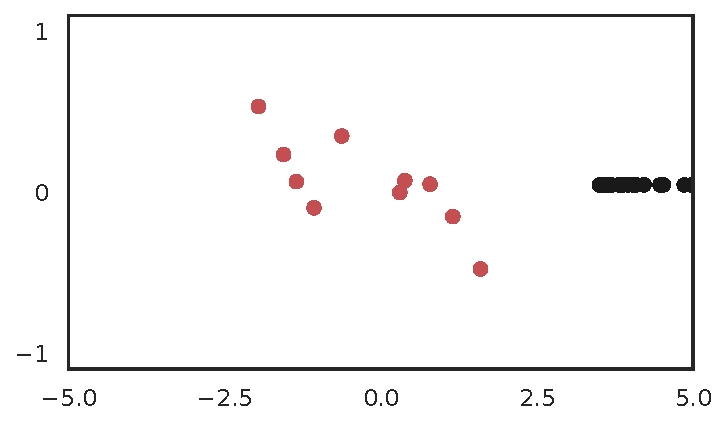
\includegraphics[width = 0.49\textwidth]{figure/direct2_pseudo.pdf}
    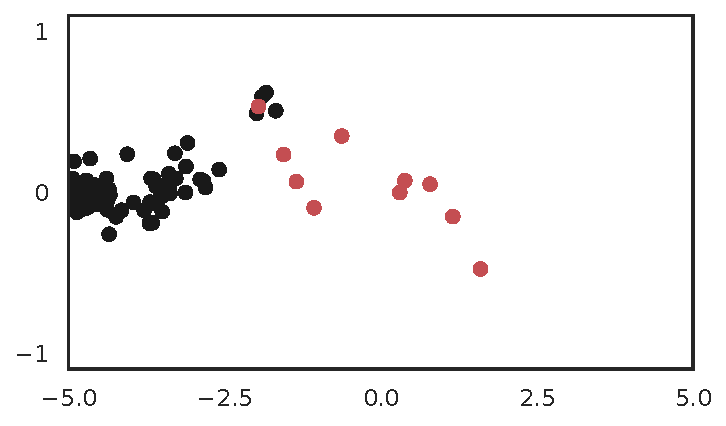
\includegraphics[width = 0.49\textwidth]{figure/direct8_pseudo.pdf}
    % \includegraphics[width = 0.32\textwidth]{figure/data plot 9.pdf}
    % \includegraphics[width = 0.32\textwidth]{figure/sample plot 9.pdf}
    % \includegraphics[width = 0.32\textwidth]{figure/posterior plot 9.pdf}
    \caption{It shows generated pseudo context dataset of direct \gls{mpanp} for 1D regression task with RBF kernel. The red dots are true context points sampled from \gls{gp} with RBF kernel, and the black dots are generated pseudo context points. (Left) Results from simultaneously generating pseudo context pair \gls{mpanp} model. (Right) Results from sequentially generating pseudo context data \gls{mpanp} model.}
    \label{fig:direct_sample}
\end{figure}
\begin{figure}[t]
    \centering
    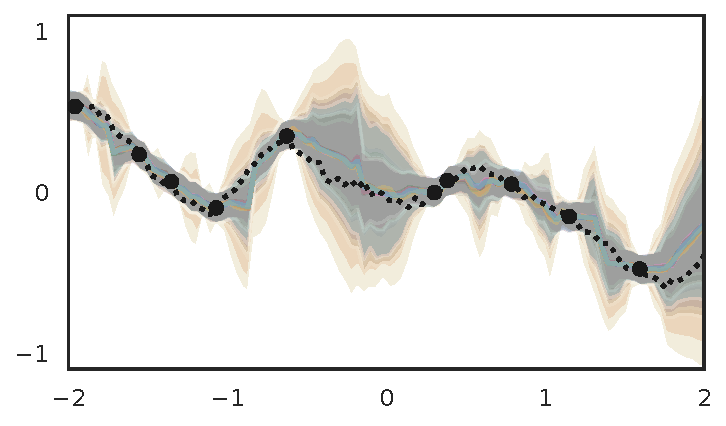
\includegraphics[width = 0.49\textwidth]{figure/direct2.pdf}
    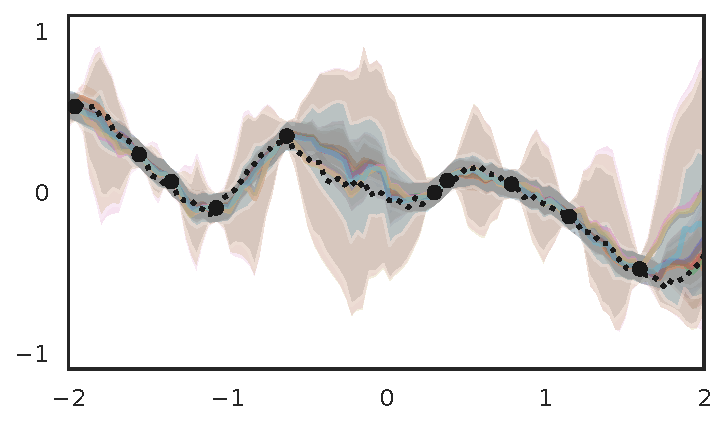
\includegraphics[width = 0.49\textwidth]{figure/direct8.pdf}
    % \includegraphics[width = 0.32\textwidth]{figure/data plot 9.pdf}
    % \includegraphics[width = 0.32\textwidth]{figure/sample plot 9.pdf}
    % \includegraphics[width = 0.32\textwidth]{figure/posterior plot 9.pdf}
    \caption{It shows posterior samples of direct \gls{mpanp} for 1D regression task with RBF kernel. The black dashed line is a function sampled from \gls{gp} with RBF kernel, and the black dots are context points. We visualized decoded mean and standard deviation with colored lines and areas. (Left) Results from simultaneously generating pseudo context pair \gls{mpanp} model. (Right) Results from sequentially generating pseudo context data \gls{mpanp} model.}
    \label{fig:direct_decode}
\end{figure}

In this section, we presents how the directly generating input model actually samples the pseudo context datasets. 

In \cref{fig:direct_sample}, we report generated pseudo context datasets and posterior samples from two different cases of directly generating input models for 1D regression task with RBF kernel. Here we can see that the generator samples pseudo context datasets far from the real context dataset. This phenomenon occurs because the generator learns to generate meaningless inputs ignored by the decoder.
In \cref{fig:direct_decode}, we report how two different directly generating \glspl{mpanp} predict posterior samples for 1D regression task with RBF kernel. 
Although directly generated pseudo context dataset are a bit far from context dataset, our model still well capture the functional uncertainty in this case.
We report the test results for 1D regression tasks on RBF for two directly generating models in \cref{table/app_gp_inf_direct}.
DSI and DSE indicate simultaneously generating models and sequentially generating models, respectively.
\cref{table/app_gp_inf_direct} shows that our directly generating models still outperform \gls{cnp} and \gls{canp} in the perspective of log-likelihood.

% In \cref{fig:direct}, we report generated pseudo context dataset from three different cases of directly generating input model.
% The first figure on the left of the \cref{fig:direct} shows the generated pseudo context samples from simultaneously generating model without the term $\calL_{\text{amort}}$ in the loss $\calL$.
% Here, we can see that the generator learns to generate meaningless inputs that are ignored by the decoder.
% The second figure on the middle of the \cref{fig:direct} shows the generated pseudo context samples from simultaneously generating model after adding the term $\calL_{\text{amort}}$ in the loss $\calL$.
% In this figure, we can see that although the model generates much more meaningful pseudo context dataset compare to the first one, still the generator fails to make sufficiently reasonable pseudo context dataset.
% The third figure on the right of the \cref{fig:direct} shows the generated pseudo context samples from sequentially generating model.
% In this figure, we can see that the model generates sufficiently meaningful pseudo context dataset compare to the others but it generates overconfidently for the unseen data points.
% Thus it fails to capture the functional uncertainty of the model which occurs the lack of the performance.
% \subsection{Long Training}

\end{document}
